\RequirePackage{fontspec}
\documentclass{ieeeaccess}
\usepackage{url}
\usepackage{cite}
\usepackage{rotating}
\usepackage[para]{threeparttablex}
\usepackage{multirow}
\usepackage{listings}
\usepackage{comment}
\usepackage{enumitem}
\usepackage{color,colortbl}
\usepackage[hidelinks]{hyperref}
\lstset{
	basicstyle=\ttfamily\footnotesize,
	escapechar=@
}
\newfontfamily\tick{DejaVu Sans}
\usepackage{amsmath,amssymb,amsfonts}
\usepackage{algorithm, algpseudocode}% <=================http://ctan.org/pkg/algorithms}\usepackage{graphicx}
\usepackage{textcomp}
\def\BibTeX{{\rm B\kern-.05em{\sc i\kern-.025em b}\kern-.08em
    T\kern-.1667em\lower.7ex\hbox{E}\kern-.125emX}}
    
\newfontfamily\mal{Manjari}[
Path=./,
UprightFont=*-Regular.ttf,
BoldFont=*-Bold.ttf
]
\newfontfamily\ipa{Gentium}[
Path=./,
UprightFont=*-R.ttf,
ItalicFont=*-I.ttf,
BoldFont=GentiumPlus-Bold.ttf
]

\definecolor{Gray}{gray}{0.9}
\bibliographystyle{unsrt}

\begin{document}
\history{Date of publication xxxx 00, 0000, date of current version xxxx 00, 0000.}
% \doi{10.1109/ACCESS.2017.DOI}
\doi{}

\title{Mlphon: A Multifunctional Grapheme-Phoneme Conversion Tool using Finite State Transducers}
\author{\uppercase{Kavya Manohar}\authorrefmark{1,3}, %\IEEEmembership{Fellow, IEEE},
\uppercase{A R Jayan\authorrefmark{2,3}, and Rajeev Rajan}.\authorrefmark{1,3}
%\IEEEmembership{Member, IEEE}
}
\address[1]{%Audio, Speech and Language Lab, Department of Electronics and Communication Engineering,
College of Engineering Trivandrum,
Kerala - 695 586 India}
\address[2]{Government Engineering College, Thrissur, Kerala, India}
\address[3]{APJ Abdul Kalam Technological University, Kerala, India }
% \tfootnote{This paragraph of the first footnote will contain support 
% information, including sponsor and financial support acknowledgment. For 
% example, ``This work was supported in part by the U.S. Department of 
% Commerce under Grant BS123456.''}

\markboth
{Kavya \headeretal: Mlphon: A Multifunctional Grapheme-Phoneme Conversion Tool}
{Kavya \headeretal: Mlphon: A Multifunctional Grapheme-Phoneme Conversion Tool}

\corresp{Corresponding author: Kavya Manohar (e-mail: sakhi.kavya@gmail.com)}


\begin{abstract}

    In this article we present the design and the development of a knowledge based computational linguistic tool, Mlphon [{\ipa em.el.foːɳ}] for Malayalam language. Mlphon computationally models linguistic rules using finite state transducers and performs multiple functions including grapheme to phoneme (g2p) and phoneme to grapheme (p2g) conversions, syllabification, phonetic feature analysis and script grammar check. This open source software tool, released under MIT license, is developed as a one-stop solution to handle different speech related text processing tasks for automatic speech recognition, text to speech synthesis and non-speech natural language processing tasks including  syllable subword based language modeling, phoneme diversity analysis and text sanity check. The tool is evaluated on a manually crafted gold standard lexicon. Mlphon performs orthographic syllabification with 99\% accuracy with a syllable error rate of 0.62\% on the gold standard lexicon. For grapheme to phoneme conversion task, overall phoneme recognition accuracy of 99\% with a phoneme error rate of 0.55\% is obtained on gold standard lexicon. Additionally an extrinsic evaluation of Mlphon is performed by employing the pronunciation lexicon created using Mlphon, in Malayalam automatic speech recognition (ASR) task. Performance analysis in terms of the computation time of lexicon creation process and the word error rate (WER) on ASR task are presented along with a comparison over other automated tools for lexicon creation. Pronunciation lexicons with more than 100k commonly used Malayalam words in phonemised and syllabified forms is created and they are published as open language resources along with this work. We also demonstrate the usage of Mlphon on different natural language processing applications - syllable subword ASR, assisted pronunciation learning, phoneme diversity analysis and text sanity check. Being a knowledge based solution with open source code, Mlphon can be adapted to other languages of similar script nature.
\end{abstract}

\begin{keywords}
	Computational Phonology, Low Resource Languages, Pronunciation Lexicon, Malayalam, Software Tool, Speech Recognition, Syllabification
\end{keywords}

% \titlepgskip=-15pt
\maketitle

\section{Introduction}

\label{intro}

Precise text processing taking care of intricate linguistic details is a pre-requisite for many downstream natural language processing (NLP) tasks. This applied research work presents the motivation and steps involved in the  development of a knowledge based computational linguistic tool, Mlphon, that can solve multiple text processing problems closely associated with speech related and some general purpose NLP tasks. Mlphon is built on finite state transducers (FSTs) to perform multiple functions including grapheme to phoneme (g2p) and phoneme to grapheme (p2g) conversions, syllabification on graphemes as well as phonemes, phonetic feature analysis, and script grammar check for Malayalam. The features of Mlphon are accessible through a programmable python API, that can be integrated with the development process of automatic speech recognition (ASR) and text to speech synthesis (TTS).

% While machine learning (ML) and deep learning (DL) based solutions gain popularity in many NLP applications, rule based ones are always preferred for core tasks where deterministic rules are available \cite{mortensen2018epitran}.  
A grapheme is the smallest functional unit of the writing system of a language and a phoneme is the smallest distinguishable sound unit of a language  \cite{Cocoulmas1999blackwellhen07,crystal2011dictionary}. The correspondence between the two, largely depends on the nature of the writing system. For grapheme-phoneme conversion tasks, most alphasyllabary languages have precise rule sets, unlike non-phonemic scripts like English \cite{mortensen2018epitran,baby2016unified}. The possible exceptions in rule sets, if any, could be handled by exception dictionaries. For languages with non-phonemic writing systems, when a sufficient amount of annotated high-quality training data is available, data driven solutions are generally preferred to extract linguistic information that is too fuzzy and difficult to be captured by a finite set of rules.
% Exceptions are easily handled by applying linguistic know-how, than in a machine learning scenario, where the system would not have access to sufficient training data especially in low resource languages . 
% For the same reason this is the approach adopted in the Epitran g2p system . 
%  A sequence of graphemes can be mapped to one or more phonemes as governed by the linguistic rules, with possible exceptions. 

% In the context of deep learning based solutions gaining popularity in various natural language processing (NLP) tasks, it is important to understand the fact that they are less viable in a low-resource setting where there is scarcity of training data. Considering the linguistic descriptions available for Malayalam, it is easier to go for a rule based approach rather than a machine learning solution. Moreover, rule based solutions can easily handle exceptions, 

%   Other than speech tasks,  Mlphon can be employed in other NLP tasks like checking for the linguistic validity of a grapheme sequence, transliterating documents in native Malayalam script to international phonetic alphabet (IPA), phonemic diversity analysis of transcribed speech corpora, syllabification for poetic metre identification etc.

Malayalam is a language spoken predominantly in the state of Kerala in southern India, with about 38 million native speakers. It belongs to the Dravidian language family, and has an alphasyllabary writing system \cite{bri1999typology}. Though Malayalam script is largely phonemic in nature, there are some unique characteristics like: (i) consonants with and without inherent vowel, (ii) consonant clusters with pronunciation different from the consonants present in them, (iii) special symbol \textit{virama}, that contextually chooses its function depending on its position in a word and (iv) graphemes being overloaded with non-native sounds in loan words. %\footnote{See Section \ref{arch} for details}. 

Rule based mappings between graphemes and phonemes are basically context-sensitive rewrite rules. Each rule specifies how a set of symbols get mapped to another set. FSTs provide efficient methods for performing the composition of such rule sets to single mega rule as described in \cite{kaplan1994regular} and \cite{karttunen1992two}. This has made FST popular in many fundamental NLP applications \cite{oflazer2006architecture,anberbir2011grapheme, mortensen2018epitran,thottingal-2019-finite,kayabacs2019trmor}. The rule set of Mlphon is written in Stuttgart finite state toolkit (SFST) formalism and compiled to FSTs \cite{schmid2005programming}. 
% The system architecture of Mlphon and its implementation as composition of FSTs is presented in this article.


The rest of this article is organized as follows. Section \ref{motivation} provides the motivation behind the proposed tool and section \ref{literature} explains how it relates to similar tools reported in literature. Section \ref{graphemes} describes the nature of grapheme and phoneme inventories of Malayalam and section \ref{syllablestructure} explains the computational rules of Malayalam script syllabification. Section \ref{arch} describes the design and development of Mlphon and explains how the linguistic rules are incorporated in Mlphon architecture.  Section \ref{goldlexicon} presents the evaluation of Mlphon against a gold standard reference. Performance analysis and comparison with other lexicon creation tools on ASR task is presented in section \ref{asr}. The usage of Mlphon to create the largest openly available pronunciation lexicon for Malayalam is described in section \ref{pronunciationdictionary}.
% Section \ref{asr} explains the use of the pronunciation lexicon to create a large vocabulary Malayalam ASR and its performance comparison with other automated tools available for lexicon creation.
Section \ref{applications} describes the applications of Mlphon in text sanity check, assisted pronunciation learning, phoneme diversity analysis and syllable subword based ASR. Section \ref{conclusion} concludes the article with a summary of the work.

\section{MOTIVATION}
\label{motivation}

Solutions for automatic g2p conversion in one language may not be the optimal solution applicable for a different language. There are problems with different levels of difficulty that should be solved for each language or language family separately \cite{mdpi2022ruleg2p}. Malayalam is a morphologically complex low resource language with very little transcribed audio datasets and no openly available pronunciation lexicons. Morphologically complex languages with very large number of rare words are challenging for machine translation and ASR tasks due to huge out of vocabulary (OOV) rate. Malayalam language is known to demonstrate a high level of morphological complexity than many other Indian and European languages in terms of type-token ratio and type-token growth rate \cite{manohar2020quantitative, bharadwaja2007statistical}. 
% It is the proportion of words that are not present in the vocabulary and thus cannot be recognized or translated correctly.
For languages with very little transcribed audio datasets available for speech related tasks, a precise grapheme to phoneme conversion can ensure better acoustic modeling, even in end-to-end \cite{baevski2021unsupervised} ASR systems. 


Segmenting words to syllables has got its applications in machine translation systems and speech to text systems especially in the context of morphologically complex languages where subword level units improve system performance \cite{kunchukuttan2016, SMIT2021101158}. In many languages, g2p correspondence depends on the relative position of grapheme within a word and a syllable, which makes syllable boundary identification further more important for phoneme level analysis. In the era of large language models being built on web crawled text corpora \cite{kunchukuttan2020ai4bharat}, it is necessary to ensure the sanity of text. Checking for the linguistic validity of character sequences can guarantee this to a large extent.

Availability of a ready to use pronunciation lexicon is an essential linguistic resource for ASR (DNN/HMM pipeline model) and TTS tasks. There are machine readable pronunciation dictionaries available for various world languages. CMUDict is an open source machine readable pronunciation lexicon for North American English that contains over 134k words and their pronunciations \cite{lenzo2007cmu}. Similar efforts for creating pronunciation lexicons for different world languages are reported in literature, namely; Globalphone, providing pronunciation lexicon of 20 world languages  \cite{schultz-schlippe-2014-globalphone}, the LC-STAR Phonetic Lexica of 13 different languages  \cite{castell2004lc}, Arabic speech recognition pronunciation lexicon with two million pronunciation entries for 526k Modern Standard Arabic words \cite{ali2017}, ASR oriented Indian English pronunciation lexicon  \cite{huang-etal-2020-construction}, manually curated Bangla phonetic lexicon of 65k lexical entries prepared for TTS  \cite{ttsbangla}, to mention a few.

However openly available large vocabulary pronunciation lexicon has not been reported for Malayalam, till date. The reported works on Malayalam pronunciation lexicons has mostly been done manually or semi-automatically with a small or medium vocabulary for ASR tasks \cite{cinikurian,deekshitha}. Agricultural speech and text corpora for Malayalam with 4k manually transcribed phonetic lexicon entries has been  reported by Lekshmi et al. \cite{k-r-etal-2020-malayalam}. Considering the agglutinative nature of Malayalam language and its practically infinite vocabulary, a manually curated, small sized pronunciation lexicon would be inadequate for general domain speech tasks \cite{manohar2020quantitative}.  Also there could be need for expanding the vocabulary of lexicon as new words get added to the language in the form of proper nouns and loan words. These lexicons can serve as high quality annotated data sets for bootstrapping data driven g2p training.


% \subsection*{Motivation}

The need to perform precise grapheme to phoneme conversion on demand, to perform syllabification on graphemes as well as phonemes, and to create a programmable API for integrating these functionalities on downstream NLP tasks prompted us to develop the multifunctional tool Mlphon. Our decision to use a knowledge-based approach was driven by the availability of adequate linguistic descriptions. Even though there has been many previous attempts to address one or more of these problems, Mlphon offers certain unique features compared to these prior works which makes it a well suited tool for ASR related tasks in Malayalam. 

\section{Related Works}
\label{literature}

Data driven and knowledge based  approaches are the two main g2p strategies. While languages with sufficient amounts of annotated data for training primarily rely on data driven techniques, languages with well documented pronunciation rule sets use knowledge based solutions. In the former, the g2p rules are learned directly from data, whereas in the latter, rules are constructed using linguistic expertise.

Data driven approaches perform g2p mapping by dictionary lookups \cite{black1998issues}, decision trees \cite{black1998issues}, conditional random fields \cite{fosler2013conditional}, pronunciation by analogy \cite{yvon1996grapheme} or joint sequence alignments \cite{bisani2008joint}. Recently deep learning architectures for g2p developed based on recurrent neural networks \cite{yao2015sequence}, convolutional neural networks \cite{yolchuyeva2019grapheme}  and transformers \cite{sevinj2019transformer}. Zero shot g2p learning techniques without explicit training data have been proposed, but they are based on the assumption that similar language families use the same orthography, which is not always true \cite{li-etal-2022-zero}. Phonetisaurus \cite{novak_minematsu_hirose_2016} is a data driven tool that learns the  mapping rules statistically (joint sequence models) from a training dataset and builds weighted FSTs for g2p conversion. Malayalam does not have a good quality annotated data set for g2p training and a Phonetisaurus model for Malayalam has not yet been reported. 

For languages with regular grapheme to phoneme conversion patterns, knowledge-based g2p has been reported to produce good results \cite{li-etal-2022-zero, sar2019applying}. A set of sequential rewrite rules can be used to achieve this. Agglutinative languages like Turkish \cite{oflazer2006architecture} and Amharic \cite{anberbir2011grapheme} have reported works on language specific knowledge based g2p conversion using FST technology. Epitran \cite{mortensen2018epitran}, an open source tool using rule based FSTs for g2p conversion of more than 61 world languages recently added Malayalam support, with preliminary mapping between graphemes and phonemes. Hybrid approaches that applies linguistic rules on statistical g2p mappings have been reported for Khmer language \cite{sar2019applying}. 



% Implementation of rule-based approaches require thorough linguistic know-how.
\subsection{Requirement Analysis: A Comparison with Related Tools in Malayalam}


\begin{table}[!h]
	\begin{center}
		\begin{minipage}{280pt}
			\caption{Comparing the functionalities and features of grapheme - phoneme \\conversion tools in Malayalam}
			\label{tools}
			\begin{tabular}{@{}lccccccccc@{}}
\\ \hline \hline
				Tools &  \rotatebox{90}{Script Grammar Check}&\rotatebox{90}{Orthographic Syllabification}& \rotatebox{90}{Grapheme to Phoneme} & \rotatebox{90}{Phoneme Delimiter} & \rotatebox{90}{Phoneme Syllabification} & \rotatebox{90}{Phoneme to Grapheme}  & \rotatebox{90}{Phonetic Feature Analysis}&\rotatebox{90}{Open source}&\rotatebox{90}{Programmable API} \\
				\hline
				Unified Parser  \cite{baby2016unified}                 &      &           & {\tick ✓} &{\tick ✓}&{\tick ✓}&           &       &{\tick ✓} &  \\
				Espeak  \cite{duddington2012espeak}                         &      &           & {\tick ✓} &{\tick ✓}&{\tick ✓}&           &       &{\tick ✓}& {\tick ✓}\\
				Festvox \cite{parlikar2016festvox}                &      &           & {\tick ✓} &{\tick ✓}&{\tick ✓}&           &       &{\tick ✓}\\

				Aksharamukha\cite{aksharamukha}                     &      &           &{\tick ✓} &          &         &{\tick ✓}  &       &{\tick ✓}& {\tick ✓}\\
				Indic NLP \cite{kunchukuttan2020indicnlp}                     &      &{\tick ✓}  & {\tick ✓} &         &         &           &       &{\tick ✓}& {\tick ✓}\\
				% Epritan \cite{mortensen2018epitran}                     &      &{\tick ✓}  & {\tick ✓} &         &         &           &       &{\tick ✓}\\
				Code-switched \cite{manghat2020malayalam}  &      &           &{\tick ✓} & {\tick ✓}&         &           &       & \\
				LTS \cite{aswathy2014improving}  &      &           &{\tick ✓} & {\tick ✓}&         &           &       &&\\

				Encoder-Decoder \cite{Priyamvada_2021} &   & & {\tick ✓} & {\tick ✓} &   &  & &\\
				\hline
				\textbf{Mlphon}                 & {\tick ✓} &{\tick ✓}& {\tick ✓} &{\tick ✓}&{\tick ✓}&{\tick ✓}& {\tick ✓}&{\tick ✓}& {\tick ✓}\\

				\hline
			\end{tabular}
		\end{minipage}
	\end{center}
\end{table}
This section focuses on related tools that works for Malayalam. Being a language with regular orthography, most of the  g2p conversion tools in Malayalam follow  knowledge based approaches \cite{duddington2012espeak,baby2016unified,parlikar2016festvox,aksharamukha,kunchukuttan2020indicnlp,manghat2020malayalam,aswathy2014improving} rather than data driven methods. 
% This is primarily due to the availability of deterministic rules sets and secondarily due to unavailability of annotated data for training. 
The only data driven method is based on encoder-decoder architecture \cite{Priyamvada_2021} and uses data prepared using an existing knowledge based solution. Table \ref{tools} compares the functionalities of different grapheme-phoneme conversion tools available for Malayalam. Here, we examine each of their features and drawbacks in detail:

\begin{itemize}
    \item Unified parser \cite{baby2016unified} is a multi-lingual open source tool for parsing Indian languages and converting it to a common label set of phonemes in syllabified form. In its language-specific logic, it doesn't take into account any of the Malayalam pronunciation modification rules other than the addition of inherent vowels. This tool does not syllabify graphemes.
    \item Espeak \cite{duddington2012espeak} is an open source speech synthesis system that has a g2p module and it supports Malayalam. Even though phoneme syllabification is supported by Espeak, it does not syllabify graphemes.
    \item Festvox Indic frontend perform g2p, for TTS systems. It uses X-SAMPA phone set \cite{parlikar2016festvox}. On analysing the transcription it provides,  many contextual rules are observed to be missing for Malayalam and it does not support syllabification of graphemes. 
    % This tool also supports many language specific rules, but not all. 
    \item Aksharamukha \cite{aksharamukha} script converter is an open source tool that supports g2p for many languages. However language specific contextual logic is lacking for Malayalam. It can not be used to create a pronunciation lexicon, as it does not provide delimiters between phonemes. It syllabifies neither graphemes nor phonemes.
    % \footnote{Espeak TTS: \url{http://espeak.sourceforge.net/}}.
    \item The Indic NLP library \cite{kunchukuttan2020indicnlp}, supports syllabification of graphemes and performs g2p. This tool lacks delimiters between phonemes, so it cannot be used to create a pronunciation lexicon.
    \item
     FST based g2p mapping for code switched Malayalam-English text has been reported in \cite{manghat2020malayalam}, where English words are phoneme mapped using CMUDict\footnote{CMUDict- The CMU Pronouncing Dictionary: \url{http://www.speech.cs.cmu.edu/cgi-bin/cmudict}} and contextual rule based FST was used for Malayalam. This tool is not open source and hence not freely available for further use, research or analysis.
    \item
    Using basic letter to sound (LTS) rules, an automatic pronunciation lexicon creation work was proposed in \cite{aswathy2014improving}. It uses a naive Bayes classifier to identify native and English language words and use different set of LTS to perform the g2p mapping. This tool is not openly available for further research and analysis.
     \item The only deep learning based data driven approach for Malayalam g2p conversion uses Unified Parser for creating the data set for training and testing the model \cite{Priyamvada_2021}. It has the same features and shortcomings as the Unified Parser tool.
\end{itemize}



%  However these tools for Malayalam are restrictively licensed and not openly available for testing.
Based on our detailed analysis of the available tools cited above, it was found that none of these tools have full coverage of pronounceable characters defined in Malayalam Unicode.  None of these tools could handle the overloading of the letters {\mal ഫ }(labiodental fricative and and also as labial aspirated plosive) {\mal ന }(dental nasal and also as alveolar nasal) and their disambiguation. Each of these tools follow different choice of phonetic alphabets and mapping criteria, making them incompatible for a meaningful comparison.

% An DNN/HMM hybrid ASR system requires the graphemes to be represented as a sequence of phonemes in the pronunciation lexicon with delimiters in between. The Unified Parser, Indic Front end and Espeak provides lexicon in this format. Only Espeak implements the most common digression in Malayalam g2p mapping, the contextual substitutions needed in alveolar nasal/plosive conjuncts.

    %  \item 

% Even though Unified Parser and Indic Front end provides syllabification (delimiter between syllables in the phonemized text), they do not syllabify the native script. So a syllable level mapping between graphemes and phonemes is can not be provided by these tools. Aksharamukha provides bidirectional conversion between graphemes and phonemes, but syllabify neither native script nor phonemes. Indic NLP library is an open source python library that provides syllabification of native script, but does not provide phonemes with delimiters in between. E

 \subsection{Key Contributions}
 
% Mlphon is developed as an open source python library that performs g2p and p2g mapping, syllabification of graphemes as well as phonemes and supports all pronounceable Malayalam Unicode characters. It additionally provides phonetic feature information. The utilities provided by Mlphon are made accessible through programmable APIs, which can be easily integrated into various applications like Kaldi ASR Training.  The key contributions of this work are the development a knowledge based computational linguistic tool for precise syllabification and bidirectional grapheme-phoneme conversion. 

% The utility functions provided by these tools are listed in Table \ref{tools}. To the best of our knowledge, Mlphon presented in this article, is the only  single open source tool that performs all of script validity checks, bidirectional grapheme-phoneme conversions, orthographic syllabification and phonetic feature tagging for Malayalam script.


 
The key contributions of this applied research work are:
 
 \begin{enumerate}
% 	\item A linguistic exploration of the grapheme and phoneme inventories of Malayalam language and the relation between the two.
% 	\item A linguistic description of the orthographic syllabification rules for Malayalam.
	\item The design and development of a knowledge based computational linguistic tool, Mlphon. It is the only tool with a programmable interface that can do every one of the following:
	      \begin{itemize}
		      \item Syllabification on graphemes as well as phonemes.
		      \item Phonetic feature analysis.
		      \item g2p and p2g conversions.
      \end{itemize}

	% \item The creation of a hand-curated, gold-standard phonemic lexicon for Malayalam with inputs from linguistic experts.
    \item Evaluation of Mlphon in comparison to a gold standard lexicon.
    \item Comparison of Mlphon with other openly available tools for lexicon creation and their application on ASR task.
	\item The publication of a large vocabulary pronunciation lexicon for Malayalam. 
% 	Apart from 100k common words, it includes curated collection of verbs, nouns and commonly used non-native words in Malayalam script. The pronunciations are available in phonemized and syllabified form. This ready to use, large vocabulary, open lexical resource is the first of its kind in Malayalam language.
	\item A description of the usage of Mlphon on various NLP applications:
	\begin{itemize}
			 \item Syllable level language modeling for open vocabulary ASR.
    	      \item Web based tool for assisted pronunciation learning.
		      \item Script sanity check and correction.
		      %\item Large vocabulary ASR

	      \end{itemize}
	\item Openly licensed resources and source codes (Appendix \ref{resources}).
	      %    The performance in terms of word error rate (WER) is evaluated and compared with other automated tools for lexicon creation.

\end{enumerate}




\section{Grapheme Inventory of Malayalam}
\label{graphemes}

Malayalam belongs to the family of Brahmic writing systems that is alphasyllabary in nature  \cite{bri1999typology}. In this writing system, consonant - vowel sequences are written as a unit; each unit is based on a consonant character, and the vowel notation is secondary. The basic components in Malayalam orthography belong to three classes of characters: namely vowels, consonants and signs. Additionally there are complex graphemes derived from these basic characters.
%In the digital representation of Malayalam text, every valid Malayalam character has a unique value universally defined by Unicode standard. In the current standard 14.0, there are 118 Malayalam characters each with a unique code point\footnote{See page 518 of the Unicode chart: \url{http://www.unicode.org/versions/Unicode14.0.0/ch12.pdf}}.

\begin{table*}[h]
	\begin{center}
		\begin{minipage}{\textwidth}
			\caption{Short and long vowels in Malayalam and their IPA representations}\label{vowelgrapheme}%
			\begin{tabular}{@{}l|llllllllllllllll@{}}
				\hline \hline
		Vowels   & {\mal അ} {\ipa a}& {\mal ആ} {\ipa aː}   & {\mal ഇ} \ipa{i} & {\mal ഈ} \ipa{iː }  & {\mal ഉ} {\ipa u} & {\mal ഊ} {\ipa uː}  & {\mal ഋ} {\ipa rɨ} & {\mal ൠ} {\ipa rɨː}& {\mal ഌ} {\ipa lɨ} & {\mal ൡ} {\ipa lɨː}& {\mal എ} {\ipa e} & {\mal ഏ} {\ipa eː }& {\mal ഐ} {\ipa ai}      & {\mal ഒ} {\ipa o} & {\mal ഓ} {\ipa oː} & {\mal ഔ} {\ipa au}\\ \hline
             
				Vowel Signs  & {\mal }           & {\mal ാ}           & {\mal ി}         & {\mal ീ}           & {\mal ു}           & {\mal ൂ} & {\mal ൃ}            & {\mal ൄ}             & {\mal ൢ}            & {\mal ൣ}            & {\mal െ}          & {\mal േ}     & {\mal ൈ}                & {\mal ൊ}          & {\mal ോ}         & {\mal ൗ ൌ}     \\
				\hline
			\end{tabular}
		\end{minipage}
	\end{center}
\end{table*}

% \subsection{Basic Components in Malayalam Orthography}
% \label{basiccharacters}

%  A discussion on the peculiarities of each of these classes and the correspondence of these graphemes with phonemes are discussed in the sections that follow.

% (iv) Archaic characters and (v) Numbers. \footnote{Script notes on Malayalam by Richard Ishida:\url{https://r12a.github.io/scripts/malayalam/}},


\subsection{Vowels}

There are 16 vowels in Malayalam. It includes 5 short vowels, 5 long vowels, 2 diphthongs and 4 vocalics  \cite{asher1997}. Independent vowels occur only at word beginnings. Vowels that follow consonants in word medial or end positions are indicated by dependent vowel signs. Consonants generally have the vowel {\ipa /a/} inherent in them, eliminating the need for specialized vowel sign for {\mal അ} {\ipa /a/}. See Table \ref{vowelgrapheme} for the list of all vowels in Malayalam and their IPA representations.


% \begin{table}[h]
% 	\begin{center}
% 		\begin{minipage}{140pt}
% 			\caption{Diphthongs in Malayalam and their IPA representations}\label{diphthonggrapheme}%
% 			\begin{tabular}{@{}lll@{}}
% 				\hline
% 				Vowels      & {\mal ഐ} {\ipa ai} & {\mal ഔ} {\ipa au} \\

% 				Vowel signs & {\mal ൈ}           & {\mal ൗ, ൌ}        \\
% 				\hline
% 			\end{tabular}
% 		\end{minipage}
% 	\end{center}
% \end{table}

% \begin{table}[h]
% 	\begin{center}
% 		\begin{minipage}{170pt}
% 			\caption{Vocalics in Malayalam and their IPA representations}\label{vocalicgrapheme}%
% 			\begin{tabular}{@{}lllll@{}}
% 				\hline
% 				Vowels      & {\mal ഋ} {\ipa rɨ} & {\mal ൠ} {\ipa rɨ}ː & {\mal ഌ} {\ipa lɨ} & {\mal ൡ} {\ipa lɨː} \\

% 				Vowel signs & {\mal ൃ}            & {\mal ൄ}             & {\mal ൢ}            & {\mal ൣ}             \\
% 				\hline
% 			\end{tabular}
% 		\end{minipage}
% 	\end{center}
% \end{table}

\subsection{Consonants}

There are 38 regular consonant graphemes in Malayalam \cite{asher1997}. This includes 21 plosives classified by their aspirational and voicing characteristics, 6 nasals, 4 fricatives, 3 approximants, 2 laterals and 1 each tap and trill. The place of articulation are indicated in the rows and manner of articulation in the columns of the Table \ref{consonantgrapheme}. Apart from the regular consonants, there are dead consonants (referred as \textit{chillus}) in Malayalam, which do not have the inherent vowel associated with them. The \textit{chillus} of Malayalam are listed in Table \ref{chillus}. 
% Linguistically chillus are not allowed to have any dependent vowel signs or \textit{virama} to follow them, except for an alternate representation for the consonant cluster {\mal ന്റ} {\ipa /nṯa/}.

\begin{table*}
	\begin{center}
  \begin{threeparttable}
  \caption{Consonants in Malayalam and their IPA representations}\label{consonantgrapheme}
			% \setcounter{mpfootnote}{\value{footnote}}
			% Redefine the command that produces the footnote number
			% \renewcommand{\thempfootnote}{\arabic{mpfootnote}}
			\begin{tabular*}{\textwidth}{@{\extracolsep{\fill}}llccccccccccc@{\extracolsep{\fill}}}
				\hline% \hline
				\textbf{Place of }& \multicolumn{9}{@{}c@{}}{\textbf{Manner of Articulation}}\\
				\textbf{Articulation} & Plosive\tnote{a} & Plosive\tnote{b} & Plosive\tnote{c} & Plosive\tnote{d}                        & Nasal        & Trill        & Tap          & Fricative   & Approximant      & Lateral                                               \\

				\hline
				Velar                        & {\mal ക} {\ipa ka}                                         & {\mal ഖ} {\ipa kʰa}& {\mal ഗ}  {\ipa ɡa} & {\mal ഘ} {\ipa ɡʰa} & {\mal ങ} {\ipa ŋa} &              &             &             &                           \\
				%\hline
				% IPA & {ka } & {kʰa}  & {ɡa} & {ɡʰa} & {ŋa} & \\
				Palatal                      & {\mal ച} {\ipa ca}                                         & {\mal ഛ} {\ipa cʰa} & {\mal ജ} {\ipa ɟa}  & {\mal ഝ} {\ipa ɟʰa} & {\mal ഞ} {\ipa ɲa} &              &             & {\mal ശ} ɕa & {\mal യ} ja               \\
				% \hline
				% IPA & {ca} & {cʰa}  & {ɟa} & {ɟʰa} & {ɲa} & \\

				Retroflex                    & {\mal ട} {\ipa ʈa}                                         & {\mal ഠ} {\ipa ʈʰa} & {\mal ഡ} {\ipa ɖa}  & {\mal ഢ} {\ipa ɖʰa} & {\mal ണ} {\ipa ɳa} &              &             & {\mal ഷ} ʂa & {\mal ഴ} ɻa & {\mal ള} {\ipa ɭa} \\


				Alveolar                     & {\mal ഺ} {\ipa ṯa}                                         &              & {\mal }      & {\mal}       & {\mal ഩ} {\ipa na} & {\mal  റ} {\ipa ra} & {\mal ര} {\ipa ɾa} & {\mal സ} {\ipa sa} &             & {\mal ല} {\ipa la} \\
				%  \hline
				%  IPA & {ʈa } & {ʈʰa}  & {ɖa} & {ɖʰa}  & {ɳa} & \\

				%  \hline
				%  \hline
				Dental                       & {\mal ത} {\ipa t̪a}                                         & {\mal ഥ} {\ipa t̪ʰa} & {\mal ദ} {\ipa d̪a}  & {\mal ധ} {\ipa d̪ʰa} & {\mal ന} {\ipa n̪a} &              &             &             &                           \\
				%  \hline
				% IPA & {t̪a} & {t̪ʰa}  & {d̪a} & {d̪ʰa} & {n̪a} & \\

				% \hline
				% \hline
				Labial                       & {\mal പ} {\ipa pa}                                         & {\mal ഫ} {\ipa pʰa} & {\mal ബ} {\ipa ba}  & {\mal ഭ} {\ipa bʰa} & {\mal മ} {\ipa ma} &              &             &             &                           \\
				% \hline
				% IPA & {pa} & {pʰa}  & {ba} & {bʰa} & {ma} & \\

				Labiodental                  &                                                     &              &              &              &             &              &             &             & {\mal വ} {\ipa ʋa}               \\
				Glottal                      &                                                     &              &              &              &             &              &             & {\mal ഹ} {\ipa ha} &                           \\
				\hline
			\end{tabular*}
       \begin{tablenotes}
       \item [a] Unaspirated and Unvoiced        \item [b] Aspirated and Unvoiced \item [a] Unapirated and Voiced \item [a] Aspirated and Voiced
       \end{tablenotes}

  \end{threeparttable}	
  \end{center}
\end{table*}


\begin{table}
	\begin{center}
		\begin{minipage}{\linewidth}
			\caption{\textit{Chillus} in Malayalam and their IPA representations. Top row lists the \textit{chillus} and the corresponding bottom row shows the base consonants from which \textit{chillus} were derived.}\label{chillus}%
			\begin{tabular}{@{}ccccccccc@{}}
				\hline\\
				  {\mal ൿ} {\ipa k} &{\mal ൺ} {\ipa ɳ}&{\mal ൻ} {\ipa n}&{\mal ൽ} {\ipa l}& {\mal ൔ} {\ipa m}&{\mal ൕ} {\ipa j}& {\mal ൾ} {\ipa ɭ}& {\mal ൖ} {\ipa ɻ}& {\mal ർ} {\ipa r} \\
				\hline                                                                                                                                                                            
    {\mal ക} {\ipa ka}& {\mal ണ} {\ipa ɳa}&{\mal ന} {\ipa na}& {\mal ല} {\ipa la}&{\mal മ} {\ipa ma}&{\mal യ} {\ipa ja}&{\mal ള} {\ipa ɭa}&{\mal ഴ} {\ipa ɻa}&{\mal ര} {\ipa ra}\\
				\hline
			\end{tabular}
		\end{minipage}
	\end{center}
\end{table}

\subsection{Signs}

The special signs  \textit{virama} ({\mal ്}),  \textit{dot reph }({\mal ൎ}),  \textit{anuswara} ({\mal ം}) and \textit{visarga} ({\mal ഃ}) have their properties as tabulated in Table \ref{signs}. \textit{Virama} removes the inherent vowel from the consonant preceding it. The virama that occurs at word ends, apart from removing the inherent vowel, adds the mid-central vowel schwa {\ipa /ə/} to native Malayalam words. \textit{Dot reph} is an alternate sign representation for the consonant clusters that begin with {\ipa /r/} or {\ipa /ɾ/}. \textit{Anuswara}  is a sign common in Malayalam. Its phonemic representation is {\ipa /m/} and always mark syllable endings. \textit{Visarga} sign is popular in Sanskrit derived words and they introduce slight pronunciation changes similar to aspirated glottal stop.

\begin{table}[]
    \caption{Signs in Malayalam}
    \label{signs}
\begin{tabular}{l|l}
\hline \hline
\textbf{Sign} & \textbf{Properties} \\ \hline
\textit{Anuswara} ({\mal ം}) &  Represents /m/ at syllable ends. \\
 \textit{Dot reph }({\mal ൎ}) & Represents {\ipa /r/} or {\ipa /ɾ/}.  \\
\textit{Visarga} ({\mal ഃ}) & Introduces aspirated glottal stop. \\
\textit{Virama} ({\mal ്}) & Kills Inherent vowel. \\
 & Inserts schwa at  word ends. \\ 

\hline \hline
\end{tabular}


\end{table}

%Consonant clusters  are formed when two or more consonants are joined by virama sign in between. For example, the sequence {\mal ക} /ka/, {\mal ്} (virama), {\mal ഷ} /ʂa/ results in the consonant cluster {\mal ക്ഷ} /kʂa/. More details on consonant clusters is available in section \ref{complexgraphemes}


% The exact phonemic representation of this sign depends on the consonants following them. It always occur at the beginning of an orthographic syllable.

%  is a sign common in Malayalam. Its phonemic representation is {\ipa /m/} and always mark syllable endings.


\subsection{Complex Graphemes in Malayalam}
\label{complexgraphemes}

Apart from the basic characters, Malayalam script has hundreds of complex graphemes representing consonant clusters. A consonant cluster is a sequence of consonants with no intervening vowels. The removal of inherent vowel from the conjoining consonants happens on the addition of a \textit{virama} sign. A consonant cluster, often forms a complex grapheme with one or more of stacking, changing and merging the shapes of the constituent characters. Hundreds of possible complex graphemes in Malayalam are not individually encoded in Unicode, instead they are constituted from basic characters. Table \ref{complexgraphemetable} lists certain examples of consonant clusters in Malayalam and their constituents.


\begin{table}[h]
	\begin{center}
		\begin{minipage}{210pt}
			\caption{Examples of consonant clusters in Malayalam and their constituents}\label{consonantclusters}%
            \label{complexgraphemetable}
			\begin{tabular}{@{}c|ccccc@{}}
				\hline \hline
				\textbf{Consonant cluster}      & \multicolumn{5}{c}{\textbf{Constituent character sequence}}                                                               \\
				\hline
				{\mal ക്ക} {\ipa kka}   & {\mal ക} {\ipa ka}                                 & {\mal ്} & {\mal ക} {\ipa ka}                                \\
				{\mal ങ്ക} {\ipa ŋka}   & {\mal ങ} {\ipa ŋa}                                 & {\mal ്} & {\mal ക} {\ipa ka}                                \\
				{\mal ക്ല} {\ipa kɭa}   & {\mal ക} {\ipa ka}                                 & {\mal ്} & {\mal ല} {\ipa la}                                \\
				{\mal ഘ്ന} {\ipa ɡʱna}  & {\mal ഘ} {\ipa ɡʱa}                                & {\mal ്} & {\mal ന} {\ipa n̪a}                                \\
				{\mal സ്ത} {\ipa st̪a}   & {\mal സ} {\ipa sa}                                 & {\mal ്} & {\mal ത} {\ipa t̪a}                                \\
				{\mal ഗ്ര} {\ipa gɾa}   & {\mal ഗ} {\ipa ga }                                & {\mal ്} & {\mal ര} {\ipa ɾa}                                \\
				{\mal ഗ്യ} {\ipa gja}   & {\mal ഗ} {\ipa ga}                                 & {\mal ്} & {\mal യ} {\ipa ja}                                \\
				{\mal ന്ത്ര} {\ipa n̪t̪ra} & {\mal ന} {\ipa n̪a}                                 & {\mal ്} & {\mal ത} {\ipa t̪a} & {\mal ്} & {\mal ര} {\ipa ɾa} \\
\hline
				\hline
			\end{tabular}
		\end{minipage}
	\end{center}
\end{table}

% A consonant cluster has a structure of the following form:

% \begin{verbatim}
% consonant cluster = consonant (+ \textit{virama} + consonant)*
% \end{verbatim}
% \noindent{\ipawhere * represents one or more number of repetitions}

% The simplest consonant cluster has two consonants conjoined by a virama in between. The inherent vowel sound of consonants before virama gets removed in the process. 
%There is no rule which limits the number of consonants involved in the formation of a conjunct. 
% Certain consonant clusters that end in {\mal യ} {\ipa /ja/}, {\mal ര} {\ipa /ɾa/}, {\mal ല} {\ipa /la/}, {\mal വ} {\ipa /ʋa/} form special signed shapes. 




\begin{comment}

\section{Phoneme Inventory of Malayalam}
\label{phonemes}


The regular vowel phonemes in Malayalam are listed in Table \ref{vowelphoneme}, classified with their vowel height, length and backness. The graphemic origin of these vowel phonemes can be from independent vowels or dependent vowel signs. The mid-central vowel, schwa ({\ipa /ə/}) does not have a specific vowel grapheme. Its occurrence is limited to words that end in \textit{virama}. Discussion on schwa addition at word ends is in Section \ref{virama}. Additionally there are two diphthongs ({\ipa /ai/}, {\ipa /au/}) and four vocalics ({\ipa /rɨ/}, {\ipa /rɨː/}, {\ipa /lɨ/}, {\ipa /lɨː/}) in Malayalam which belongs to the category of vowels. Vocalics are letters derived from Sanskrit that generally behave like vowels\footnote{Script notes on Malayalam by Richard Ishida: \url{https://r12a.github.io/scripts/malayalam/}} \cite{asher1997}.

\begin{table}[h]
	\begin{center}
		\begin{minipage}{210pt}
			\caption{Vowel phonemes of Malayalam}\label{vowelphoneme}%
			\begin{tabular}{@{}llcccccc@{}}
				\hline
				                                                       &           & \multicolumn{5}{c}{\textbf{Vowel Backness}}                                                               \\

				                                                       &           & \multicolumn{2}{c}{Front}                   & Central   & \multicolumn{2}{c}{Back}                        \\
				%
				                                                       &           & Short                                       & Long      & Short                    & Short    & Long      \\
				\hline
				\multirow{4}{*}{\rotatebox{90}{\textbf{Vowel Height}}} & Close     & {\ipa i }                                   & {\ipa iː} &                          & {\ipa u} & {\ipa uː} \\

				                                                       & Close-mid & {\ipa e}                                    & {\ipa eː} &                          & {\ipa o} & {\ipa oː} \\
				                                                       & Mid       &                                             &           & {\ipa ə}                 &                      \\

				                                                       & Open      & {\ipa a}                                    & {\ipa aː} &                          &          &           \\
				\hline
			\end{tabular}
		\end{minipage}
	\end{center}
\end{table}

There are 39 consonant phonemes in Malayalam. Their classification based on the manner and place of articulation is listed in Table \ref{consonantphonemes}.  The plosive phonemes in Malayalam have the features of aspiration and voicing. Native Malayalam words do not have the phoneme labiodental fricative, {\ipa /fa/}. But a lot of foreign language words are written by overloading the labial aspirated plosive grapheme {\mal ഫ} {\ipa /pʰa/} with the {\ipa /fa/} sound.  This makes the consonant phoneme inventory larger than the consonant grapheme inventory by one. Disambiguating the pronunciations of {\mal ഫ}, primarily involves identifying if it is a foreign language word from the grapheme context.
% Implementation of this rule is explained in section \ref{labiodentalfricative}.
% The commonly used phoneme /f/, the labiodental fricative, is represented by overloading the grapheme {\mal ഫ} /pʰa/.
The correspondence of the phonemes with the graphemes in Malayalam script and the rules of exceptions are discussed in Section \ref{g2p}


\begin{table}[h]
	\begin{center}
		\begin{minipage}{\textwidth}
			\caption{Consonant Phonemes of Malayalam}\label{consonantphonemes}%
			\setcounter{mpfootnote}{\value{footnote}}
			% Redefine the command that produces the footnote number
			\renewcommand{\thempfootnote}{\arabic{mpfootnote}}
			\begin{tabular}{@{}lllccccccccccc@{}}
				\hline
				                                                                    &             & \multicolumn{9}{c}{\textbf{Manner of Articulation}}                                                                                                                                                                                                            \\
				%\hline
				                                                                    &             & \rotatebox{90}{Plosive\footnotemark[1]} &     \rotatebox{90}{Plosive\footnotemark[2]}& \rotatebox{90}{Plosive\footnotemark[3]} &\rotatebox{90}{Plosive\footnotemark[4]}    & \rotatebox{90}{Nasal} & \rotatebox{90}{Trill} & \rotatebox{90}{Tap} & \rotatebox{90}{Fricative} & \rotatebox{90}{Approximant} & \rotatebox{90}{Lateral}                                                  \\

%				                                                                    &             & 1                                                   & 2                     & 3                     & 4                   & 5                         & 6                           & 7                       & 8                & 9                & 10       \\
				\hline
				\multirow{8}{*}{\rotatebox{90}{\textbf{Place of Articulation} }} & Velar       & {\ipa k}                                            & {\ipa kʰ}             & {\ipa ɡ}              & {\ipa ɡʰ}           & {\ipa ŋ}                  &                             &                         &                  &                             \\

				                                                                    & Palatal     & {\ipa c}                                            & {\ipa cʰ}             & {\ipa ɟ}              & {\ipa ɟʰ}           & {\ipa ɲ}                  &                             &                         & {\ipa ɕ}         & {\ipa j}                    \\

				                                                                    & Retroflex   & {\ipa ʈ}                                            & {\ipa ʈʰ}             & {\ipa ɖ}              & {\ipa ɖʰ}           & {\ipa ɳ}                  &                             &                         & {\ipa ʂ}         & {\ipa ɻ}         & {\ipa ɭ} \\


				                                                                    & Alveolar    & {\ipa ṯ}                                            &                       & {\mal }               & {\mal}              & {\mal } n                 & {\mal  } r                  & {\mal } {\ipa ɾ}        & {\mal } {\ipa s} &                  & l        \\

				                                                                    & Dental      & {\mal } {\ipa t̪}                                    & {\mal } {\ipa t̪ʰ}     & {\mal } {\ipa d̪}      & {\mal } {\ipa d̪ʰ}   & {\mal } {\ipa n̪}          &                             &                         &                  & {\mal }                     \\

				                                                                    & Labial      & {\mal } {\ipa p}                                    & {\mal } {\ipa pʰ}     & {\mal } {\ipa b}      & {\mal } {\ipa bʰ}   & {\mal } {\ipa m}          &                             &                         &                  &                             \\
				                                                                    & Labiodental &                                                     &                       &                       &                     &                           &                             &                         & {\ipa f}         & {\mal } {\ipa ʋ}            \\
				                                                                    & Glottal     &                                                     &                       &                       &                     &                           &                             &                         & {\mal } {\ipa h} &                             \\
				\hline
			\end{tabular}
			\footnotetext[1]{Unaspirated and Unvoiced}
			\footnotetext[2]{Aspirated and Unvoiced}
			\footnotetext[3]{Unaspirated and Voiced}
			\footnotetext[4]{Aspirated and Voiced}
\setcounter{footnote}{\value{mpfootnote}}
		\end{minipage}
	\end{center}
\end{table}


\section{Grapheme to Phoneme Correspondence}
\label{g2p}

This section discusses the general rules of grapheme-phoneme conversions in Malayalam and the exceptional cases which are to be handled in an automatic tool for doing the same using FSTs. The correspondence between graphemes and phonemes in Malayalam is not strictly one-to-one. The conversions from graphemes to phonemes and vice versa is important in the context of ASR, TTS synthesis, phonemic transliterations etc. Mlphon is designed as a tool for phoneme level analysis and thus the allophonic variations (eg: voicing of word medial plosives) due to co-articulation effects are beyond the scope of this work.

\subsection{Vowels}
\label{vowelg2p}

Independent vowel graphemes and dependent vowel signs are always mapped to the corresponding IPAs listed as in Table \ref{vowelgrapheme}. The mid-central vowel schwa which does not have an explicit vowel grapheme is mapped to \textit{virama} at word ends. % It is discussed in section \ref{virama}.

%But in the reverse operation, phoneme to grapheme mapping, it is to be ensured that vowels phonemes at word beginnings are mapped to independent vowels and the ones following consonant phonemes are mapped to dependent vowel signs. Implementing this condition in FST should also ensure that impossible grapheme sequences (eg: a vowel sign following a chillu consonant, Independent vowel at a position other than word beginning) are flagged as invalid.

\subsection{Base Consonants}
\label{consonantg2p}

Primarily all the consonant graphemes can be mapped to the corresponding IPAs as listed in Table \ref{consonantgrapheme}.
% The phonemic variations due the grapheme context will be handled later.
The syllabic nature of alphabet makes all consonant graphemes to have the inherent vowel, {\ipa /a/}, associated with them, unless followed by a dependent vowel sign or a \textit{virama}. Phonemes corresponding to the vowel signs replace the inherent vowel when vowel signs follow a consonant. \textit{Virama} acts as inherent vowel killer, except when it occurs at word end positions.
% More on the function of virama in conjunct formation is discussed in Section \ref{clusterg2p}.


Malayalam has graphemes for alveolar plosive, {\mal ഺ} {\ipa /ṯa/}, and alveolar nasal, {\mal ഩ} {\ipa /na/}, but are not in popular use. The dental nasal grapheme {\mal ന} {\ipa /n̪a/} of Malayalam is overloaded to represent the alveolar nasal sound. So the tool for grapheme to phoneme conversion must disambiguate whether the grapheme {\mal ന}, represents the dental sound or the alveolar sound. This can be done by using contextual rules for native words. But the rules can not be generalized to foreign language words, complex morpheme boundaries etc. Alveolar plosive sound occur only in the context of two consonant clusters in Malayalam and it is discussed in Section \ref{alveolar}.

\subsection{Consonant Clusters}
\label{clusterg2p}

%When consonant sounds occur together without a vowel sound it between, it is called a consonant cluster. The phoneme sequences {\mal ക്ക} /kka/, {\mal ഗ്ന} /gn/ etc. are examples of consonant clusters.

Regular consonant clusters have base consonants separated by \textit{virama} in between. The inherent vowel sound of the consonant preceding \textit{virama} has to be removed for pronunciation modeling as a sequence of phonemes. For example the sequence {\mal ങ} {\ipa /ŋa/}, {\mal ്} (virama), {\mal ക} {\ipa /ka/}, gives the consonant cluster {\mal ങ്ക} {\ipa/ŋka/}, where \textit{virama} removes the inherent vowel {\ipa /a/} after {\ipa /ŋ/}. The consonant clusters whose pronunciation differ from the constituent consonants are discussed in Sections \ref{alveolar} and \ref{reph}.

%Since Malayalam has inherent vowel associated with every consonant, when a consonant cluster is formed, virama( the vowel killing character) has to be inserted between every consonant. Malayalam supports different orthographic styles. In some variants, consonant clusters are indicated by visible virama between consonants, while some others change the shape of the clusters. The shape of conjuncts has no role in determining the pronunciations, but the constituent consonant sequence has. In general virama in a consonant cluster has the function of removing inherent vowel.

\subsubsection{Exceptional Clusters of Alveolar Nasal and Alveolar Plosive ({\mal റ്റ}, {\mal ന്റ})}
\label{alveolar}


Alveolar plosive always occur in the language either as a geminate or in the consonant cluster {\mal ന്റ} {\ipa /nṯa/}. The geminate consonant    {\ipa /ṯṯa/} is formed not from the consonant grapheme {\mal ഺ} {\ipa /ṯa/}, but from alveolar trill grapheme {\mal റ} {\ipa /ra/}. ie., the sequence {\mal റ} {\ipa /ra/}, \textit{virama} ( {\mal ്}), {\mal റ} {\ipa /ra/} constitutes the cluster {\mal റ്റ} {\ipa /ṯṯa/}.

A very popular consonant cluster involving alveolar phonemes in Malayalam is {\mal ന്റ}  /nṯa/. This consonant cluster is derived not from the sequence  {\mal ഩ}  {\ipa /na/}, \textit{virama} ({\mal ്}), {\mal ഺ}  {\ipa /ṯa/}, but from {\mal ന}  {\ipa /n̪a/}, \textit{virama} ({\mal ്}), {\mal റ}  {\ipa /ra/}. It is to be noted that, there is an alternative representation for {\mal ന്റ} which involves chillu {\mal ൻ}  {\ipa /n/} instead of {\mal ന}  {\ipa /n̪a/}, which is also supported by Mlphon.

\subsubsection{Multiple Pronunciations of \textit{Reph} Sign ( {\mal ്ര} )} %and dot reph  ({\mal ൎ})}

\label{reph}

When the final consonant in a consonant cluster is the alveolar tap {\mal ര}  {\ipa /ɾa/}, it forms a consonant diacritic, called \textit{reph} sign, usually pre based to the left of the rest of the consonant cluster or forms a new shape. The sequence  {\mal ഗ}  {\ipa /ga/}, {\mal ്}  (\textit{virama}), {\mal ര}  {\ipa /ɾa/}  forms the new shape {\mal ഗ്ര}  {\ipa /gɾa/}. The pronunciation of the alveolar tap {\mal ര}  {\ipa /ɾa/}, changes to alveolar trill {\mal റ}  {\ipa /ra/}, depending on the immediately preceding consonant. It is pronounced as   {\ipa /r/} in {\mal ക്രമം}  {\ipa /kramam/} (\textit{order}) and {\mal സ്ത്രീ}  {\ipa /st̪riː/}(\textit{woman}) but as  {\ipa /ɾ/} in {\mal ഗ്രാമം}  {\ipa /gɾaːmam/} (\textit{village}). This pronunciation variation is supported by Mlphon.

%There is a syllable initial reph sign called, dot reph ({\mal ൎ}). It is pronounced either as /r/ or /ɾ/, depending on the consonant that follows the dot reph sign. This happens in complementary distribution in all native words, with some exceptions in the context of loan words. It is pronounced as  /r/ in {\mal വൎഗ്ഗം} /ʋarɡɡam/ but as /ɾ/ in {\mal ഭാൎയ} /bʱaːɾja/

\subsection{Multiple Functions of \textit{virama}}
\label{virama}
\textit{Virama} acts as inherent vowel killer when used in between consonants in consonant clusters. It can occur at syllable final position, only at the word ends. In that position, apart from removing the inherent vowel {\ipa /a/}, \textit{virama} adds the mid-central vowel schwa   {\ipa /ə/} at word ends as in  {\mal പാല്}  {\ipa /paːlə/}. It is called \textit{samvruthokaram}. An alternate graphemic representation for \textit{samvruthokaram} is {\mal ു}  {\ipa /u/} dependent vowel sign followed by \textit{virama} at word ends. For example {\mal അവന്} and {\mal അവനു്} are two alternate ways to write  {\ipa /aʋanə/} (\textit{to him}). Both of these representations are supported by Mlphon. It is to be noted that the schwa at the word end distinguishes it from the word {\mal അവൻ}  {\ipa /aʋan/} (\textit{he}). Usage of \textit{virama} at other contexts is considered to be linguistically invalid. 

%But there are rare modern usages of virama to indicate glottal stop in transliterated words from Arabic as in {\mal ദഅ്‌വത്ത്}, which is not supported by Mlphon.

\subsection{Syllable Final Consonants (Chillu, Anusvara, Visarga)}

Chillus are special consonant graphemes that do not have inherent vowel associated with it. If a word final consonant sound has to be terminated without a samvruthokaram, a chillu is used as in {\mal പാൽ}  {\ipa /pal/} (\textit{milk}). Not all consonants in Malayalam has a chillu form. Even though there are 39 consonant phonemes in Malayalam, there are only 9 chillu graphemes as listed in the Table \ref{chillus}. Chillus also appear in consonant clusters in word medial positions as {\mal ർ} occurs in {\mal വർഗ്ഗം}  {\ipa /ʋarɡɡam/} (\textit{class}).

Anusvara is a sign mark, that has the pronunciation of the consonant  {\ipa /m/}, without an inherent vowel. {\mal മരം}  {\ipa /maɾam/} (\emph{tree}) is a word that ends in anusvara. Visarga is used in Sanskrit derived words. It indicates glottal aspiration as in {\mal ദുഃഖം}  {\ipa /d̪uɦkʰam/} (\emph{grief}). These three characters (Chillu, Anusvara, Visarga) indicate the end of an orthographic syllable. The orthographic syllable structure of Malayalam is presented in the following section.
\end{comment}

\section{The Syllable Structure of Malayalam}
\label{syllablestructure}


A syllable in speech is typically composed of a mandatory vowel nucleus, along with optional consonants or consonant clusters in onset and coda positions as shown in Fig. \ref{syllable}. The sequence of characters and signs that constitute a valid syllable in Malayalam can be summarized as \cite{mohanan1989syllable,prabo2016}:
\begin{enumerate}
	\item Every independent vowel occurring at word beginning is a syllable.

	      eg: {\mal അ} {\ipa /a/} (V) in {\mal അമ്മ} {\ipa /a.mma/} (\textit{mother})
	\item Every consonant or consonant cluster with or without vowel sign at end is a syllable.

	      eg: {\mal ക} {\ipa /ka/} (CV) in {\mal കളി} {\ipa /ka.ɭi/} (\textit{game}),

	      {\mal കി} {\ipa /ki/ }(CV) in {\mal കിളി} {\ipa /ki.ɭi/} (\textit{bird}),

	      {\mal സ്ത} {\ipa /st̪a/} (CCV) in {\mal പുസ്തകം} {\ipa /pu.st̪a.kam/} (\textit{book}),

	      {\mal ഷ്ടി} {\ipa /ʂʈi/} (CCV) in {\mal ഇഷ്ടിക} {\ipa /i.ʂʈi.ka/} (\textit{brick})


	\item If there is a \textit{chillu}, \textit{anusvara} or \textit{visarga} at the end of case 1 or 2 described above, it becomes the coda and joins to the previous syllable.

	      eg: {\mal വൻ} {\ipa /ʋan/} (CVC) in {\mal അവൻ}  {\ipa /a.ʋan/ }(\textit{he}),

	      {\mal അം} {\ipa /am/} (VC) in {\mal അംബുജം} {\ipa /am.bu.ɟam/} (\textit{lotus}),

	      {\mal സ്ത്രം} {\ipa /st̪ram/} (CCCVC) in {\mal അസ്ത്രം} {\ipa /a.st̪ram/} (\textit{arrow})


	\item A consonant or consonant cluster followed by a \textit{virama} preceded by optional u-vowel ({\mal  ു}) sign, if and only if at word ends, is a syllable. In this scenario, the vowel sound is schwa {\ipa /ə/}, which does not have an explicit vowel grapheme in Malayalam.

	      eg:  {\mal ന്} {\ipa /nə/} (CV) in {\mal അവന്} {\ipa /a ʋa nə/} (\textit{him}),

	      {\mal ട്ട്} {\ipa /ʈʈə/} (CCV) in {\mal പട്ട്} {\ipa /pa ʈʈə/} (\textit{silk}),

	      {\mal ട്ടു്} {\ipa /ʈʈə/} (CCV) in {\mal പട്ടു്} {\ipa /pa ʈʈə/} (\textit{silk}),

\end{enumerate}

\begin{figure}[h]
	\centering
	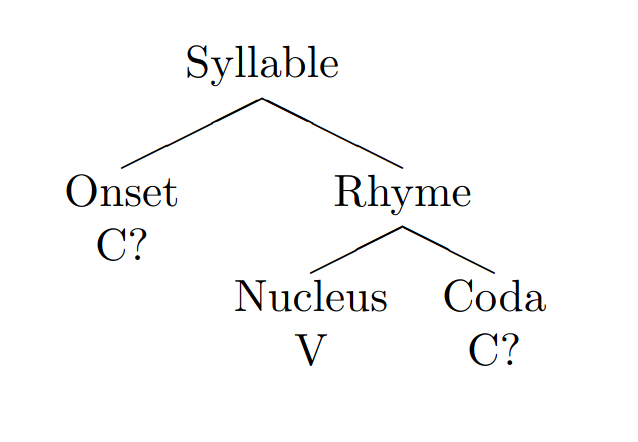
\includegraphics[width=0.6\linewidth]{syllable}
	\caption{Structure of a syllable. C-consonant, V-vowel, ?- indicates optionality}
	% \Description{Syllable structure described as a tree}
	\label{syllable}
\end{figure}


A sequence of characters that do not belong to any of the classes listed above, will not form a valid syllable and can not be accepted for pronunciation analysis. A vowel sign following an independent vowel ({\mal അി}), a word beginning with a virama ({\mal ്ക്കം}), an independent vowel after a consonant ({\mal കിഅ}) etc. are  examples of invalid sequences.




\section{The Design and Development of Mlphon}
\label{arch}

Given that Malayalam linguistic literature contains well-established pronunciation modeling rules \cite{mohanan1989syllable, asher1997, prabo2016}, we computationally model these rules in a deterministic manner using finite state transducers, which are ideal for this task \cite{kaplan1994regular}. FSTs are apt for morphological as well as phonological parsing of natural languages \cite{kaplan1994regular}. An FST maps between two sets of symbols. Formally a finite state transducer $T$ can be defined \cite{jurafsky2014speech} as a set of seven parameters ($Q,\Sigma, \Gamma, I, F, \delta, \sigma$) where

Q \textit{is a finite set of states}

$\Sigma$  \textit{is a finite set of input symbols}

$\Gamma$ \textit{is a finite set of output symbols}

I \textit{is set of initial states,  a subset of Q}

F \textit{is a set of final states,  a subset of Q}

$\delta  : Q × \Sigma → Q $ \textit{is the transition function}

$\sigma  : Q → \Gamma^* $ \textit{is the output function}


% Parsing grapheme sequence to obtain the phonemes along with their phonetic features will henceforth be referred as forward direction of parsing, and the FST performing this task will be called \emph{analysis FST}. The grapheme input to the analysis FST will be referred to as \emph{surface string} and its output, phonemes and feature tags will be referred to as \emph{analysis string}. See Fig. \ref{fstbox}, showing an example of analysis and surface strings of Phoneme Analyser FST.

\begin{figure}[h]
	\centering
	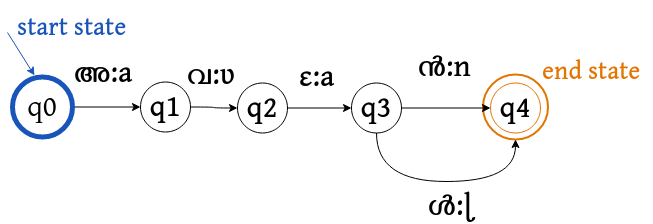
\includegraphics[width=\linewidth]{egfst.png}
	\caption{An FST representing a simple pronunciation mapping that accepts two words {\mal അവൻ} and {\mal  അവൾ}. The states are represented as circles and marked with their unique number. The initial state is represented by a bold circle and final states by double circles. An input symbol i and an output symbol o are marked on the corresponding directed arc as i : o. {\ipa ɛ} is a special symbol that indicates the generation of an output corresponding to an empty input string. Here the inherent vowel {\ipa a} is inserted at the transition from the state q2 to q3.}
% 	\Description{Analysis and Surface strings in Phoneme Analyser FST}
	\label{egfst}
\end{figure}


\begin{table}[h]
    \centering
        \caption{Parameters of FST illustrated in Fig. \ref{egfst} is defined in this table.}
    \label{fstparam}
    \begin{tabular}{c|l}
     \hline \hline
    \textbf{Parameters} & \textbf{Definition} \\ \hline
       Q  & \{{\ipa q0, q1, q2, q3, q4}\} \\
        $\Sigma$ & \{{\mal അ, വ, ൻ, ൾ}, {\ipa ɛ}\} \\
        $\Gamma$ &  \{{\ipa a, ʋ, n, ɭ}\} \\
        I & \{{\ipa q0}\} \\
        F & \{{\ipa q4}\}\\
        $\delta$ & $\delta$({\ipa q0}, {\mal അ}) = {\ipa q1}; $\delta$({\ipa q1}, {\mal വ}) = {\ipa q2}; $\delta$({\ipa q2}, {\ipa ɛ})= {\ipa q3}; \\
            & $\delta$({\ipa q3}, {\mal ൻ}) = {\ipa q4};  $\delta$({\ipa q3},{\mal ൾ}) = {\ipa q4} \\
            
        $\sigma$ & $\sigma$({\ipa q0}, {\mal അ}) = {\ipa a}; $\sigma$({\ipa q1}, {\mal വ}) = {\ipa ʋ}; $\sigma$({\ipa q2}, {\ipa ɛ})= {\ipa a}; \\
            & $\sigma$({\ipa q3}, {\mal ൻ}) = {\ipa n};  $\sigma$({\ipa q3},{\mal ൾ}) = {\ipa ɭ} \\
         \hline
      
        
    \end{tabular}

\end{table}
In an FST, every state has a finite  number of transitions to other states. An input and output symbol is used to label each transition. According to the transition function, the FST emits an output symbol for each symbol in the input string after changing its state, starting from the initial state. When it enters the final state, the FST would have accepted every symbol in the input string. The output string is made up of all the emitted symbols at that point \cite{golob2012fst}. For the cases where the number of symbols in input or output strings mismatch, a `null symbol', {\ipa ɛ} is introduced in the transition mapping. The FST described in Fig. \ref{egfst}, generates pronunciations for two words {\mal അവൻ} /{\ipa aʋan}/ and {\mal  അവൾ} /{\ipa aʋaɭ}/. Its parameters are defined in Table \ref{fstparam}.



%Formally a finite state transducer $T$ can be defined as a set of seven parameters ($Q,\Sigma, \Gamma, I, F, \delta, \sigma$) where Q = finite, non empty set of states; $\Sigma$ = finite, non empty set of input symbols; $\Gamma$ =  finite, non-empty set of output symbols; I = set of initial states, is a subset of Q; F = set of final states, is a subset of Q; $\delta$ = a transition function between the states, given a state and input string;$\sigma$ = an output function returning an output string, given a state and input string.



FSTs satisfy closure property, such that the inversion and composition of transducers are two natural consequences. According to the composition property, if transducer $T_1$ maps from input symbols $I_1$ to output symbols $O_1$ and transducer $T_2$ maps from  $O_1$ to $O_2$, then the composition $T_1 || T_2 $ maps from $I_1$ to $O_2$   \cite{jurafsky2014speech}. The composition of a series of transducers perform the mapping from an input string to output string, passing through the states defined by the constituting transducers. The inversion, $T^{-1}$ of a transducer $T$, reverses the input and output symbols. This inversion property has enabled the  development of Mlphon as a bidirectional g2p converter.


Mlphon, the tool we introduce is developed using SFST.  SFST is programming language for FSTs, written in C++ language \cite{schmid2005programming}. It has a user-friendly python API\footnote{SFST Python library: \url{https://pypi.org/project/sfst/}}, freely available under the GNU public license. SFST provides efficient mechanisms for defining the input and output symbol sets for FSTs and the rules for contextually mapping an input string to output string. SFST has been employed in the development of state of the art morphological analysers for Turkish \cite{kayabacs2019trmor}, German \cite{schmid-etal-2004-smor}, Latin \cite{springmann2016latmor}  and Malayalam \cite{thottingal-2019-finite}.

The ruleset of Mlphon can be adapted with the necessary script modifications to other Dravidian languages with a similar script nature. The rulesets and graphemes must be adjusted to fit the target language. To enable this, we have made sure the source code is accessible, well-documented, and freely licensed to allow for adaptations\footnote{https://github.com/kavyamanohar/mlphon}. In a code switching context, a language detector may be needed to separate the text and route it to language-specific g2p systems.

% According to the composition property of FST, if transducer $T_1$ maps from states $I_1$ to $O_1$ and transducer $T_2$ maps from states $O_1$ to $O_2$, then the composition $T_1 \circ T_2 $ maps from $I_1$ to $O_2$. 
% For example, the Syllabifier FST is designed as the composition of three FSTs that perform (i) normalization, (ii) word boundary tagging, and (iii) syllable boundary tagging.

% Parsing grapheme sequence to obtain the phonemes along with their closest articulatory features is referred as forward direction of parsing. The composition of a series of transducers perform the mapping from the input string to the output string, passing through the states defined by the constituting transducers.  The inversion, $T^{-1}$ of a transducer $T$, maps the output symbols of $T$ to its input symbols \cite{jurafsky2014speech}. This inversion property has enabled the  development of Mlphon as a bidirectional grapheme-phoneme converter.


\subsection{Architectural Description}


\begin{figure}[!h]
	\centering
	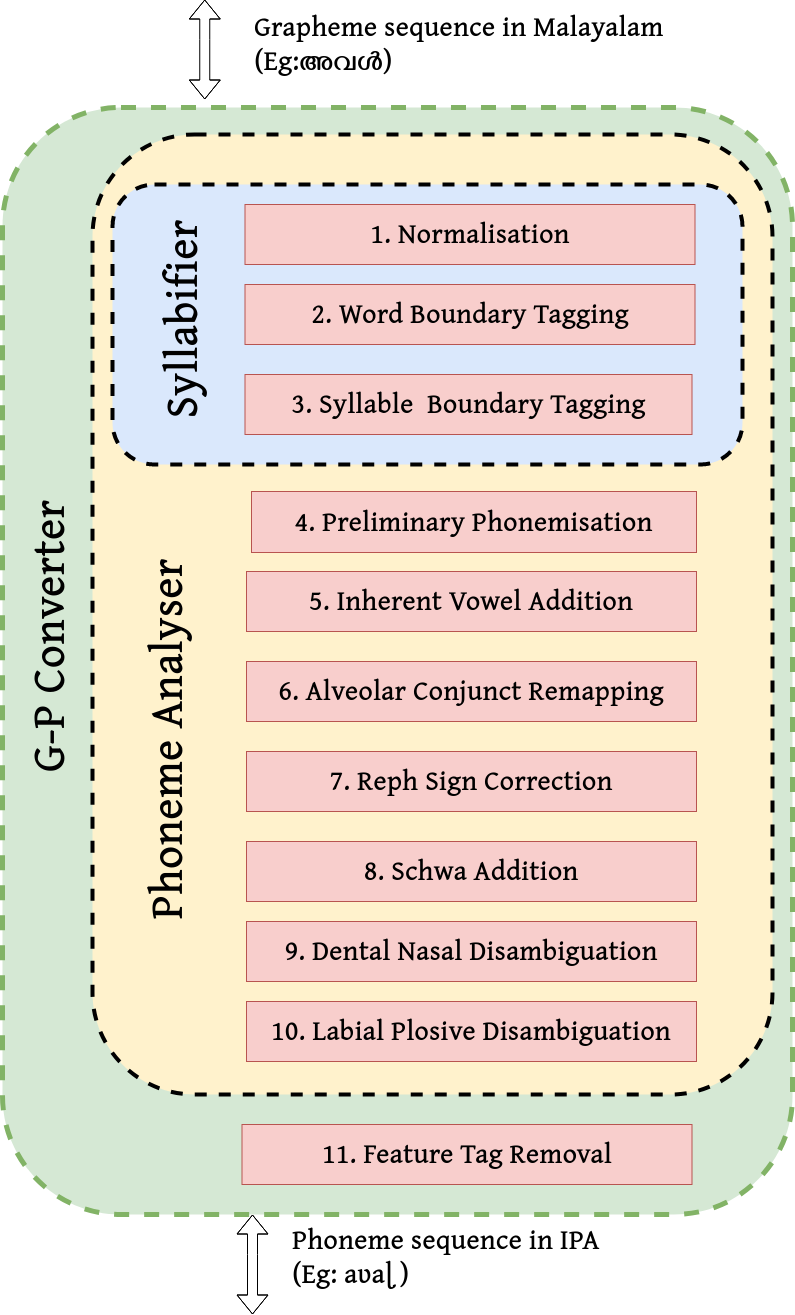
\includegraphics[width=0.9\linewidth]{g2p.png}
	\caption{The system architecture of Mlphon. Each solid rectangular box represents an FST that maps between two sets of symbols. They are composed at compile time to give final FSTs in dotted rectangular boxes. Mlphon python library provides programmable access to these final FSTs.}
	% \Description{Architecture of mlphon described as a flow graph}
	\label{architecture}
\end{figure}

The system architecture of Mlphon is described in Fig. \ref{architecture}. We follow a modular approach in the design of Mlphon. The mapping from Malayalam script to IPA is carried out in eleven steps, where each step represents an FST. In Mlphon, FST parameters are not directly defined. They are instead compiled from SFST programs. An SFST program is essentially a regular expression.  They represent context sensitive rewrite rules.  When the programs are compiled, we get eleven transducers shown in the architectural diagram in Fig. \ref{architecture}.

The SFST programs corresponding to the transducers are simplified and described in Algorithms \ref{syllabifier} - \ref{disambiguation2}. In the algorithmic description we use the SFST syntax, where {\ipa '|'} indicates the union operation, {\ipa '||'} indicates composition operation, '$\leftarrow$' indicates the mapping of the right hand side input symbol sequence to left hand side output symbol sequence. They are represented in the form:  D $\leftarrow$ [A] B [C], where B is the input  with an optional left context A and a right context C, being mapped to the output D. A, B, C, and D can represent a single symbol or a sequence of symbols. The individual symbols in a sequence is separated by a {\ipa '+'}, for enhanced readability. 

For transducers that carry out complex tasks, the expressions might be quite complicated. In order to create complex expressions from simpler ones, variables are defined \cite{schmid2005sfst}. The SFST program is structured as a combination of  (i) one-to-one and one-to-many mappings from input symbols to output symbols, (ii) contextual mappings of input symbol sequence to output symbol sequence,  and (iii) self mappings where input symbols are passed as such to the output.  Additional information is provided in comments in the algorithmic description. 
% The input and output symbols of each of these FSTs are listed in Table \ref{alphabets}. 
The individual FSTs are composed at compile time to the final FST structures namely:
 
\begin{enumerate}
    \item Syllabifier
	\item Phoneme analyser
	\item Grapheme-Phoneme (G-P) converter
\end{enumerate}

These three FSTs are bundled into Mlphon Python library along with various utility functions and released under MIT license. The programmable Python API enables its integration with many downstream NLP tasks as demonstrated in section \ref{applications}. The functionalities of the individual FSTs are described in sections \ref{normalisation} to \ref{tagremoval)}. Wherever it is essential to communicate the functionality, state transitions in each FST are diagrammatically represented.


% \begin{table*}[!h]
% \begin{center}
%     \begin{minipage}{\textwidth}

% \caption{Input and output symbols of different FSTs}    \label{alphabets}

%     			\setcounter{mpfootnote}{\value{footnote}}
% 			% Redefine the command that produces the footnote number
% 			\renewcommand{\thempfootnote}{\arabic{mpfootnote}}
% \begin{tabular}{clll}
% \hline \hline
%    No. & \textbf{FST}            & \textbf{Input Symbols, \boldmath{$\Sigma$}} & \textbf{Output Symbols, \boldmath{$\Gamma$}} \\\hline
%     1& Normalisation          & Malayalam characters                           &   \textit{Input Symbols}                          \\
%     \rowcolor{Gray}
%     2&Word Boundary Tagging   & Malayalam characters                           &  \textit{Input Symbols} , Word Tags\footnotemark[1] \\
%     3&Syllable Boundary Tagging& Malayalam characters, Word Tags      &  \textit{Input Symbols} , Syllable Tags\footnotemark[2] \\
%     \rowcolor{Gray}
%     4& Preliminary Phonemisation& Malayalam characters,Word Tags, Syllable Tags & IPA characters,  Word Tags, Syllable Tags, \\
%         \rowcolor{Gray}
%     && & Phonemic Feature Tags\footnotemark[3], Graphemic Feature Tags\footnotemark[4] \\
%     5& Inherent Vowel Addition   &  IPA characters,  Word Tags, Syllable Tags &\textit{Input Symbols}, {\ipa <inherentvowel>}  \\
%     \rowcolor{Gray}
%    6&Alveolar Conjuncts Remapping& IPA characters,  Word Tags, Syllable Tags, & \textit{Input Symbols}\\
%     \rowcolor{Gray}
%     7& Reph Sign Correction                           & Phonemic Feature Tags, Graphemic Feature Tags, &\\
%         \rowcolor{Gray}
%     &&                          {\ipa <inherentvowel>} & \\
%     8& Schwa Addition (Samvruthokaram) & IPA characters,  Word Tags, Syllable Tags, & \textit{Input Symbols}, {\ipa <schwa>}  \\
%     &&                                  Phonemic Feature Tags, Graphemic Feature Tags,& \\
%     && {\ipa <inherentvowel>}                                                       &      \\    
%            \rowcolor{Gray}
%    9& Dental Nasal Disambiguation & IPA characters,  Word Tags, Syllable Tags, & \textit{Input symbols}\\
%    \rowcolor{Gray}
%    &&                                  Phonemic Feature Tags, Graphemic Feature Tags,& \\
%   \rowcolor{Gray}
%    && {\ipa <inherentvowel>, <schwa>}                                                       &       \\  
%     10& Labial Plosive Disambiguation & IPA characters,  Word Tags, Syllable Tags, & \textit{Input Symbols}\\
%    &&                                  Phonemic Feature Tags, Graphemic Feature Tags,& \\
%    && {\ipa <inherentvowel>, <schwa>}                                                       &       \\     
%    \rowcolor{Gray}
%    11& Feature Tag Removal & IPA characters,  Word Tags, Syllable Tags, & IPA characters\\
%    \rowcolor{Gray}
%   &&                                  Phonemic Feature Tags, Graphemic Feature Tags,& \\
%    \rowcolor{Gray}
%   && {\ipa <inherentvowel><schwa>}                                                       &       \\        
%    \hline
% \end{tabular}
% 			\footnotetext[1]{{\ipa <BoW> <EoW>} }
% 			\footnotetext[2]{{\ipa <BoS> <EoS> }}
% 			\footnotetext[3]{{\ipa <velar><palatal><dental><retroflex><alveolar><labial><labiodental><plosive><voiceless><voiced><unaspirated><nasal><fricative><flapped> <aspirated><lateral><approximant><glide><trill><glottal><retroflex>}}
%    			\footnotetext[4]{{\ipa <vowel> <v\_sign> <virama><visarga><anuswara><schwa><dotreph><reph><chil> <zwj> <zwnj>} }
% 			\setcounter{footnote}{\value{mpfootnote}}

% 		\end{minipage}
% 	\end{center}
% \end{table*}

% The Mlphon python library (\url{https://pypi.org/project/mlphon/}) provides programmable access to Syllabifier, Phoneme Analyser and G-P Converter


% Table \ref{alphabets} shows the symbol set of different FSTs in Mlphon. The rules for mapping between them are defined in Algorithms \ref{syllabifier}-\ref{disambiguation2}. During compilation, the symbols and the rules get converted into FSTs with internally formulated states and transition functions. 

% \begin{figure*}[!h]
% 	\centering
% 	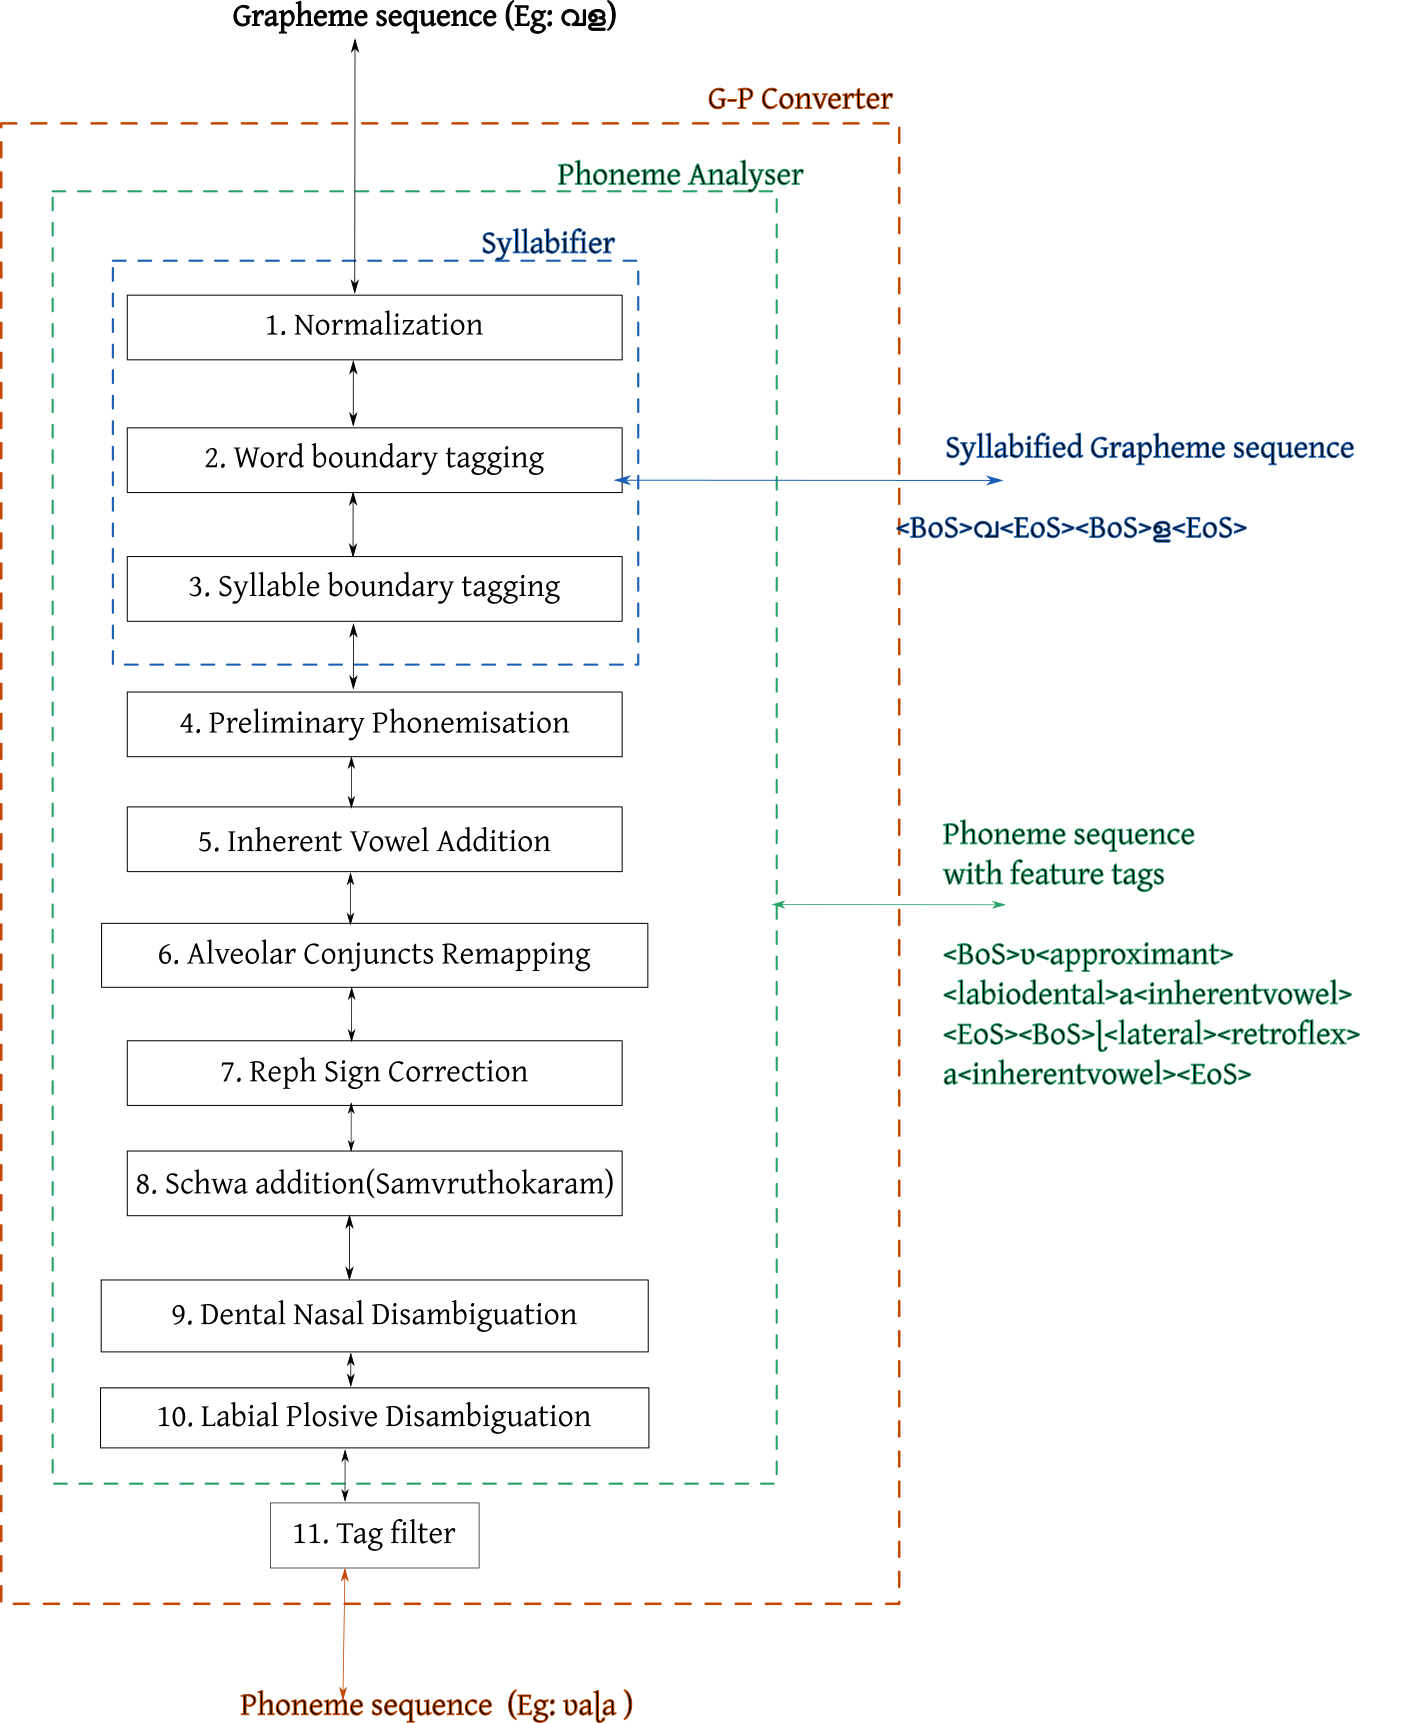
\includegraphics[width=0.9\linewidth,height=0.75\textheight]{architecture.png}
% 	\caption{The system architecture of Mlphon. Each solid rectangular box represents an FST that maps between two sets of symbols. They are composed at compile time to give final FSTs in dotted rectangular boxes. Mlphon python library provides programmable access to these final FSTs.}
% 	% \Description{Architecture of mlphon described as a flow graph}
% 	\label{architecture}
% \end{figure*}


% \begin{table*}[]
%     \centering
%         \caption{Input and output symbols of different FSTs}
%     \label{alphabets}
% \begin{tabular}{|c|l|l|}
% \hline \hline
%     \textbf{FST} & \textbf{Input Alphabets, \boldmath{$\Sigma$}} & \textbf{Output Alphabets, \boldmath{$\Gamma$}} \\\hline
%    \multirow{8}{*}{ Syllabifier} &{\mal അ ആ ഇ ഈ ഉ ഊ ഋ ൠ ഌ ൡ എ ഏ ഐ ഒ ഓ ഔ} & {\mal അ ആ ഇ ഈ ഉ ഊ ഋ ൠ ഐ ഒ ഓ ഔ}\\
%     &{\mal ാ ി ീ ൢ ൢ ു ൂ ൃ ൄ ൢ ൣ െ േ ൈ ൊ } &{\mal ാ ി ീ ൢ ൢ ു ൂ ൃ ൄ ൢ ൣ െ േ ൈ ൊ } \\
%         &{\mal ോ ൗ ൌ ം  ഃ ് ൎ} &{\mal ോ ൗ ൌ ം  ഃ ് ൎ} \\
%     &{\mal ക ഖ ഗ ഘ ങ ച ഛ ജ ഝ ഞ ട ഠ ഡ ഢ ണ }& {\mal ക ഖ ഗ ഘ ങ ച ഛ ജ ഝ ഞ ട ഠ ഡ ഢ ണ }\\
%         &{\mal  ഺ ഩ ത ഥ ദ ധ ന പ ഫ ബ ഭ മ}& {\mal ഺ ഩ ത ഥ ദ ധ ന പ ഫ ബ ഭ മ}\\
%         &{\mal  യ ര ല വ ശ ഷ സ ഹ ള ഴ റ ൺ ൻ ർ ൽ ൾ ൿ ൔ ൕ ൖ}& {\mal യ ര ല വ ശ ഷ സ ഹ ള ഴ റ ൺ ൻ ർ ൽ ൾ ൿ ൔ ൕ ൖ}\\
%         && {\ipa <BoS> <EoS>}\\
%         & \textbf{Eg Input}: {\mal വള} & \textbf{Eg Output}:  {\ipa <BoS>}{\mal വ}{\ipa <EoS>}{\ipa< BoS>} {\mal ള}{\ipa <EoS> } \\
%     \hline
%      &{\mal അ ആ ഇ ഈ ഉ ഊ ഋ ൠ ഌ ൡ എ ഏ ഐ ഒ ഓ ഔ} & {\ipa  ə
% a aː i iː u uː rɨ rɨː lɨ lɨː e eː ai̯ o oː au̯
% k kʰ ɡ ɡʱ ŋ
% t͡ʃ t͡ʃʰ ɟ ɟʱ ɲ
% }\\
    
%      &{\mal ാ ി ീ ൢ ൢ ു ൂ ൃ ൄ ൢ ൣ െ േ ൈ ൊ } &{\ipa ʈ ʈʰ ɖ ɖʱ ɳ
% t̪ t̪ʰ d̪ d̪ʱ n̪
% ṯ n
% p pʰ b bʱ m
% j ɾ l ʋ ʃ ʂ s ɦ ɭ ɻ r f} \\
    
%     & {\mal ോ ൗ ൌ ം  ഃ ് ൎ}& {\ipa <vowel> <v\_sign> <virama><visarga><anuswara> }\\
    
%         &{\mal ക ഖ ഗ ഘ ങ ച ഛ ജ ഝ ഞ ട ഠ ഡ ഢ ണ }&{\ipa <schwa><dotreph><velar><palatal><dental>} \\
%         &{\mal  ഺ ഩ ത ഥ ദ ധ ന പ ഫ ബ ഭ മ}&{\ipa <retroflex><alveolar><labial><labiodental> } \\
% Phoneme    &{\mal  യ ര ല വ ശ ഷ സ ഹ ള ഴ റ ൺ ൻ ർ ൽ ൾ ൿ ൔ ൕ ൖ}&{\ipa <plosive> <voiceless> <voiced><aspirated>} \\
%      Analyser    &&{\ipa <unaspirated><nasal><fricative><flapped> } \\
%          &&{\ipa <lateral><approximant><glide><trill>} \\
%          &&{\ipa <glottal><retroflex>} \\
%          &&{\ipa <reph><chil> <zwj> <zwnj><inherentvowel>} \\
% & \textbf{Eg Input}: {\mal വള}  & \textbf{Eg Output}: {\ipa <BoS>}{\ipa ʋ}{\ipa <approximant><labiodental>}\\
% && {\ipa a}{\ipa <inherentvowel><EoS><BoS>}{\ipa ɭ}{\ipa <lateral>}\\
% &&{\ipa <retroflex>}{\ipa a}{\ipa <inherentvowel><EoS>} \\   \hline
%         &{\mal അ ആ ഇ ഈ ഉ ഊ ഋ ൠ ഌ ൡ എ ഏ ഐ ഒ ഓ ഔ} & {\ipa  ə
% a aː i iː u uː rɨ rɨː lɨ lɨː e eː ai̯ o oː au̯
% k kʰ ɡ ɡʱ ŋ
% t͡ʃ t͡ʃʰ ɟ ɟʱ ɲ
% }\\
    
%      &{\mal ാ ി ീ ൢ ൢ ു ൂ ൃ ൄ ൢ ൣ െ േ ൈ ൊ } &{\ipa ʈ ʈʰ ɖ ɖʱ ɳ
% t̪ t̪ʰ d̪ d̪ʱ n̪
% ṯ n
% p pʰ b bʱ m
% j ɾ l ʋ ʃ ʂ s ɦ ɭ ɻ r f} \\
%   &{\mal ോ ൗ ൌ ം  ഃ ് ൎ} &\\
%   G-P  &{\mal ക ഖ ഗ ഘ ങ ച ഛ ജ ഝ ഞ ട ഠ ഡ ഢ ണ }&\\

%  Converter &{\mal  ഺ ഩ ത ഥ ദ ധ ന പ ഫ ബ ഭ മ} &\\
%   &{\mal  യ ര ല വ ശ ഷ സ ഹ ള ഴ റ ൺ ൻ ർ ൽ ൾ ൿ ൔ ൕ ൖ}&\\
% &\textbf{Eg. Input}:{\mal വള} & \textbf{ Eg. Output}: {\ipa ʋaɭa} \\


%    \hline
% \end{tabular}


% \end{table*}



%See Fig. \ref{fstbox}, showing an example of analysis and surface strings of Phoneme Analyser FST.

%\begin{figure}[h]
%	\centering
%	\includegraphics[width=0.9\linewidth]{FSTbox.pdf}
%	\caption{Analysis and Surface strings in Phoneme Analyser FST}
%	% \Description{Analysis and Surface strings in Phoneme Analyser FST}
%	\label{fstbox}
%\end{figure}



% \subsection{Syllabifier FST}
% \label{syllabification}



\begin{algorithm*}
	\caption{Normalisation, Word Boundary Tagging, Syllable Boundary Tagging}\label{syllabifier}
	\begin{algorithmic}[1]
		\Procedure{Normalisation}{}
		\State \texttt{chillunorm\_fst}: {\ipa chillu} $\gets$ {\ipa base consonant+virama+zwj} \Comment{Define a named FST for chillu normalisation}
		\State \texttt{ntanorm\_fst}: {\mal ന+്+റ} $\gets$ {\mal ൻ+്+റ}
		\State \Return \texttt{chillunorm\_fst} {\ipa  | } \texttt{ntanorm\_fst} \Comment{It is the union of two predefined FSTs}
	\EndProcedure
	\Procedure{Word Boundary Tagging}{}
		\State \Return {\ipa <BoW>+token+<EoW>} $\gets$ {\ipa token} \Comment{Insert boundary tags to input word token}
	\EndProcedure
	\Procedure{Syllable boundary tagging}{}
 		\State {\ipa c\_v} $\gets$ {\ipa consonant + virama}
   		\State {\ipa syl\_end} $=$ {\ipa [anuswara, visarga, chillu]}  \Comment{syl\_end is a variable, that can take any value in the list}
        \State \Comment{Four types of character sequences that constitute a syllable is defined in the following lines}
		\State {\ipa Type 1} $\gets$ {\ipa <BoW>+vowel+syl\_end?}  \Comment{? indicates optionaity}
		\State {\ipa Type 2} $\gets$ {\ipa consonant+vowelsign?+syl\_end?}
		\State {\ipa Type 3} $\gets$ {\ipa c\_v * + consonant} \Comment{* indicates one or more occurence}
		\State {\ipa Type 4} $\gets$ {\ipa c\_v ? + consonant + {\mal ു}? + virama + <EoW>}
		\State {\ipa syllable} $\gets$ {\ipa Type 1 | Type 2 | Type 3 | Type 4 } \Comment{A syllable is any of the 4 types}
		\State \Return {\ipa <BoS> + syllable +  <EoS>} $\gets$ {\ipa syllable} \Comment{Insert boundary tags to syllables}
	\EndProcedure
% 	\State \texttt{Syllabifier}: \texttt{Normalizer} $\circ$ \texttt{WordBoundaryTagger} $\circ$ \texttt{SyllableBoundaryTagger}
	\end{algorithmic}
\end{algorithm*}


\subsubsection{Normalisation}
\label{normalisation}

This FST accepts all Malayalam characters and invisible zero width characters\footnote{Zero Width Joiner: \url{https://en.wikipedia.org/wiki/Zero-width_joiner}}. Characters that do not require normalisation are self mapped. Character sequences that essentially represents the same graphemes are normalised to a standard form. 

\begin{figure}[h]
	\centering
	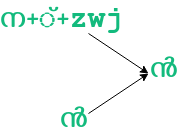
\includegraphics[width=0.4\linewidth]{norm.drawio.png}
	\caption{Two alternate representations of {\mal ൻ} at input is being mapped to the normalised form at the output}
% 	\Description{Analysis and Surface strings in Phoneme Analyser FST}
	\label{norm}
\end{figure}

Specifically this FST converts chillus represented as the sequence \texttt{base consonant},  \textit{virama} ({\mal ്}), \texttt{zwj} to atomic forms. It also converts {\mal ന്റ} {\ipa /nṯa/} represented as the sequence {\mal ൻ}, \textit{virama} ({\mal ്}), {\mal റ} to {\mal ന},  \textit{virama} ({\mal ്}), {\mal റ}. Fig. \ref{egnorm} provides an example indicating the state transitions happening in this FST. The procedural description is provided in Algorithm \ref{syllabifier}.

%The entire alphabet of Malayalam is defined as a self mapping transducer.

\begin{figure}[h]
	\centering
	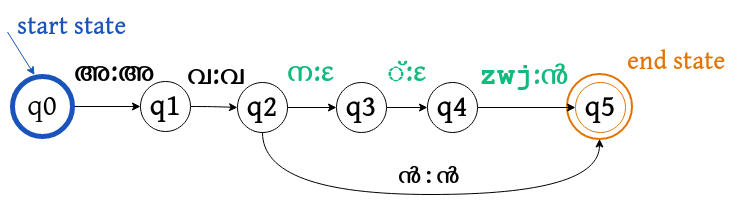
\includegraphics[width=\linewidth]{egs_norm.png}
	\caption{Normalisation of the word {\mal അവൻ}, indicating the two possible input sequences generating the normalised output. The word final \textit{chillu} grapheme represented as {\mal ന, ്,} \texttt{zwj} is normalised to a common form of single atomic character, {\mal ൻ},  by passing through states from q2 , q3, q4 and q5. If the word were already in normalized form, that character is self mapped as indicated in other transitions.}
% 	\Description{Analysis and Surface strings in Phoneme Analyser FST}
	\label{egnorm}
\end{figure}

\subsubsection{Word Boundary Tagging}

This FST accepts all Malayalam characters. The token passed to Mlphon for analysis is considered as a word. Tags in angle brackets {\ipa <BoW>} and {\ipa <EoW>} are added to indicate the beginning of word and the end of word respectively by this FST and is returned to the output. The procedural description is provided in Algorithm \ref{syllabifier}.

\subsubsection{Syllable Boundary Tagging}
\label{syllabletagger}


\begin{figure}[h]
	\centering
	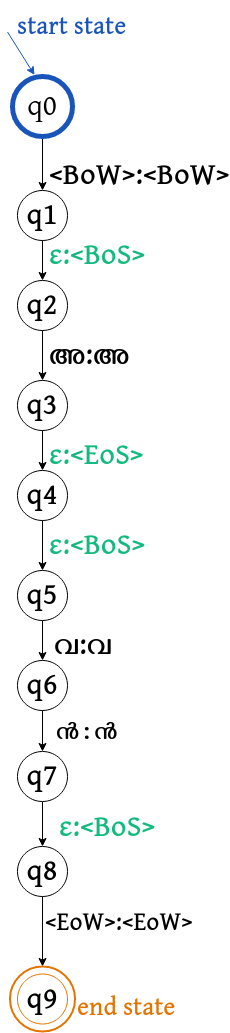
\includegraphics[width=0.25\linewidth]{egs_syltags.png}
	\caption{Insertion of syllable tags, {\ipa <BoS> <EoS>} are indicated by transitions in green colour. All other symbols are mapped to themselves. Word boundary tags inserted in previous FST is also shown. }
% 	\Description{Analysis and Surface strings in Phoneme Analyser FST}
	\label{egs_syltags}
\end{figure}
This FST accepts all Malayalam characters, along with word boundary tags. As discussed in section  \ref{syllablestructure}, some character sequences are invalid according to Malayalam script grammar. The syllabifier FST checks for validity of character sequences to form syllables.  An invalid sequence of Malayalam characters will  not find a path from the start state of this FST to the end state and will summarily be rejected. On valid input strings, it inserts tags - {\ipa <BoS>}, {\ipa <EoS>} - at appropriate positions to indicate the beginning and end of the syllables. The syllable boundary tags are essential for pronunciation analysis. This procedure is explained in Algorithm \ref{syllabifier}. An example for the insertion of syllable tags is indicated in Fig. \ref{egs_syltags}.


\subsubsection{Preliminary Phonemisation}


This FST accepts valid sequence of Malayalam characters separated by word and syllable boundary tags. The transitions defined by this FST maps every grapheme to phonemes as per tables \ref{vowelgrapheme}-\ref{chillus} along with phonetic or graphemic feature tags. 
% The list of these tags are available in Table \ref{alphabets}. 
The preliminary mapping carried out by this FST will be modified by subsequent FSTs based on contexts. The boundary tags are self mapped, so that they will be retained as such in the output. An example of mapping the graphemes {\mal സ} and {\mal മ} to its phoneme with phonetic features is described in Algorithm \ref{tagging}.





% The preliminary mapping of graphemes , are performed by this FST. During this mapping,  phonetic feature tags are added to each  phoneme.
% , and vowel phonemes are associated with tags indicating their graphemic origin (independent vowel or vowel sign).
% Once word and syllable boundary tags are inserted, the next task is to map each grapheme to phoneme. This is done as per the mapping listed in Tables  .  Inherent vowels and effect of virama on phonemes will be mapped only in the subsequent stages.

\begin{algorithm}
	\caption{Preliminary Phonemisation}\label{tagging}
	\begin{algorithmic}[1]
	\Procedure{Preliminary Phonemisation}{}
		\State \texttt{g2p\_1}: {\ipa s+<fricative>+<alveolar>} $\gets$ {\mal സ}
		\State  \texttt{g2p\_2}: {\ipa m+<labial>+<nasal>} $\gets$ {\mal മ} 
		\State ...
		\State ... \Comment Basic g2p mappings
		\State \Return \texttt{g2p\_1} $||$ \texttt{g2p\_1} . . . 
  \State \Comment Composition of basic g2p mappings
	\EndProcedure
	\end{algorithmic}
\end{algorithm}

\begin{algorithm*}
	\caption{Inherent Vowel Addition, Alveolar Conjuncts Remapping and Reph Sign Correction}\label{disambiguation}
	\begin{algorithmic}[1]
	\Procedure{Inherent Vowel Addition}{}
        \State {\ipa pre\_context} $=$ {\ipa consonant+<tags>} \Comment{Define a variable that is a sequence of consonants and tags}
		\State {\ipa post\_context} $=$ {\ipa [<chil>, <anuswara>, <visarga>, <EoS>]} \Comment{Define a variable that takes any value in the list}
		\State \Return {\ipa [pre\_context]} {\ipa a+<inherentvowel>} {\ipa [post\_context]} $\gets$ {\ipa [pre\_context]}  {\ipa ɛ } {\ipa [post\_context]}
	\EndProcedure  \Comment <tags> - represent the sequence of phonetic feature tags
		\Procedure{Alveolar conjuncts remapping}{}
		\State \texttt{tta\_fst}: {\ipa [<BoS>,<virama>]+ṯ+<tags>+ṯ+<tags>} $\gets$ {\ipa [<BoS>,<virama>]+r+<tags>+r+<tags>}
		\State \texttt{nta\_fst}: {\ipa <BoS>+n̪+<tags>+ṯ+<tags>} $\gets$ {\ipa <BoS>+n+<tags>+r+<tags>}
		\State \Return \texttt{tta\_fst $||$ nta\_fst} \Comment{Composition of two FSTs}
		\EndProcedure
	\Procedure{Reph Sign Correction}{}
		\State \Return {\ipa [ɡ,d̪]+<tags>+<virama>+ɾ+<flapped>+<reph>} $\gets$ {\ipa [ɡ,d̪]+<tags>+<virama>+r+<trill>+<reph>}
	\EndProcedure
	\end{algorithmic}
\end{algorithm*}


\subsubsection{Inherent Vowel Addition}

Inherent vowel {\ipa /a/} is added after consonant phonemes if it is at the end of a syllable position, or it is followed by the \textit{anuswara}, \textit{visarga}, or a \textit{chillu} as described in Algorithm \ref{disambiguation}.



\subsubsection{Alveolar Conjuncts Remapping}

The most common alveolar consonant clusters in Malayalam, {\mal ന്റ} {\ipa /nṯa/} and {\mal റ്റ} {\ipa /ṯṯa/} are constituted from consonants dental nasal {\mal ന} /{\ipa n̪a/} and alveolar trill {\mal റ} {\ipa /ra/}, the pronunciations of which are strikingly different. Thus the grapheme sequence {\mal ന} {\ipa /n̪a/}, \textit{virama}, {\mal റ} {\ipa /ra/} can  be mapped to {\ipa /nṯa/} instead of {\ipa /n̪ra/}. Also the grapheme sequence {\mal റ} {\ipa /ra/}, \textit{virama}, {\mal റ} {\ipa /ra/} can  be mapped to {\ipa /ṯṯa/} instead of {\ipa /rra/}. This unambiguous mapping is done by an FST  that checks the context and remaps these phonemes as indicated in Algorithm \ref{disambiguation}.

\subsubsection{Reph Sign Correction}

If the final consonant in a cluster is the alveolar tap {\mal ര} {\ipa /ɾa/}, its pronunciation gets modified to {\mal റ} {\ipa /ra/} depending on the preceding consonants. The  {\mal ര}  {\ipa /ɾa/} sound is retained only if the preceding consonant of the cluster is voiced velar or dental plosive ({\mal ഗ} {\ipa /ga/} or {\mal ദ} {\ipa /d̪a/}) as described in Algorithm \ref{disambiguation}.


\subsubsection{Schwa Addition (\textit{Samvruthokaram})}

\textit{Samvruthokaram} is a unique feature of Malayalam. Whenever there are consonants followed by \textit{virama} at word ends, a half-u sound of mid-central vowel schwa is added at word end as described in Algorithm \ref{disambiguation2}. This FST basically disambiguates the function of \textit{virama}. Loan words get adapted to native pronunciation by schwa addition at word ends. eg: {\mal ബാങ്ക്} {\ipa /baːŋkə/} (\textit{bank)}


% But there are non-native proper names, derived from Sanskrit or other foreign language, that end in virama, but pronunciation involves no schwa. eg: ജോർജ്, സന്തോഷ്, രാജീവ്, ജോസ്


\subsubsection{Dental Nasal Disambiguation}

% As already discussed in Section \ref{consonantg2p}, the alveolar nasal grapheme {\mal ഩ} {\ipa /na/}, is not widely used in Malayalam except in the context of grammatical discussions. 
The dental nasal grapheme {\mal ന} {\ipa /n̪a/}, is pronounced as the alveolar nasal {\ipa /na/} in the following  contexts\cite{prabo2016}:
% and is mostly in unambiguous distribution in native Malayalam morphemes. The contexts in which {\mal ന} {\ipa /n̪a/} takes alveolar {\ipa /na/} pronunciation 


\begin{enumerate}
	\item When a morpheme medial syllable starts in {\mal ന} and is followed by a vowel sound.

	      eg: {\mal ആന} {\ipa /aːna/} (\textit{elephant}), {\mal ഗാനം} {\ipa /ɡaːnam/} (\textit{song}), {\mal അനുജൻ} {\ipa /anuɟan/} (\textit{younger brother})
	\item When {\mal ന} is the starting character in a consonant cluster followed by {\mal യ} {\ipa /ja/}, {\mal വ}  {\ipa /ʋa/} or {\mal മ} {\ipa /ma/}.

	      eg: {\mal നന്മ} {\ipa /n̪anma/} (\textit{virtue}), {\mal ന്യായം} {\ipa /njaːjam/} (\textit{justice}), {\mal അന്വേഷണം} {\ipa /anʋeːʂaɳam/ }(\textit{enquiry})
	\item When {\mal ന} is the second character in a consonant cluster, beginning with {\mal ക} {\ipa /ka/}, {\mal ഘ} {\ipa /ɡʱa/}, {\mal പ} {\ipa /pa/}, {\mal മ} {\ipa /ma/}, {\mal ശ} {\ipa /ʃa/} and {\mal സ} {\ipa /sa/}.

	      eg: {\mal വിഘ്നം} {\ipa /ʋiɡʱnam/} (\textit{blockage}) , {\mal സ്വപ്നം} {\ipa /sʋapnam/} (\textit{dream}), {\mal പ്രശ്നം} {\ipa /praʃnam/} (\textit{issue}), {\mal സ്നേഹം} {\ipa /sneːɦam/} (\textit{love})

\end{enumerate}

These three rules are implemented by identifying the context of appearance of {\mal ന} in terms of the surrounding consonants and syllable boundaries etc. as described in the Algorithm \ref{disambiguation2}.


%
%As the tool can not detect presence of multiple morphemes from a morphologically complex word, word-medial morpheme beginning with {\mal ന} will be identified as {\ipa n<nasal><alveolar>} instead of {\ipa n̪<nasal><dental>} as in the transcription of {\mal സേവ\textbf{നാ}ഴി} {\ipa /seːʋanaːɻi/}. The percentage of failures it can cause in g2p mapping is analysed in the evaluation section.
%  The second and third rules describe how to pronounce {\mal ന} when it occurs in consonant clusters. It depends on the preceding or succeeding consonants in the clusters and the distribution is unambiguous.

% When {\mal ന} is geminated, grapheme context and the morphological composition determines the pronunciation. For example, {\mal എന്നാൽ} has two different morphological analysis possible. When it is the instrumental inflection on first person singular in Malayalam, it should be phoneme mapped to {\ipa /ennal/}. When the same word has an alternate usage as `but', its phoneme mapping should be  {\ipa /en̪n̪al/}. Such words are assigned with two possible phonemic mappings. These rules are insufficient to handle loan words and morphologically complex words and causes phoneme transcription errors discussed in Section \ref{goldlexicon}.




%\begin{lstlisting}[frame=tb, language=python, caption= Python script for grapheme to phoneme conversion, label ={g2ppython}]
%	from mlphon import PhoneticAnalyser
%	mlphon = PhoneticAnalyser()
%	print(mlphon.grapheme_to_phoneme('@{\mal വള}@'))
%	print(mlphon.grapheme_to_phoneme('@{\mal അവൻ}@'))
%	['@{\ipa ʋaɭa}@']
%	['@{\ipa aʋan}@']
%\end{lstlisting}




\subsubsection{Labial Plosive Disambiguation}
\label{labiodentalfricative}

The unvoiced aspirated labial plosive grapheme {\mal ഫ} {\ipa /pʰa/} is used to represent the labiodental fricative {\ipa /f/} in non-native words. On analysing a corpus of 100k most frequent Malayalam words  \cite{kunchukuttan2020ai4bharat}, only 6\% of words that contained the letter  {\mal ഫ} were native. All those native words had the letter  {\mal ഫ}, either preceded by the letter  {\mal സ്} or followed by {\mal ല}.  This graphemic context is used as the parameter to determine the word origin and remap fricative to plosive as described in Algorithm \ref{disambiguation2}.



% Native words with {\mal ഫ} /pʰ/: {\mal ഫലം} {\ipa /pʰalam/} (\textit{fruit}), {\mal ഫലിതം} {\ipa /pʰalit̪am/} (\textit{joke}), {\mal സ്ഫടികം} {\ipa /spʰaʈikam/} (\textit{glass}) . Non-native words with {\mal ഫ} {\ipa /f/}: {\mal ഫാൻ} {\ipa /faːn/}(\textit{fan}) , {\mal ഫോൺ} {\ipa /foːɳ/} (\textit{phone}), {\mal ഫാക്ടറി} {\ipa /faːkʈari/} (\textit{factory}), {\mal ഫാസ്റ്റ്} {\ipa /faːsṯ/ }(\textit{fast}), {\mal ഫാഷൻ} {\ipa /faːʂan/} (\textit{fashion}), {\mal ഇൻഫർമേഷൻ} {\ipa /infarmeːʂan/} (\textit{information}).

% \subsubsection{Phoneme Sequence with Feature Tags}

% The sequence of transducers described above is composed into a single large FST during compile time. Fig. \ref{phanalysissfst} illustrates the state transitions and the insersion of tags in the phoneme analyser FST when input tokens passed are: {\mal വള} and {\mal അവൻ}. The python interface of Mlphon utilizes this FST to phonemically analyse the Malayalam word and return the sequence of phonemes and feature tags. If the token {\mal അവൻ } is passed to the phoneme analyser FST, it returns the string  {\ipa <BoS>a<vowel><EoS><BoS>ʋ<approximant><labiodental>a <inherentvowel>n<chil><EoS>}.

% A tag parser function in the python interface can return the IPA and anaysis tags.



\subsubsection{Feature Tag Removal}
\label{tagremoval)}

The tag-removal FST  removes the boundary tags and phonetic feature tags, by mapping them to the null symbol {\ipa ɛ}. It will leave just the IPA symbols at the output.



\begin{algorithm*}[h]
	\caption{Schwa Addition, Dental Nasal Disambiguation,  Labial Plosive Disambiguation}\label{disambiguation2}
	\begin{algorithmic}[1]
	\Procedure{Schwa Addition}{}
		\State \texttt{schwa\_1}: {\ipa ə+<schwa>+<EoS>} $\gets$ {\ipa u+<v\_sign>+<virama>+<EoS>} \Comment{Define named FSTs for schwa addition}
		\State \texttt{schwa\_2}: {\ipa ə+<schwa>+<EoS>} $\gets$ {\ipa <virama>+<EoS>} 
		\State \Return \texttt{schwa\_1} $||$ \texttt{schwa\_2} \Comment{Return the composition of two FSTs}
	\EndProcedure
	\Procedure{Dental Nasal Disambiguation}{}
		\State \texttt{nasalrule\_1}:
		{\ipa <BoS>+n+<alveolar+<virama>+[j,ʋ,m]} $\gets$ {\ipa <BoS>+n̪<dental+<virama>+[j,ʋ,m]} \Comment{Define named FSTs}
		\State \texttt{nasalrule\_2}:
		{\ipa <EoS>+<BoS>+n<alveolar>+[vowel]} $\gets$ {\ipa <EoS>+<BoS>+n̪+<dental+[vowel]}
		\State \texttt{nasalrule\_3}: {\ipa [k,ɡʱ,p,m,ʃ,s]+<tags>+<virama>n<alveolar>} $\gets$ {\ipa [k,ɡʱ,p,m,ʃ,s]+<tags>+<virama>n̪<dental>}
		\State \Return \texttt{nasalrule\_1 $||$ nasalrule\_2 $||$ nasalrule\_3} \Comment{Return the composition of three FSTs}
	\EndProcedure
	\Procedure{Labial Plosive Disambiguation}{}
		\State \texttt{fa\_1}: {\ipa <BoW>+<BoS>+pʰ<plosive>+a+<EoS>+<EoW>} $\gets$ {\ipa <BoW>+<BoS>+f<fricative>>+a+<EoS>+<EoW>}
		\State \texttt{fa\_2}: {\ipa s+<fricative>+<alveolar>+<virama>+pʰ+<plosive>} $\gets$ {\ipa s+<fricative>+<alveolar>+<virama>+f<fricative>}
		\State \texttt{fa\_3}: {\ipa pʰ<plosive>+a+<EoS>+<BoS>+l} $\gets$ {\ipa f<fricative>+a+<EoS>+<BoS>+l}
		\State \Return \texttt{fa\_1 $||$ fa\_2 $||$ fa\_3} \Comment{Return the composition of three FSTs}
	\EndProcedure
	\end{algorithmic}
\end{algorithm*}


\subsection{Syllabifier FST}
\label{syllabification}

The composition of the series of FSTs from \ref{normalisation} to \ref{syllabletagger} results in a very useful module that performs syllabification of Malayalam text. We compose these FSTs to get the Syllabifier FST and provide programmable access to it in the Mlphon Python library. This module has interesting applications like developing subword level language modeling for ASR as described in section \ref{applications}. An illustration of this module accepting Malayalam text as input and generating output with syllable boundary tags is shown in Fig. \ref{syllabifierblock}.


\begin{figure}[h]
	\centering
	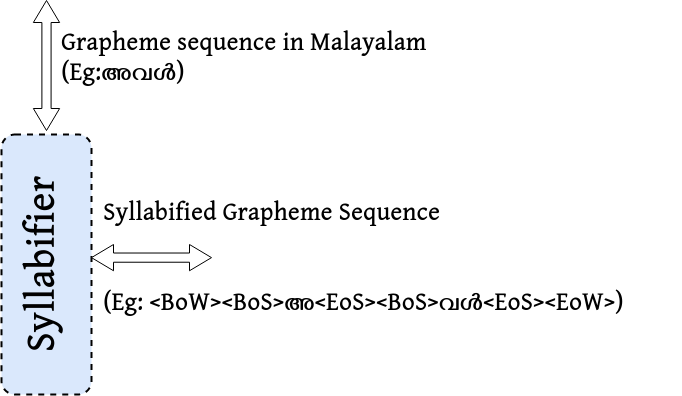
\includegraphics[width=0.8\linewidth]{syllabifier.png}
	\caption{Syllabifier performing syllabification on the word {\mal അവൾ}. Boundary tags for words and syllables are demonstrated.}
	% \Description{State Transition diagram of FST for syllabification}
	\label{syllabifierblock}
\end{figure}

% \begin{figure*}[!h]
% 	\centering
% 	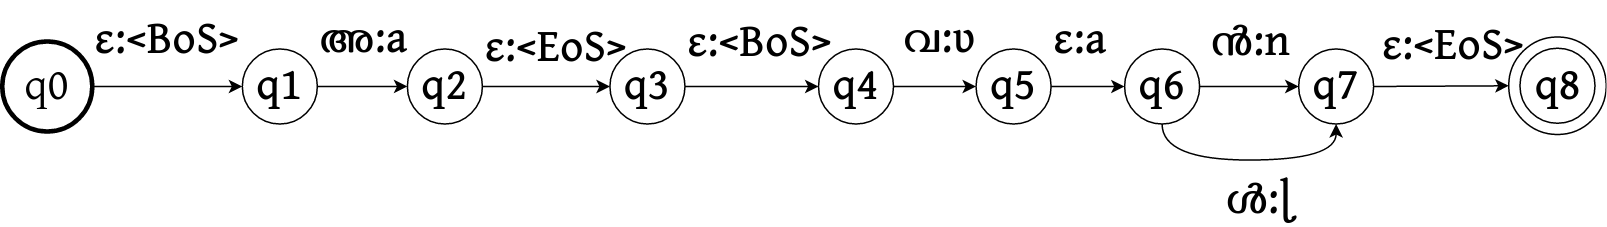
\includegraphics[width=0.9\linewidth]{syllable-drawio.png}
% 	\caption{State transitions in syllabifier FST, when the input words are  {\mal അവൻ} and {\mal അവൾ}. }
% 	% \Description{State Transition diagram of FST for syllabification}
% 	\label{sylfst}
% \end{figure*}


% Fig. \ref{sylfst} illustrates the state transitions and the insertion of tags in the syllabifier FST when input tokens passed are: {\mal അവൾ} and {\mal അവൻ}. Note that {\ipa ε} indicate the empty transition string. 
If the token passed to the syllabifier is {\mal അവൾ}, it returns the syllabified string  {\ipa <BoS>}{\mal അ}{\ipa <EoS><BoS>}{\mal വൾ}{\ipa <EoS>}.  The python interface to the FST for syllabification, parses the boundary tags and returns the sequence of syllables.
% as shown in the Listing \ref{pythonsyllabification}.





%\begin{lstlisting}[frame=tb,language=python,caption= Python script for phoneme to grapheme conversion, label={p2gpython}]
%	from mlphon import PhoneticAnalyser
%	mlphon = PhoneticAnalyser()
%	print(mlphon.phoneme_to_grapheme('@{\ipa ʋaɭa}@'))
%	print(mlphon.phoneme_to_grapheme('@{\ipa aʋan}@'))
%	['@{\mal വള}@']
%	['@{\mal അവൻ}@']
%\end{lstlisting}


\subsection{Phoneme Analyser FST}

Phoneme analyser FST is compiled as a composition of 10 FSTs described in  sections \ref{normalisation} to \ref{labiodentalfricative} and indicated in Fig. \ref{architecture} of Mlphon architecture. This FST accepts a grapheme sequence as input and returns phoneme sequence, tagged with their phonetic features.  If the token {\mal അവൾ } is passed to the phoneme analyser FST, it returns the string  {\ipa <BoS>a<vowel><EoS><BoS>ʋ<approximant><labiodental>a
<inherentvowel>ɭ<chil><EoS>} as illustrated in Fig. \ref{analysisblock}. This module can play crucial role in the context of linguistic learning providing pronunciation information regarding the graphemes in a word.


% Its operation as the composition of different FSTs is explained in the following subsections.
% The sequence of transducers  is composed into a single large FST during compile time. 
\begin{figure}[h]
	\centering
	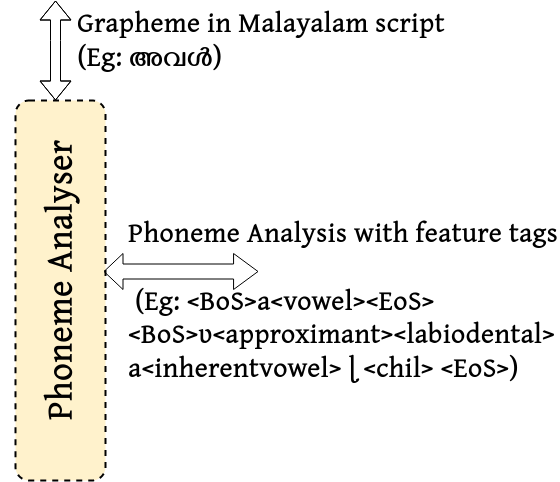
\includegraphics[width=0.6\linewidth]{analysisbox-drawio.png}
	\caption{Phoneme analyser performing analysis on the word {\mal അവൾ}. It returns the sequence of phonemes in its pronunciation along with articulatory feature tags in angle brackets.}
	% \Description{State Transition diagram of FST for syllabification}
	\label{analysisblock}
\end{figure}



Fig. \ref{phanalysissfst} illustrates the state transitions and the insertion of tags in the phoneme analyser FST when input tokens passed are: {\mal അവൾ} and {\mal അവൻ}. The python interface of Mlphon utilizes this FST to  analyse the Malayalam word and return the sequence of phonemes and phonetic feature tags like place and manner of articulation.


\begin{figure}[!h]
	\centering
	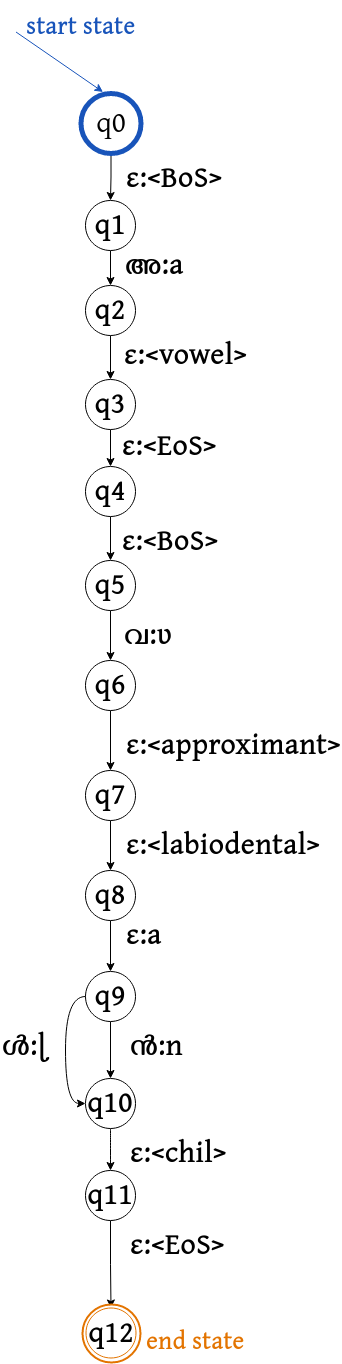
\includegraphics[scale=0.25]{analysis-dawio.png}
	\caption{Phoneme analyser FST, showcasing grapheme to phoneme conversion on the word {\mal അവൾ}.}
	% \Description{State Transition diagram of FST for phoneme analysis}
	\label{phanalysissfst}
\end{figure}

\subsection{G-P Converter FST}

A transducer that takes in a grapheme sequence and gives out its pronunciation as IPA in analysis mode and does the reverse in generate mode is the bidirectional grapheme-phoneme converter FST. It is marked as G-P converter in Fig. \ref{architecture}. All the FSTs previously discussed are bidirectional. However the bidirectionality property is particularly useful when there is need to convert graphemes to phonemes and vice-versa. Fig. \ref{gpconverterfst} demonstrates an  input and output symbol sequence of G-P Converter FST.


\begin{figure}[!h]
	\centering
	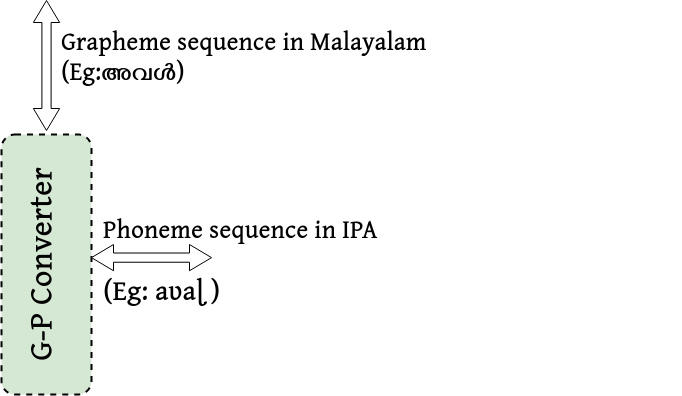
\includegraphics[scale=0.25]{g-pconverter-drawio.png}
	\caption{G-P Converter FST, performing phoneme analysis on the word {\mal അവൾ}.}
	% \Description{State Transition diagram of FST for phoneme analysis}
	\label{gpconverterfst}
\end{figure}


This FST, parses the words {\mal അവൾ} and {\mal അവൻ} in analysis mode as shown in the Fig. \ref{g2pfst} (i). When operated in generate mode, it  converts a valid phoneme sequence into graphemes. For example, in generate mode, it can parse the inputs {\ipa aʋaɭ} and {\ipa aʋan} as shown in Fig. \ref{g2pfst} (ii).

\begin{figure}[h]
	\centering
	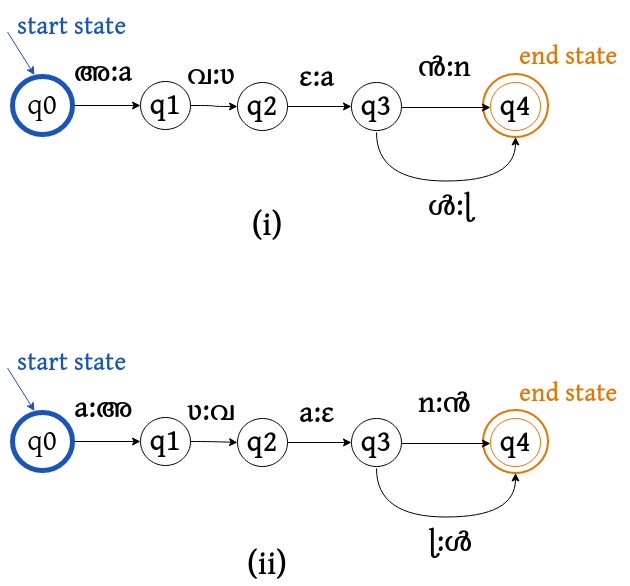
\includegraphics[width=0.75\linewidth]{g2p-fst-drawio.png}
	\caption{G-P converter FST performing (i) grapheme to phoneme conversion on the words  {\mal അവൾ} and {\mal അവൻ} in analysis mode and (ii) phoneme to grapheme conversion on {\ipa aʋaɭ} and {\ipa aʋan} in generate mode. }
	% \Description{State Transition diagram of FST for g2p}
	\label{g2pfst}
\end{figure}


% \begin{figure}[h]
% 	\centering
% 	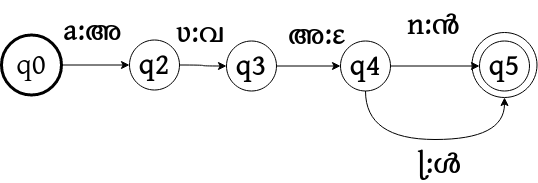
\includegraphics[width=0.7\linewidth]{p2g-fst-drawio.png}
% 	\caption{G-P FST, performing phoneme to grapheme conversion on {\ipa aʋaɭ} and {\ipa aʋan} in generate mode }
% 	% \Description{State Transition diagram of FST for p2g}
% 	\label{p2gfst}
% \end{figure}
% The python script utilizing Mlphon library to perform grapheme to phoneme and the reverse operations are illustrated in Listings \ref{g2ppython} and \ref{p2gpython}.

\subsection{The Python Library: Mlphon}
\label{pypi}
The core functionalities of Mlphon is written in SFST and compiled into different finite state transducers. SFST compiles the rules to form minimized FSTs which are very much memory optimized \cite{mohri-1997-finite}. The python binding of SFST provides access to these transducers for high level programming. Mlphon python library is very compact with 21 kB of total file size.

One of the major motivation behind this work is to provide pronunciation lexicon  for integrating with ASR and TTS applications. The pronunciation lexicon may require the transcriptions to have delimiters between phonemes and/or syllables depending on the application. The utility functions \texttt{split\_as\_phonemes} and \texttt{split\_as\_syllables} provided with Mlphon python library can parse the phonemic analysis to a sequence of phonemes or sequence of syllables separated by spaces.  Additionally the function \texttt{phonemise} accepts the delimiters defined by the user to separate phonemes and syllables.

The Mlphon library also provides a command line utility for the tasks of syllabification, phoneme analysis and conversion between graphemes and phonemes.
See Listing \ref{cli} for its usage and the list of optional arguments.
The entire development process was guided by a set of unit tests to ensure expected functionalities.

\begin{lstlisting}[frame=tb,
	caption= Command line utility for Mlphon library,
	label={cli}
%	basicstyle=\footnotesize
	]
mlphon [-h][-s][-a][-p][-g][-i INFILE][-o OUTFILE][-v]

optional arguments:
-h,--help 
-s,--syllabify
-a,--analyse
-p,--tophoneme
-g,--tographeme
-i INFILE,--input INFILE	
-o OUTFILE,--output OUTFILE	
-v, --verbose
\end{lstlisting}

\section{Intrinsic Evaluations and Discussions}
\label{goldlexicon}

Evaluating a script analysis toolkit like Mlphon is not straight forward due the absence of any baseline ground truth linguistic resource. A gold standard with manually annotated data, which can serve as a reference is an important part of any quantifiable evaluation \cite{kayabacs2019trmor}. A gold standard for g2p conversion contains a list of words annotated with their true phoneme transcription. A gold standard for syllabifier is annotated as a sequence of syllables. If a word has multiple possible annotations, all of those should be present in the gold standard lexicon. Before we explain the evaluation, the following section presents the design of gold standard lexicon. It follows a similar procedure and the number of entries as in \cite{kayabacs2019trmor}, used for creating a gold standard annotations for Turkish morphological analyser.

\subsection{Design of Gold Standard Lexicon}

The lexical entries in gold standard lexicon are chosen from the IndicNLP Corpus\footnote{\url{https://github.com/AI4Bharat/indicnlp_corpus}} \cite{kunchukuttan2020ai4bharat} which is a list of words with frequency information. These words belong to a general domain, web crawled Malayalam text corpus of 167.4 million tokens with 8.8 million types. 

The manually verified gold standard annotations were created semi-automatically. The process began with the syllabification of 1000 of the most common words in this corpus using Mlphon. It gave back a list of words, some of which had the proper syllabification and others of which had none at all. A small portion of the words that couldn't be syllabified were incorrectly spelled, which is typical of a corpus compiled from web crawls. Misspelt words were manually corrected in the corpus and syllabified. All the syllabifications performed by Mlphon were also manually verified and corrected by expert linguists, if found to be wrong. For the remaining words, which could not be syllabified, manual annotation was performed. Thus the gold standard lexicon for syllabification was obtained.

The gold standard lexicon for g2p mapping followed a similar procedure. Mlphon was used to phoneme map the spelling corrected 1000 words. The returned results were manually corrected for deletion, substitution and insertion errors. The manual corrections were performed, following all the rules and descriptions in the reference books \cite{asher1997,prabo2016}. The removal of word final schwa (\textit{samvruthokaram}) in proper nouns was suggested in a consultation with linguists. The final annotations on the gold standard lexicon were approved by them.

\begin{figure}[h]
    \centering
    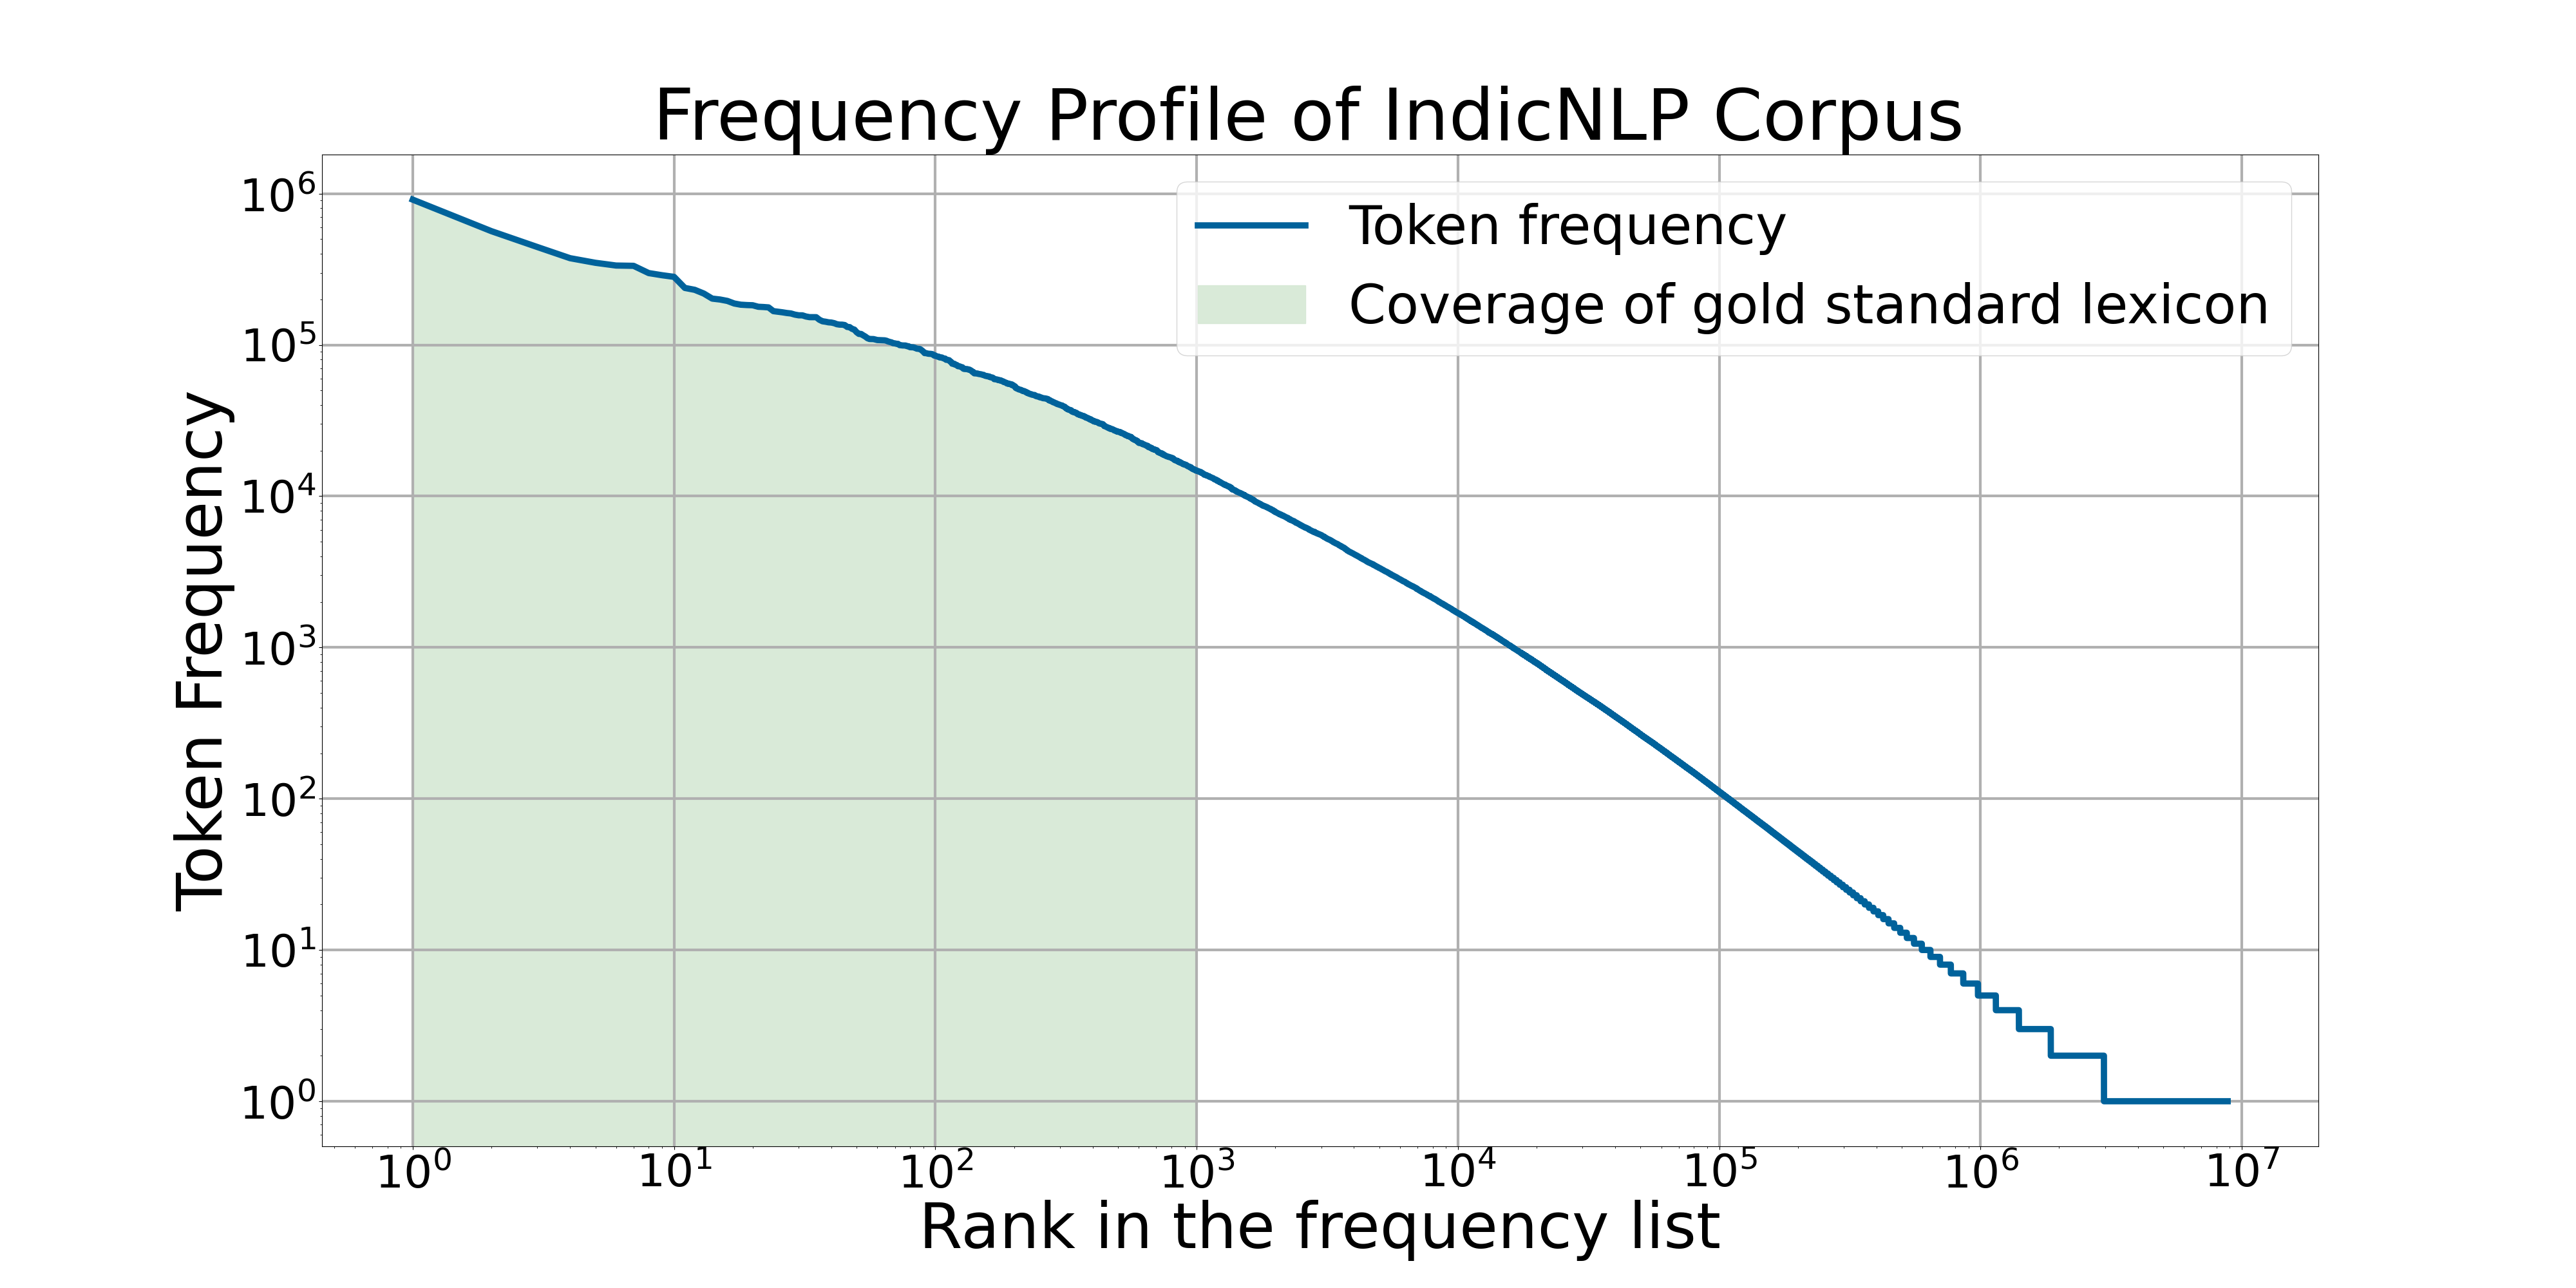
\includegraphics[width=\linewidth]{rank.png}
    \caption{The lexical entries of gold standard lexicon is chosen from the most frequent thousand words from the IndicNLP corpus \cite{kunchukuttan2020ai4bharat} such that these words cover 26\% of the 167.4 million tokens present in this corpus.}
    \label{rank}
    % Code Location: /home/kavya/researchdev/raw/
\end{figure}



The lexical entries in the gold standard lexicon constitutes  26\% of the total number of tokens in the said corpus according to the computation shown in (\ref{coverage-calc}). The frequency profile in Fig. \ref{rank} illustrates this. The coverage of tokens in the gold standard lexicon with respect to the corpus is computed as: 

\begin{equation}
\label{coverage-calc}
\begin{split}
Coverage & =\frac{\sum{}{}{Frequency\ of\ top\ 1000\ tokens} \times 100 }{Total\ token\ count\ in\ corpus}  \\ \\
&  \approx \frac{44321494 \times 100}{167.4\ million} \\ \\
& \approx 26 \%
\end{split}
\end{equation}
 The gold standard lexicon covers many regular words, loan words, proper nouns and abbreviations as per the distribution illustrated in Fig. \ref{pie-chart}. 



\begin{figure}[h]
    \centering
    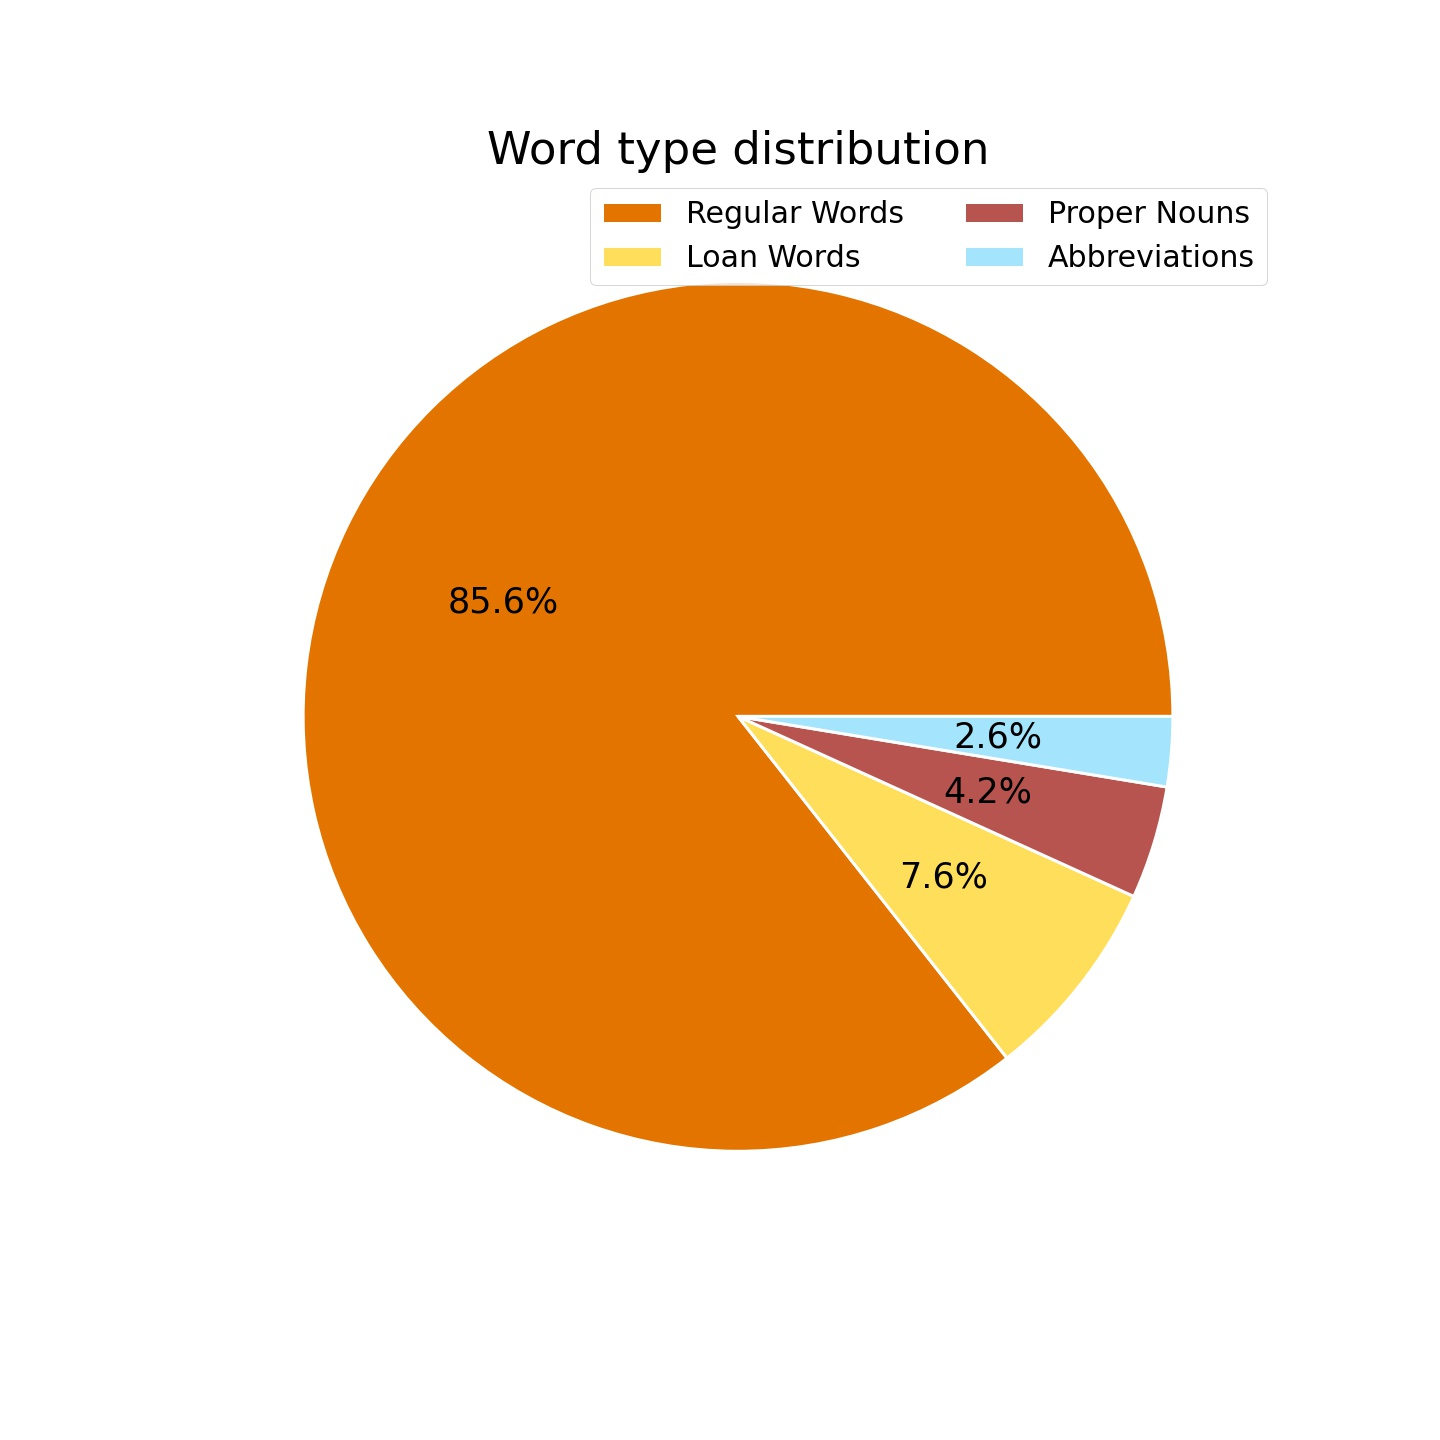
\includegraphics[trim={3cm 8cm 3cm 0cm},clip=true, width=\linewidth]{wordtypes.jpg}
    \caption{Distribution of word types in gold standard lexicon}
    \label{pie-chart}
    % Data Location: /home/kavya/tmp/phonemes/
\end{figure}


\begin{figure}[h]
    \centering
    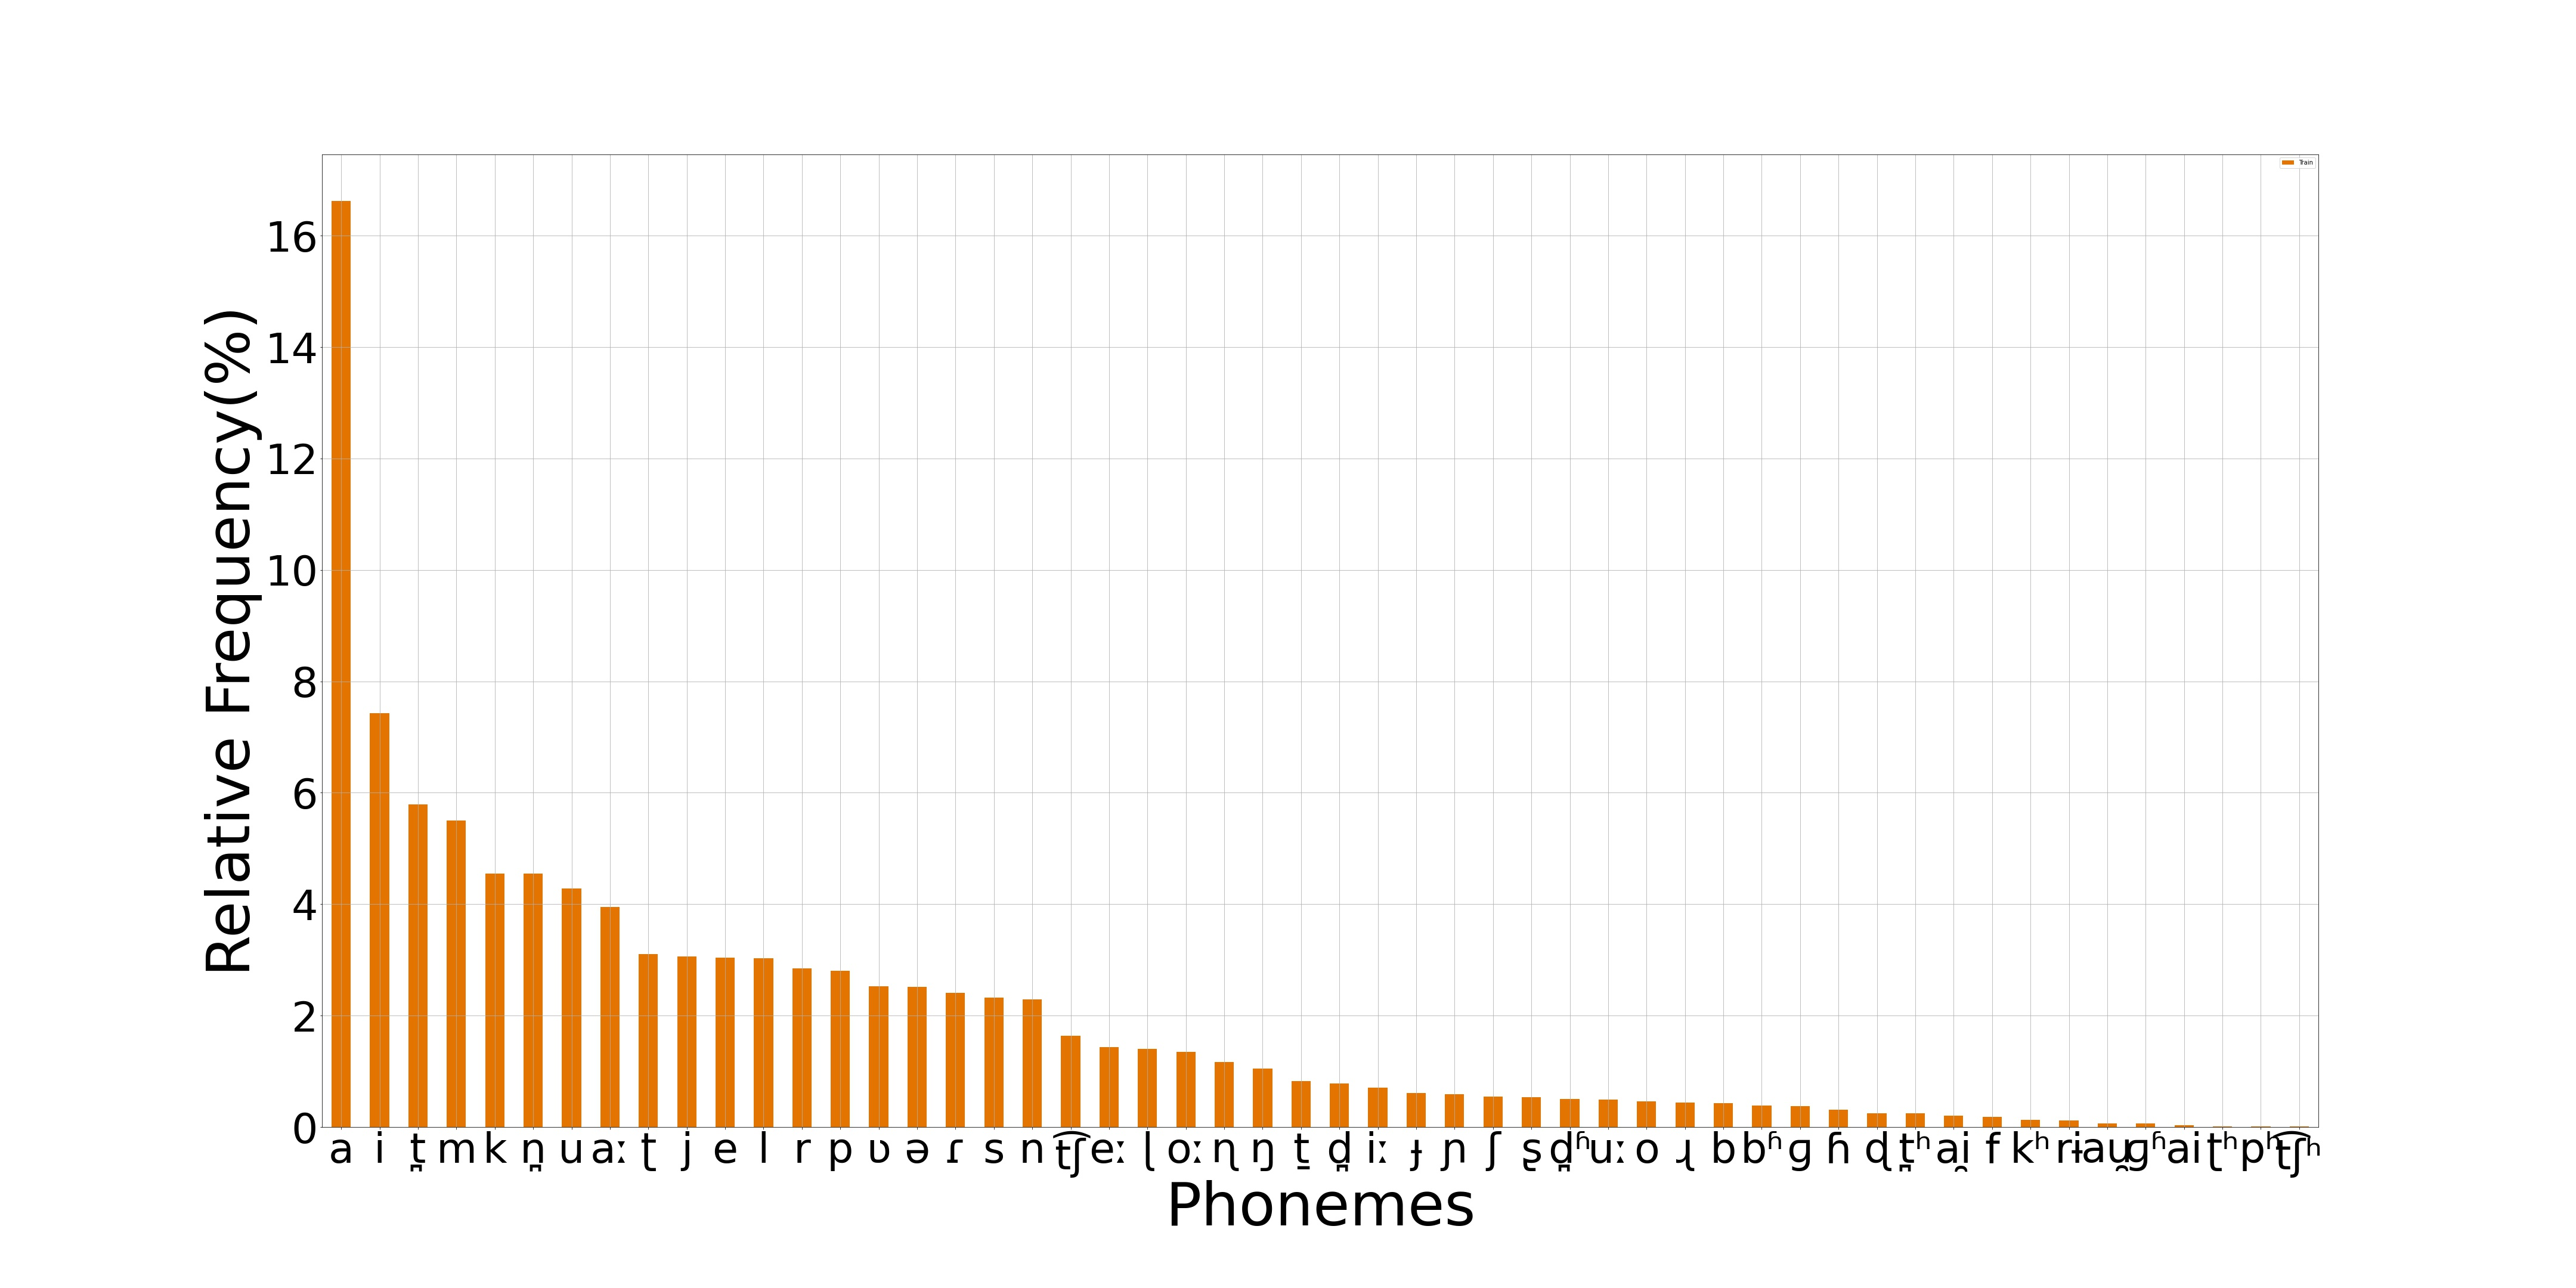
\includegraphics[width=\linewidth]{goldrichness.jpg}
    \caption{Phoneme diversity  analysis in gold standard lexicon}
    \label{goldrichness}
\end{figure}

A phoneme diversity analysis of the gold standard lexicon was performed and plotted in Fig. \ref{goldrichness}. The relative frequency of phonemes in gold standard lexicon follows the same pattern as previously reported values of phoneme diversity in Malayalam speech corpora \cite{smcspeech}.


\subsection{SYLLABIFICATION}

The syllabification results of Mlphon is evaluated on the gold standard reference. Even though the syllabification rules are deterministic there has been few deletion errors as illustrated in the Table \ref{goldsyl} and analysed in detail in section \ref{errorsyl}.

\begin{table}[h]
	\begin{center}
		\begin{minipage}{\textwidth}
			\caption{Comparing the syllabification provided by Mlphon with gold standard \\reference.}
			\label{goldsyl}

\begin{tabular}{lllc}
\hline \hline
 Word             & Reference             & Mlphon                   & Error       \\ \hline
{\mal ഈ} & {\mal ഈ.} &  {\mal ഈ.} & {-} \\
{\mal ഉന്നത} & {\mal ഉ.ന്ന.ത.} &  {\mal ഉ.ന്ന.ത.}& {- } \\
{\mal എന്ന}  & {\mal എ.ന്ന.}   &  {\mal എ.ന്ന.}  & {- } \\
{\mal  ഒരു}        & {\mal  ഒ.രു.}                      & {\mal  ഒ.രു.}                         & -            \\
{\mal കഫേ}       & {\mal ക.ഫേ.}                       &{\mal ക.ഫേ.}                        & -            \\
{\mal തോമസ്}      &{\mal തോ.മ.സ്.}     &    {\mal തോ.മ.സ്.}           & -  \\
{\mal നമ്പർ}      & {\mal ന.മ്പർ.}        &  {\mal ന.മ്പർ.}         & - \\
{\mal ഫലം}       & {\mal ഫ.ലം.}                     & {\mal ഫ.ലം.}                          & -            \\
{\mal ഫോട്ടോ}     &{\mal ഫോ.ട്ടോ.}                &{\mal ഫോ.ട്ടോ.}                         & -            \\
% 			10 {\mal മുന്നറിയിപ്പ്} & {\ipa m u \textbf{n n} a r i j i p p ə} & m u {\ipa n̪ n̪} a r i j i p p ə} & Substitution \\

{\mal സിഐഡി} & {\mal സി.ഐ.ഡി. }&  {\mal } & {Deletion} \\ \hline
\end{tabular}
		\end{minipage}
	\end{center}
\end{table}

\subsubsection{Syllabification Accuracy}

Accuracy is defined as a ratio between the correctly classified samples to the total number of samples. Precision  represents the proportion of positive samples that were correctly classified to the total number of positive predicted samples. Recall  of a classifier represents the positive correctly classified samples to the total number of positive samples. The harmonic mean of precision and recall is the F1 score \cite{tharwat2020classification}. The evaluation metrics averaged over all syllables and represented as percentage has the values as listed here.
% \begin{equation}
% \label{accuracy}
% Accuracy = \frac{ (True\ Positives + True\ Negatives) }{Total\ Samples}
% \end{equation}
%  as indicated in (\ref{pre}).
% \begin{equation}
% \label{pre}
% Precision = \frac{ True\ Positives }{(True\ Positives + False\ Positives)}
% \end{equation}

% \begin{equation}
% \label{recall}
% Recall = \frac{ True\ Positives }{(True\ Positives + False\ Negatives)}
% \end{equation} \cite{tharwat2020classification} as indicated in (\ref{f1}).
% \begin{equation}
% \label{f1}
% F1\ Score = \frac{(2 * Precision * Recall)} {(Precision + Recall)}
% \end{equation}



\begin{lstlisting}
	Accuracy	: 99%
	Precision	: 99%
	Recall		: 99%
	F1 Score	: 99%
\end{lstlisting}

\subsubsection{Syllable Error Rate}

We measure the syllable error rate (SER) based on the number of insertions, deletions, and substitutions for every syllable present in the gold standard lexicon.
% The result is given below.

% \begin{equation}
% 	\label{SER}
% 	SER = \frac{(I+D+S) × 100}{(N)}
% \end{equation}

\begin{lstlisting}
	Total Words: 1000
	Total Syllables:  2891
	Syllables deleted: 18
	Syllables Inserted: 0
	Syllables Substituted: 0
	Syllables Error Rate: 0.62%
\end{lstlisting}


\subsubsection{Error Analysis}
\label{errorsyl}

Among the words in gold standard lexicon, all syllabification errors were concentrated in words that are English abbreviations directly transliterated to Malayalam without any delimiters in between. Such words have violated the script grammar of Malayalam with vowels in word medial positions. Some Arabic loan words are among the other valid words that defy script grammar and cannot be syllabified by Mlphon.

\begin{figure}[h]
    \centering
    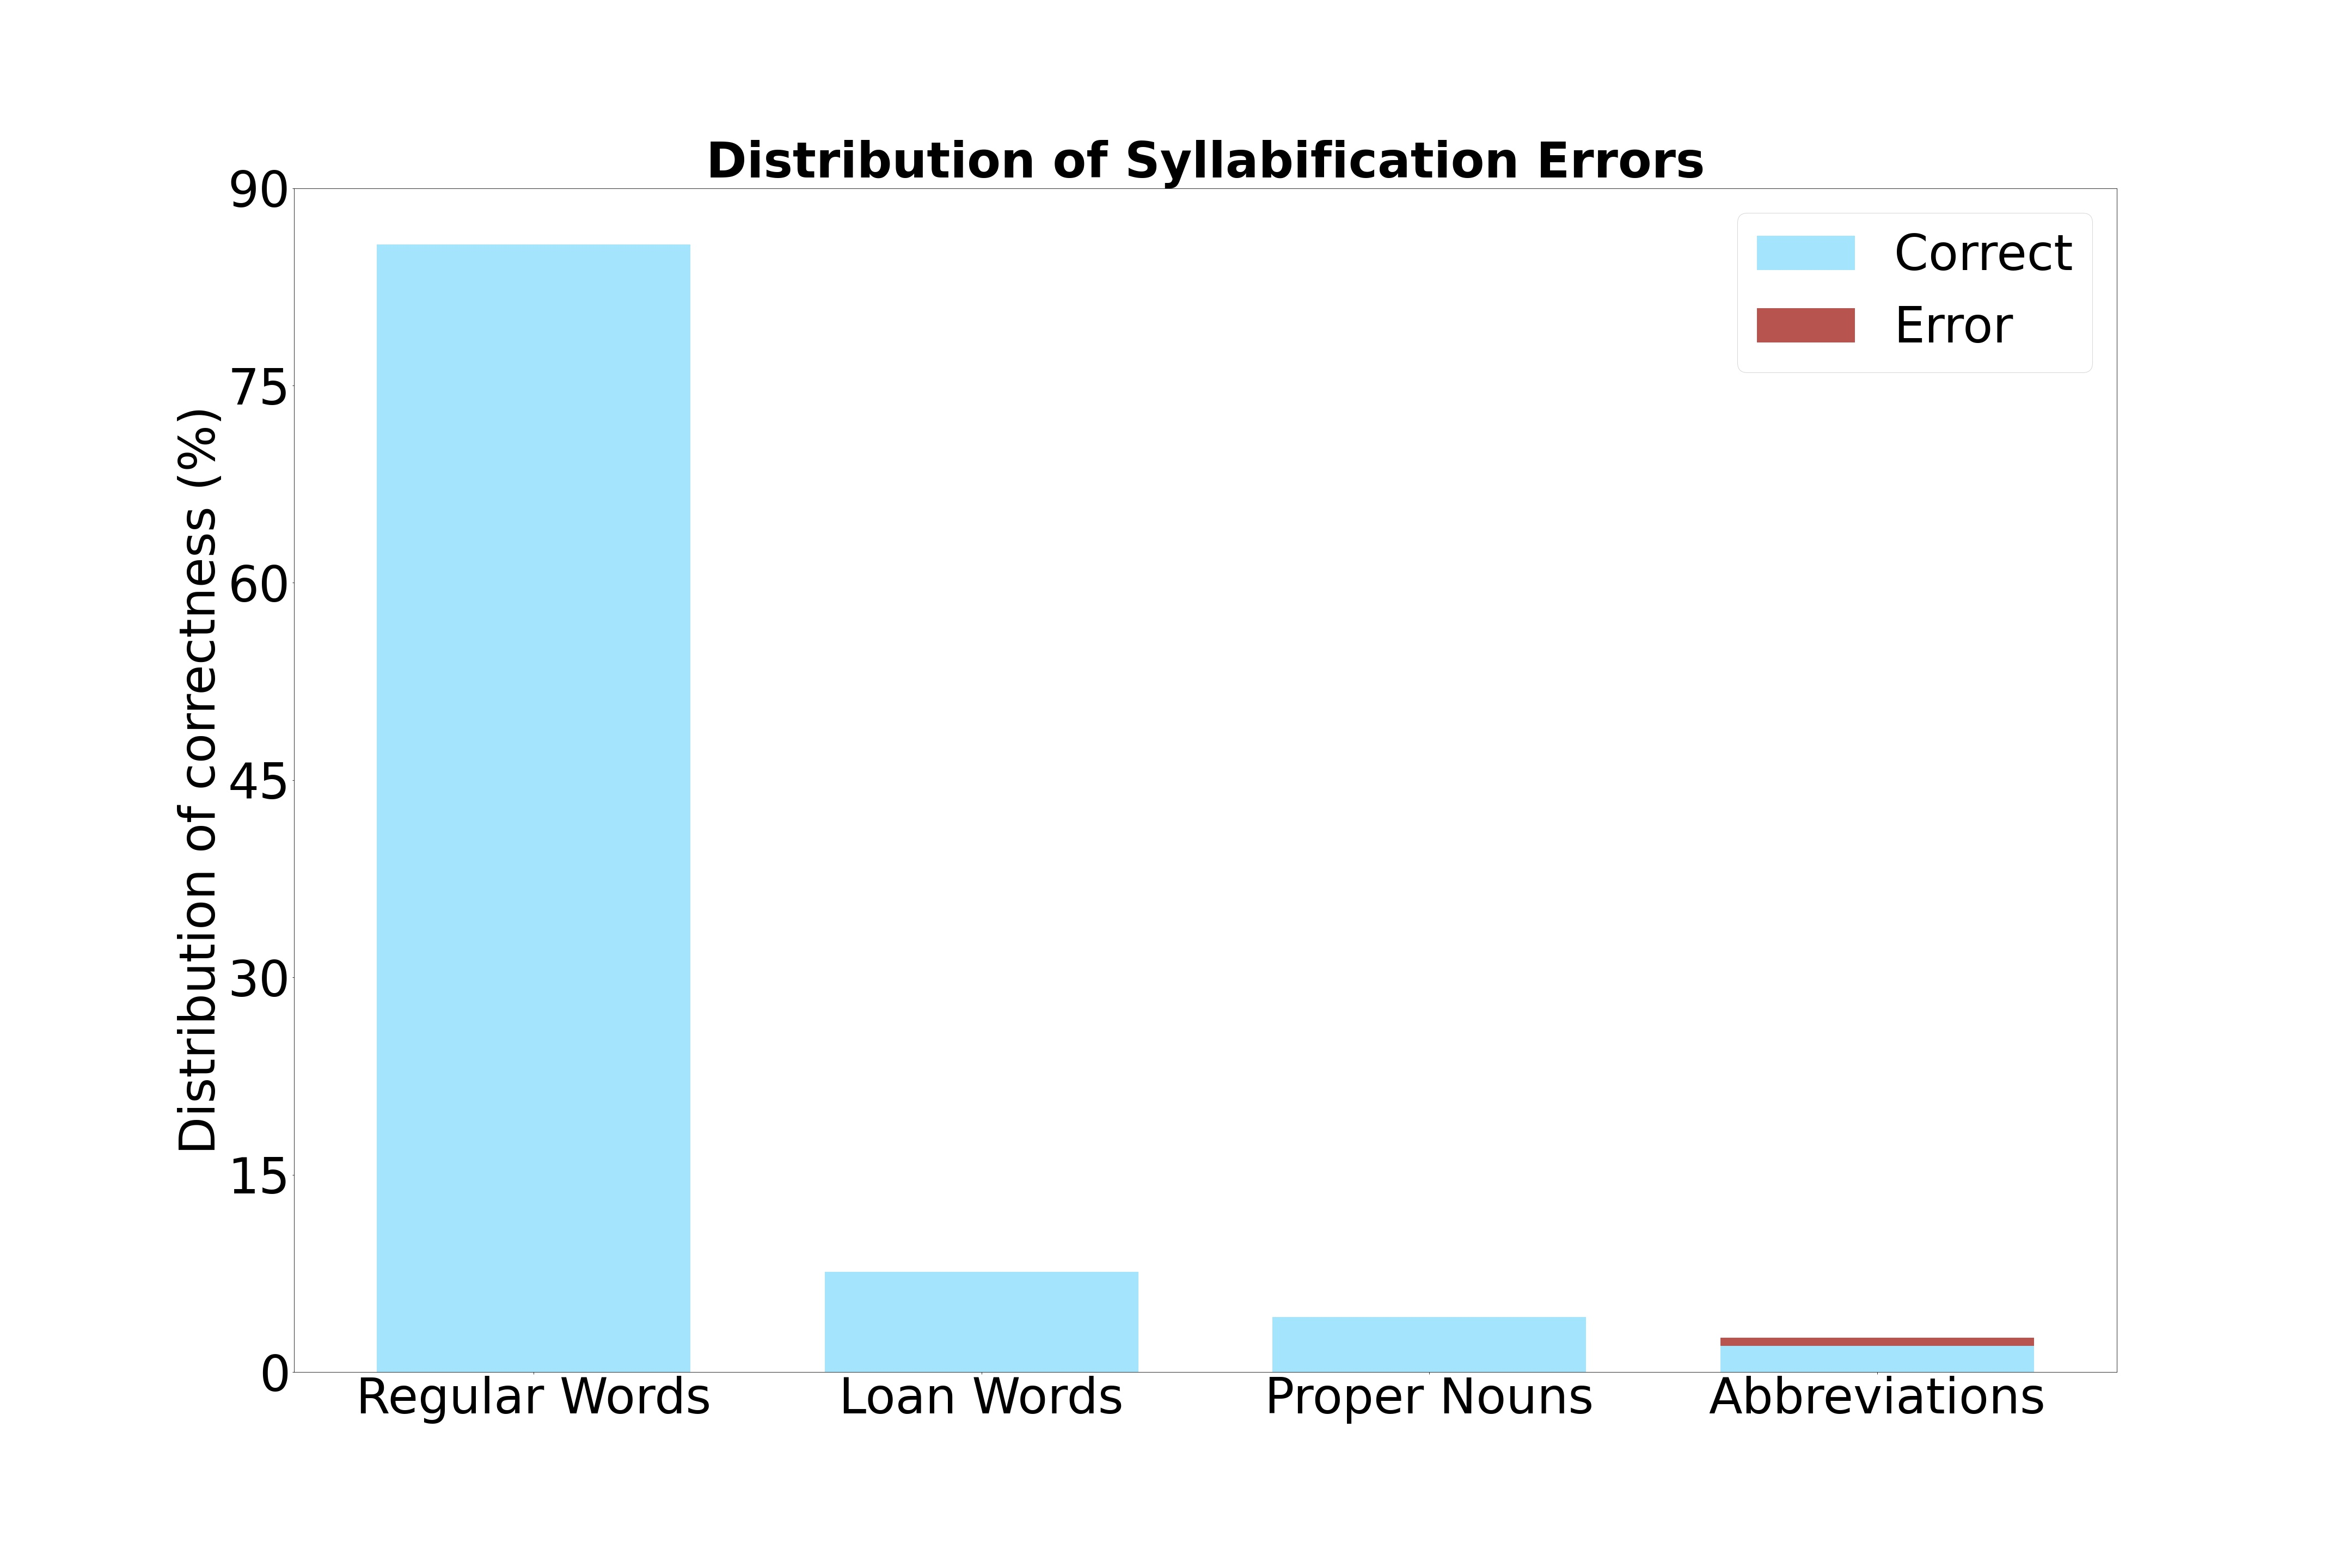
\includegraphics[width=0.9\linewidth]{syllable-error.jpg}
    \caption{Distribution of syllabification errors in different word types in gold standard lexicon}
    \label{syllable-error}
\end{figure}


When the word level syllabification errors were examined, 23\% of the abbreviations were incorrectly syllabified. This makes up about 0.6\% of  words in the entire gold standard lexicon. It is illustrated in Fig. \ref{syllable-error}.


\subsection{GRAPHEME TO PHONEME CONVERSION}

% As per the observations in 

% Word medial vowel graphemes which are considered to be invalid  by Mlphon, leads to deletion of that word without syllabification. However these errors could be corrected automatically by splitting the  words at positions of word medial vowels and passing as tokens to Mlphon. The following analysis on g2p conversion has been done after performing this correction.


The grapheme to phoneme conversion of Mlphon is evaluated, comparing its output with gold standard phoneme transcriptions. Evaluation involves phoneme level alignment of the transcription provided by Mlphon with that of the gold standard lexicon and counting the number of insertions, deletions and substitutions. We use the toolkit kaldialign\footnote{Kaldialign library \url{https://pypi.org/project/kaldialign/}} to perform the same. A sample of gold standard transcriptions with the phoneme sequence output provided by Mlphon is shown in Table \ref{gold}. 
% As discussed in section \ref{syllabletagger}, Mlphon checks for validity of character sequences. If there are vowel graphemes at middle of words, it is flagged as a lingustically invalid sequence and not parsed by FST. It is a common paractice in everyday news articles to have English acronyms transliterated to Malayalam without any delimiters (periods or spaces) in between. It effectively acts as a single word which has vowel graphemes at word middle positions. Such acronyms which are not transcribed by Mlphon, leads to deletion errors. In order to transcribe those acronyms, they are split at the positions of word medial vowels and are passed as tokens to Mlphon library. This is how the eleventh entry {\mal സിഐഡി} (C.I.D), with the vowel {\mal ഐ} in word medial position is correctly transcribed in the Table \ref{gold}.
\begin{table}[h]
	\begin{center}
		\begin{minipage}{\textwidth}
			\caption{Comparing the g2p transcription provided by  Mlphon with gold \\ standard reference.}
			\label{gold}
			\begin{tabular}{@{}p{1.7cm}p{1.5cm}p{1.5cm}p{1.5cm}@{}}
				\hline\hline
			 Word             & Reference             & Mlphon                   & Error        \\
				\hline
				{\mal ഈ}         & {\ipa iː}                               & {\ipa iː}                               & -            \\
				 {\mal ഉന്നത}      & {\ipa u n n a t̪ a}                      & {\ipa u n n a t̪ a}                      & -            \\
			 {\mal  എന്ന}       & {\ipa e n̪ n̪ a }                         & {\ipa e n̪ n̪ a}                          & -            \\
			 {\mal  ഒരു}        & {\ipa o ɾ u }                           & {\ipa o ɾ u}                            & -            \\
			 {\mal കഫേ}       & {\ipa k a f eː}                         & {\ipa k a f eː}                         & -            \\
			{\mal തോമസ്}      & {\ipa t̪ oː m a s}    &            {\ipa t̪ oː m a s} \textbf{{\ipa  ə}}            & Insertion    \\
			 {\mal നമ്പർ}      & {\ipa \textbf{n} a m p a r}            & \textbf{{\ipa n̪  }} {\ipa  a m p a r}             & Substitution \\
			 {\mal ഫലം}       & {\ipa  pʰ a l a m}                      & {\ipa pʰ a l a m}                       & -            \\
			 {\mal ഫോട്ടോ}     & {\ipa f oː ʈ ʈ oː}                      & {\ipa f oː ʈ ʈ oː}                      & -            \\
% 			10 {\mal മുന്നറിയിപ്പ്} & {\ipa m u \textbf{n n} a r i j i p p ə} & m u {\ipa n̪ n̪} a r i j i p p ə} & Substitution \\
			  {\mal സിഐഡി}     & {\ipa s i ai̯ ɖ i }                      & {\ipa s i ai̯ ɖ i }                      & -            \\
				\hline
			\end{tabular}
		\end{minipage}
	\end{center}
\end{table}


\subsubsection{Accuracy of g2p conversion }

Comparing the true phonemes in gold standard lexicons to the transcription provided by Mlphon, we present the phoneme transcription accuracy in the form of a confusion matrix in Fig. \ref{confusionmatrix}. For all phonemes other than those listed in Table \ref{precision}, the accuracy, precision, recall, and F1 scores were computed to be 100\%.
\vspace{0.2cm}

\begin{table}[h]
	\begin{center}
% 		\begin{minipage}{190pt}
			\caption{Precision, Recall and F1 Scores of phoneme transcription by Mlphon. For all other phonemes, these metrics are evaluated to be 100\%.}
			\label{precision}
			\begin{tabular}{@{}cccc@{}}
				\hline\hline
				Phoneme  & Precision (\%) & Recall (\%) & F1 Score (\%) \\
				\hline
				{\ipa n} & 100      & 84   &  91     \\
				{\ipa n̪} &92     & 100   & 96   \\
				{\ipa ə} & 93     & 100   &  97     \\

				\hline
			\end{tabular}
% 		\end{minipage}
	\end{center}
\end{table}


Except for the {\mal ന} disambiguation rules, all contextual rule sets operate flawlessly without a single error when evaluated on gold standard lexicon. The unintentional insertion of \textit{samvruthokaram} into non native proper names and abbreviations transliterated from English was the cause of all the insertion errors.  Insertion is mapped to the empty symbol `\#' in the gold standard transcription.  The top row of the Fig.\ref{confusionmatrix} shows insertion of `{\ipa ə}'. 
Since the mostly ambiguous  grapheme {\mal ഫ} was g2p mapped with 100\% accuracy on the gold standard lexicon, we increased the evaluation space to include 100k common Malayalam words.
According to the confusion matrix in Fig. \ref{faconfusion}, the transcription accuracy of {\mal ഫ} dropped to 99\% in the expanded evaluation set. 

% There are some ambiguities in resolving alveolar nasal from dental nasal as listed in rows 7 of Table \ref{gold} and it can be clearly seen in the confusion matrix too.However there has been no occurrence of wrong mapping of the {\mal ഫ} in the  gold standard lexicon.


The overall evaluation metrics averaged over all phonemes in the gold standard lexicon has the values in percentage as listed here.



\begin{lstlisting}
	Accuracy	: 99%
	Precision	: 98%
	Recall		: 98%
	F1 Score	: 98%
\end{lstlisting}


\begin{figure}[h]
	\centering
	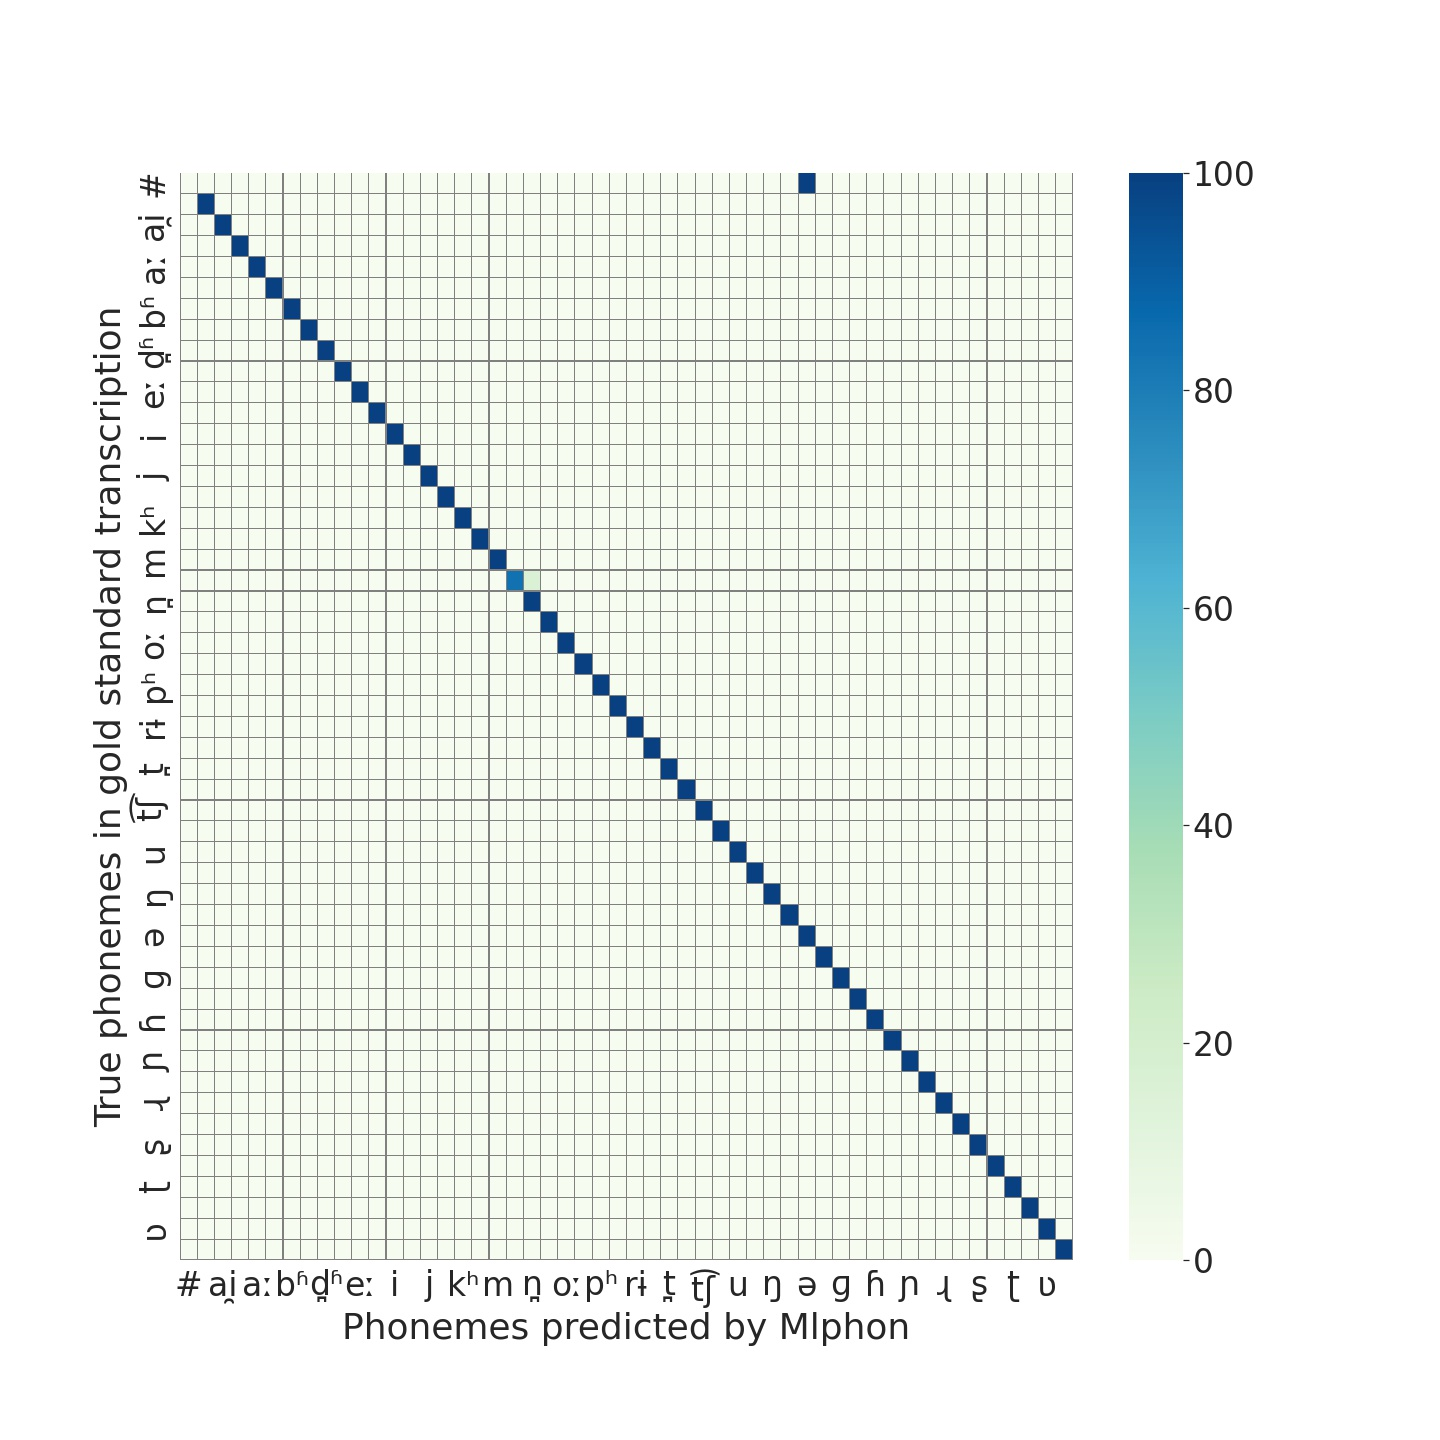
\includegraphics [width=\linewidth, height=10cm]{confusion.jpg}
	\caption{Confusion matrix comparing Mlphon transcription with gold standard transcription. The values are normalized and represented as percentage.}
	% \Description{Confusion matrix comparing Mlphon transcription with gold standard transcription}
	\label{confusionmatrix}
\end{figure}


\begin{figure}[!h]
	\centering
	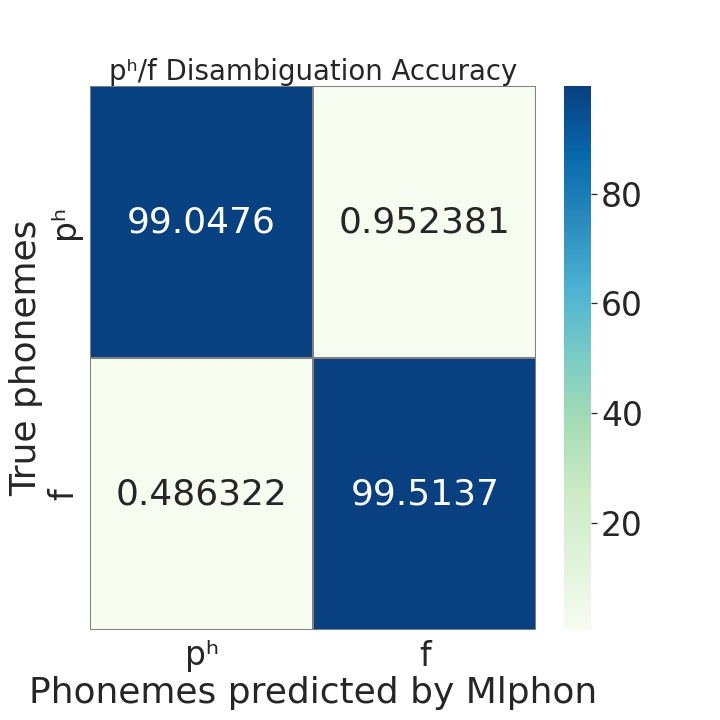
\includegraphics[width=0.6\linewidth]{fa.jpg}
	\caption{In an evaluation space of 100k tokens, we computed the accuracy of transcribing  {\mal ഫ}. The two possible pronunciations /{\ipa f}/ and /{\ipa pʰ}/ were accurately identified in more than 99\% of the cases as shown in this confusion matrix.}
 
 % Confusion matrix comparing transcription errors of  in a lexicon of 100k common words. The values are normalized and represented as percentage.}
	% \Description{Confusion matrix comparing transcription errors of {\mal ഫ} in a lexicon of 100k common words.}
	\label{faconfusion}
\end{figure}

\subsubsection{Phoneme Error Rate}

As an alternate metric to measure the phoneme transcription quality, we evaluate the phoneme error rate (PER). It is computed based on the number of insertions, deletions, and substitutions for every phoneme present in the gold standard lexicon.



% \begin{equation}
% 	\label{PER}
% 	PER = \frac{(I+D+S) × 100}{(N)}
% \end{equation}

\begin{lstlisting}
	Total Words: 1000
	Total Phonemes:  6755
	Phonemes deleted: 0
	Phonemes Inserted: 12
	Phonemes Substituted: 25
	Phoneme Error Rate = 0.55%
\end{lstlisting}


\begin{table*}[th]	
    \caption{A qualitative linguistic comparison between the lexicons produced by Mlphon and freely accessible automated tools}
    \label{lexiconcomparison}
    \begin{tabular}{@{}p{0.3cm}p{1cm}p{1.5cm}p{1.3cm}p{1.3cm}p{10cm}@{}}
    \hline \hline
  No. &  Word 							& Unified Parser 						& Espeak 						& 	Mlphon	& Remarks				  	\\
    \hline  
  1&  {\mal കല്പന}			  &	{\ipa k a \textbf{l} p a n a}				         &{\ipa k ɐ l b ə n ɐ}       &{\ipa k a l p a n a}	& The third phoneme produced by Unified Parser is different in rows 1 and 2, which should	  		\\
  2&  {\mal കൽപന}			  &	{\ipa k a \textbf{lw} p a n a}				         &{\ipa k ɐ l b ə n ɐ}       &{\ipa k a l p a n a} &  have been same as produced by Espeak and Mlphon 	\\ \hline

 3&   {\mal അവന്}	 			&{\ipa a w a n}				               &{\ipa ɐ v ə n ɨ}       &{\ipa	a ʋ a n ə} &  Espeak and Mlphon ensures word end vowel (\textit{Samvruthokaram}) is rightly inserted, corresponding to \textit{virama} at word ends. But Unified Parser does not handle this.\\ \hline
4&     {\mal നിനക്ക്}			  &	{\ipa n i n a k k}				         &{\ipa n i n ə kː ɨ}       &{\ipa	n̪ i n a k k ə} &	Only Mlphon disambiguates the dental ({\ipa	n̪} ) and alveolar nasal ({\ipa	n}) pronunciations of {\mal ന}. \\\hline
5&    {\mal കറന്റ്} 		& {\ipa k a rx a n rx}		& {\ipa k ɐ r ə n d ɨ}&  {\ipa k a r a n ṯ ə} & Unified Parser fails to contextually change the pronunciation of {\mal റ}, while Espeak and Mlphon handles this correctly\\
%   6&  {\mal നിനക്ക്}			  &	{\ipa n i n a k k}				         &{\ipa n i n ə kː ɨ}       &{\ipa	n̪ i n a k k ə}	\\
\hline
\end{tabular}
\end{table*}

\subsubsection{Error Analysis}

We performed a detailed analysis of g2p errors on different types of words in the gold standard lexicon. 1.4\% of regular words and 1.3\% of loan words had substitution errors. About 23\% of proper nouns and 15\% of abbreviations had insertion errors due to unintended \textit{samvruthokaram} at word ends. All the erroneous words account for 2.6\% of the total words in the gold standard lexicon. It is  illustrated in Fig. \ref{g2p-error}.

\begin{figure}[h]
    \centering
    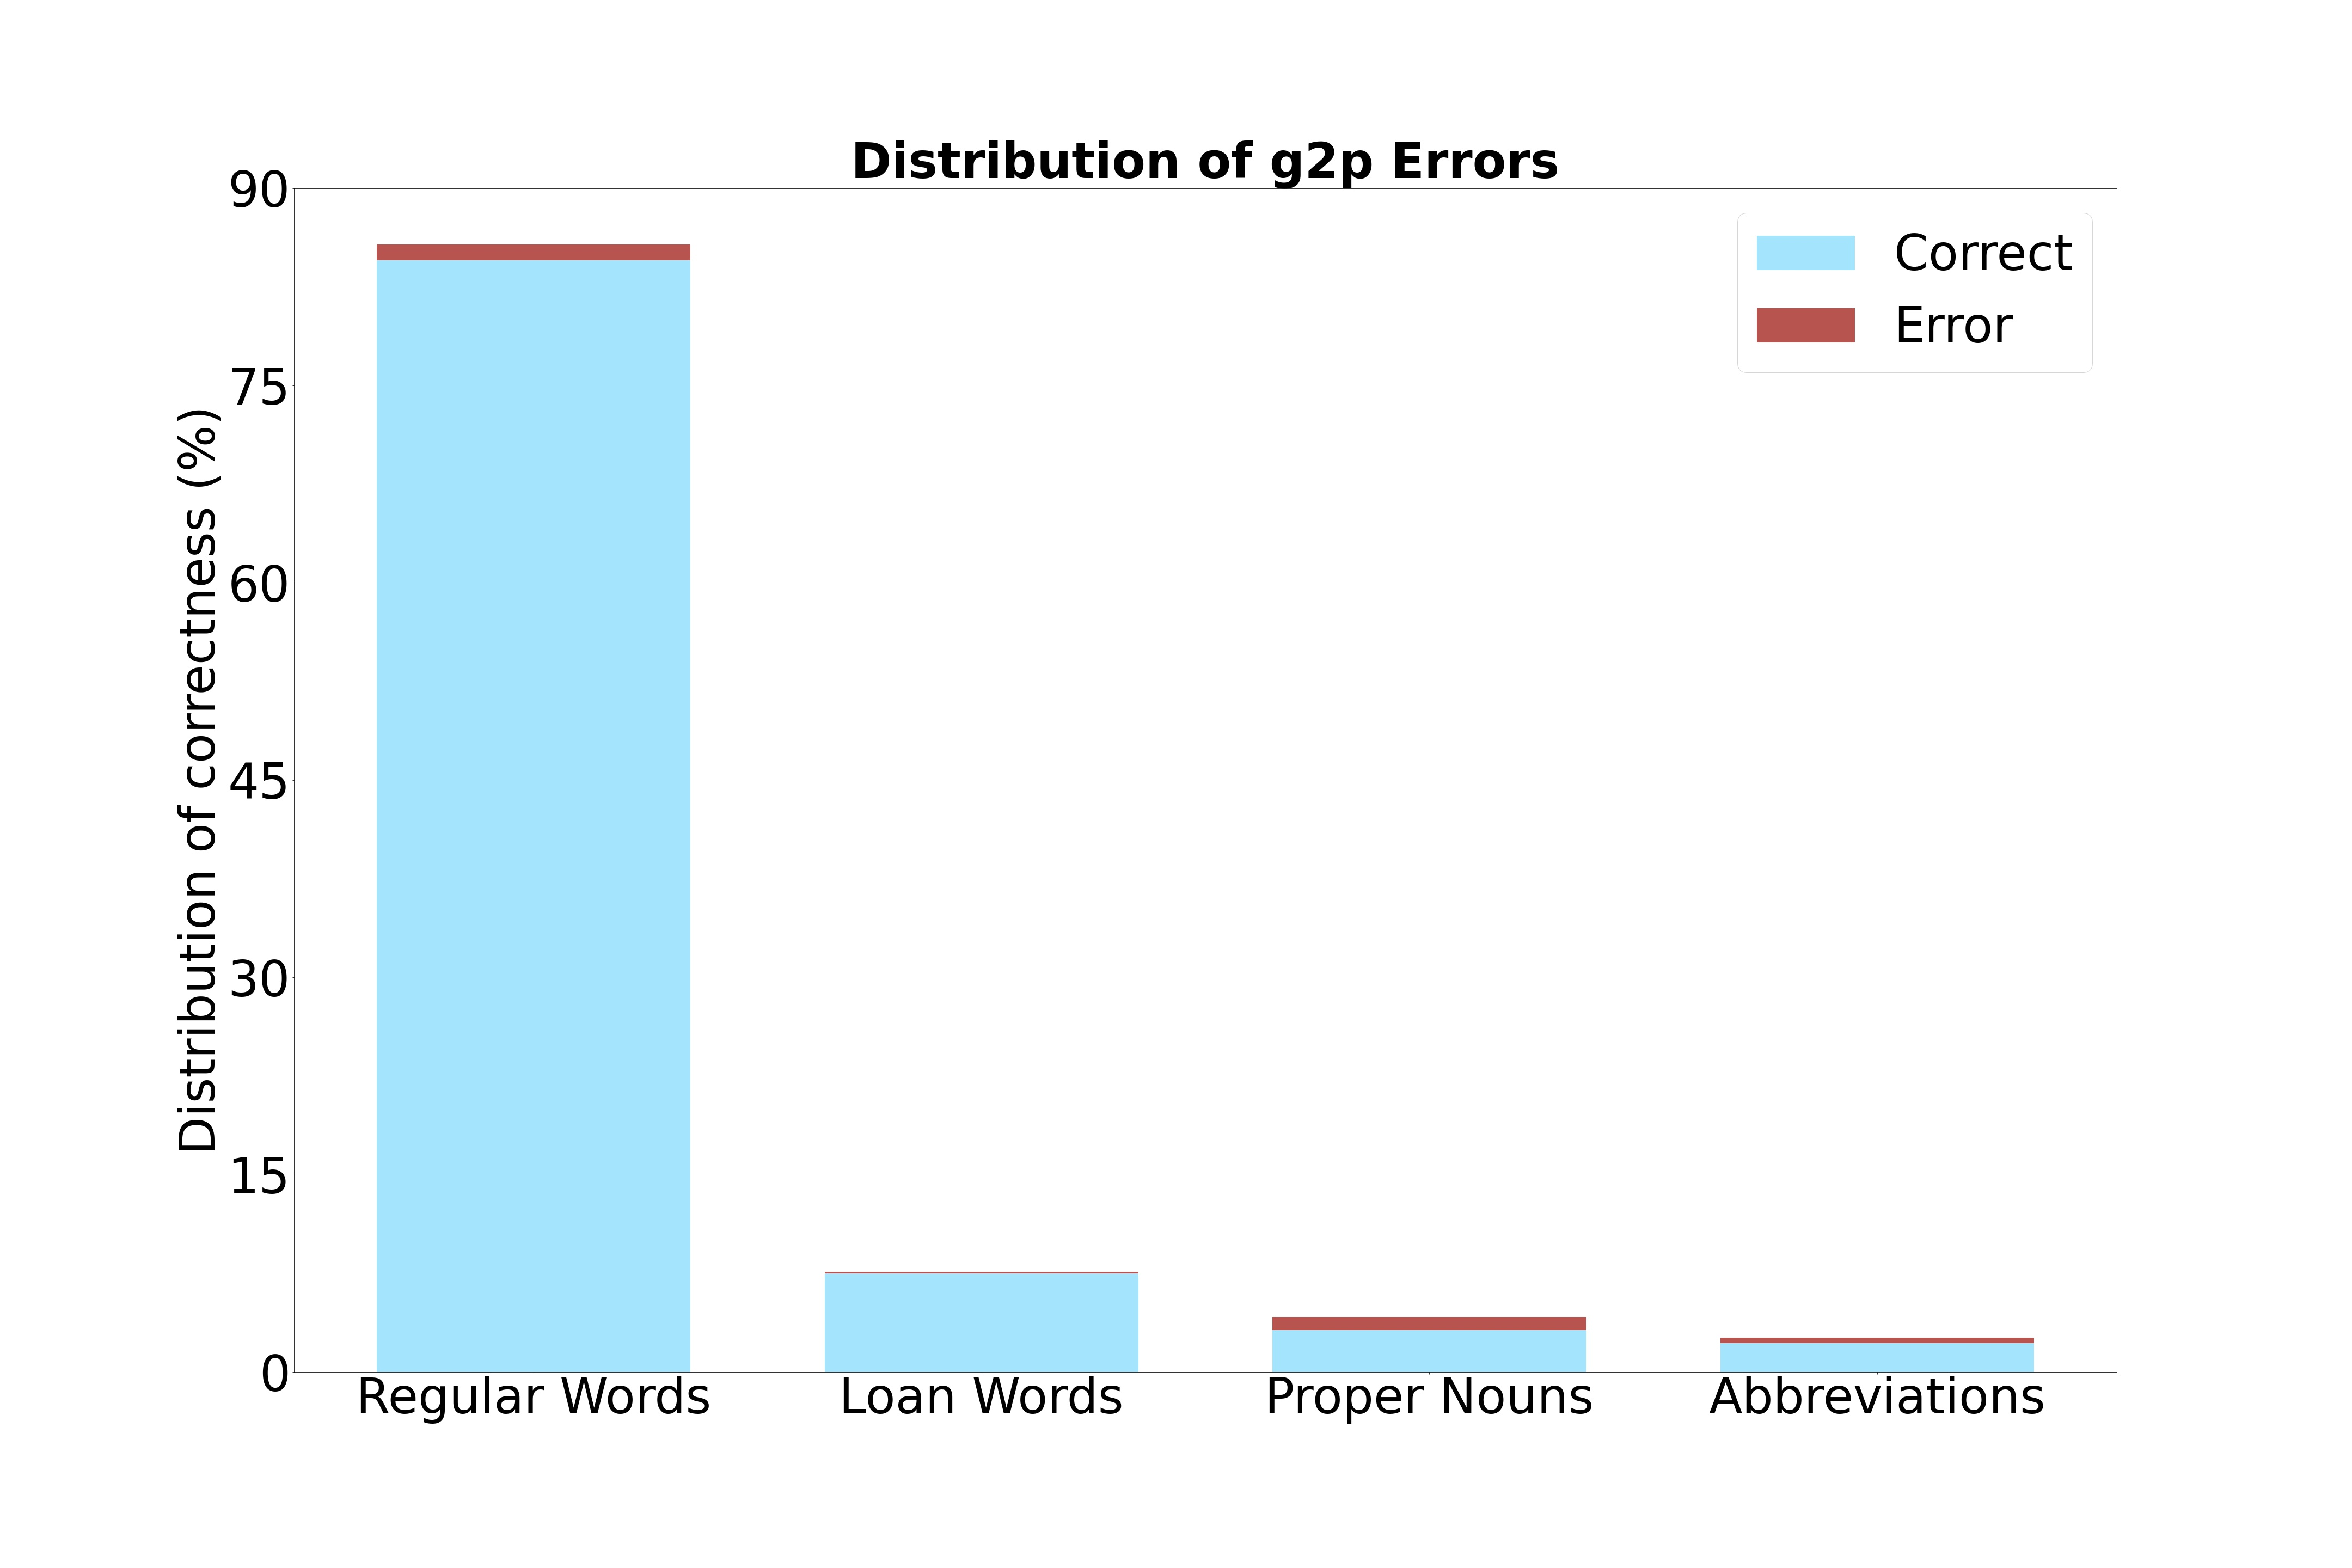
\includegraphics[width=\linewidth]{g2p-error.jpg}
    \caption{Distribution of g2p errors in different word types in gold standard lexicon.}
    \label{g2p-error}
\end{figure}



% All the contextual rule sets work perfectly without errors except the disambiguation rules for {\mal ന}. All the insertion errors are due to unintended insertion of \textit{Samvruthokaram} in non-native proper names. Since {\mal ഫ} is transcribed in the gold standard lexicon with 100\% accuracy, we expanded the evaluation space to 100k common words in Malayalam. It gave an accuracy above 99\% for transcription of {\mal ഫ} as shown in the confusion matrix in Fig. \ref{faconfusion}.



The correction of substitution and insertion errors involve morphologically analysing the words, which is currently beyond the scope of this work. Even with these limitations, the PER on the gold standard lexicon that covers about 26\% of words from 167 million tokens is only 0.55\% 
% \section{DISCUSSION WITH OTHER TOOLS ON G2P TASK}



\section{EVALUATIONS AND COMPARISON WITH OTHER TOOLS}
\label{asr}

The development of a pronunciation lexicon for use in speech tasks like ASR is one of the crucial applications of a g2p conversion tool. Of all the tools previously reported in literature, only Unified Parser and Espeak  are freely available to create Malayalam pronunciation lexicons on demand, with delimiters between phonemes. We build lexicons with Unified Parser and Espeak in order to compare and contrast Mlphon's performance with those tools. 

All of these tools use different phoneme alphabets. Additionally, the g2p mapping criteria vary. Unified Parser and Mlphon both aim to turn graphemes into phonemes. Espeak aims to create allophones of phonemes, which means that a particular phoneme may be represented by multiple phonetic symbols in Espeak, depending on where it appears in a word.  In the lexicons created for our ASR experiments, Mlphon has a set of 56 phonemes, whereas Unified Parser and Espeak have 61 and 62 phonemes, respectively. Unified Parser has a higher phoneme count because it differentiates  phonemes if they come from different graphemes. In contrast to the other two tools, Espeak uses distinct phonetic alphabets for allophonic variations, giving it a higher phoneme count.  Consequently, it is impossible to compare the output produced by these tools in a straightforward, direct, and automated manner.

Sample entries from the pronunciation lexicons created using these tools, are presented in Table \ref{lexiconcomparison}. On analysing these lexicons, following observations can be made:

\begin{enumerate}
    \item Unified Parser ignores all other contextual rules discussed in section \ref{arch}, except inherent vowel deletion in the context of \textit{virama} and other signs.
    % \item The third phoneme (in boldface) produced by Unified Parser is different in rows 1 and 2, which should be pronounced the same, even though they have different orthographic representations. However both Espeak and Mlphon handles this situation rightly.
    \item Espeak implements most of the contextual rules discussed in section \ref{arch}, except reph sign, dental nasal and labial plosive disambiguation.
    \item Espeak additionally considers allophonic variations due to co-articulation effects. Mlphon does not consider this because this is not a phonemic change.
\end{enumerate}

The carefully crafted pronunciation rules in Mlphon has close to perfect g2p mappings. It makes Mlphon suitable for the creation pronunciation lexicons and for linguistic learning purposes. The unattended contextual rules make Unified Parser less suitable for such tasks. Espeak is suitable to identify allophonic variations. The impact of these lexicons on ASR task is experimentally analysed and presented below.

% The pronunciation lexicon contains words and their pronunciation as a sequence of phonemes.

% To create a pronunciation lexicon for training the ASR, we have chosen the 100k common words lexicon described in Section \ref{pronunciationdictionary}. It is then expanded with the words from the training audio transcripts and words with atleast four occurrences from the language model training corpus. 


 %We employ the pipeline approach for ASR architecture where the the acoustic model, the pronunciation lexicon and the language model are different components that work together as a system. 

%
% In the pipeline approach, transcribed audio data requirement is much lesser than that in an end-to-end architecture of ASR for the same level of recognition accuracy \cite{Rosenberg2017, drexler2020improving}. This factor is very crucial considering the low resource nature of Malayalam.

%Many end-to-end systems are prohibitive to be used in embedded system applications due to their high computational and memory requirements. Kaldi TDNN chain model has proven to be an optimal solution with minimum memory and computational requirements for use in embedded applications without much compromising the recognition accuracy \cite{georgescu2021performance}.  To ensure good performance on embedded applications as well, we use Kaldi toolkit \cite{povey2011kaldi} for our experiments on ASR, with pronunciation lexicons created using Mlphon .

%(ii) Phonemizer\footnote{Python package phonemizer \url{https://pypi.org/project/phonemizer/}}  with Espeak backend and (iii) Unified Parser\footnote{Unified Parser source code \url{https://www.iitm.ac.in/donlab/tts/unified.php}}  \cite{baby2016unified}.

%\subsubsection{Speech Datasets}

%We have employed publicly available Malayalam speech corpora present in different multilingual datasets, namely,

% The speech datasets used are OpenSLR\footnote{OpenSLR Malayalam speech corpus \url{http://openslr.org/resources/63/}} \cite{he-etal-2020-open}, Indic TTS \cite{baby2016resources} and Festvox IIITH database\footnote{Festvox IIITH Malayalam speech corpus \url{http://www.festvox.org/databases/iiit_voices/}} \cite{prahallad2012iiit}. The entire Indic TTS speech database is used for training, Festvox IIITH speech database is set aside for testing, Open SLR corpus is split into two parts, one for training and the other for testing.  We have strictly ensured there is no overlap of speakers in training and test datasets.



%\begin{table}
%	\caption{Training Speech corpora}
%	\label{trainingcorpus}
%	\begin{tabular}{cccc}
%		Corpus           & Duration   & Utterances & Speakers \\
%		& (HH:MM:SS) &            &          \\
%		\toprule
%		Open SLR (train) & 4:47:47    & 3446       & 37       \\
%		Indic TTS        & 13:58:20   & 8601       & 2        \\
%		\midrule
%		Total            & 18:46:07   & 12047      & 39       \\
%		\bottomrule
%	\end{tabular}
%\end{table}
%
%% \begin{table}
%% 	\caption{Test Speech corpora}
%% 	\label{testingcorpus}
%% 	\begin{tabular}{cccc}
%% 		Corpus & Duration  & Utterances & Speakers \\
%% 		 & (HH:MM:SS) & & \\
%% 		\toprule
%% 		Open SLR (test) &  00:48:02 & 680 & 5 \\
%% 		Festvox IIITH &  01:37:46 & 1000 & 1 \\
%% 		\bottomrule
%% 	\end{tabular}
%% \end{table}

%\subsubsection{Text Corpus for Language Modeling}

% Remaining 212k sentences are cleaned up to remove special characters, numerals and then they are unicode normalised to get the text corpus for language model training.
% The language model training corpus contain 212k unique sentences and 26k unique words.

% \subsubsection{Creation of Large Vocabulary Pronunciation Lexicon}
% \label{lexiconcreation}



% The pronunciation lexicon for ASR is created with this 121k words using Mlphon, which took 1 minute 45 seconds to complete 
% Mlphon is capable of automatic creation of pronunciation lexicon consuming considerably less amount of processing time. The reason for the time efficiency while using Mlphon can be attributed to the computationally fast determinised FSTs \cite{mohri-1997-finite}, upon which Mlphon is built.



\subsection*{ASR Experimental Setup}


Kaldi toolkit \cite{povey2011kaldi} is used for our experiments on ASR. We split the openly available transcribed Malayalam speech corpora from various sources \cite{prahallad2012iiit,baby2016resources, he-etal-2020-open}, into training and test datasets, ensuring non-overlapping speakers and speech transcripts as listed in Table \ref{speechdatasets}. This amounts to 19 hours of speech data for training and 2 hours of speech data for testing. Apart from the transcripts of speech which amount to 7924 unique sentences, we have utilized the curated collection of  text corpus published by SMC \cite{smctext} amounting to 205k unique sentences for language modeling. After combining these, we explicitly removed all sentences that are present in our test audio transcripts. Bigram language model is prepared on this language modeling corpus using SRILM toolkit \cite{stolcke2002srilm}. The  vocabulary of our ASR is 69k words and the lexicons are prepared using Unified Parser, Espeak and Mlphon.

\begin{table*}[]
  \caption{Details of Speech data sets used in our experiments. }
  \label{speechdatasets}
        \centering
  \begin{tabular}{clcclll}
    \hline \hline
    \textbf{Name}& \textbf{Corpus}                                      & \textbf{\#Speakers}      & \textbf{\#Utterances}    & \textbf{Duration} &  \textbf{Type}   & \textbf{Environment}   \\
        &                                   &      &     & (minutes) &    & \\
    \hline
    1&Indic TTS, IITM \cite{baby2016resources}- Train          &2                          & 8601                      &838                         & Read, Formal          &Studio \\
    2&Open SLR Malayalam \cite{he-etal-2020-open} - Train &37                         & 3346                      &287                      &  Read, Formal         &Studio \\ 
    T1&Open SLR Malayalam \cite{he-etal-2020-open} - Test  &7                          & 679                       & 48                       &  Read, Formal         &Studio \\ 
    T2&Festvox IIITH \cite{prahallad2012iiit} - Test            &1                          &1000                       & 98                        & Read, Formal          &Studio \\
    % T3&MSC \cite{smcspeech}   -Test                             & 75                        &1541                       & 98                       & Read, Conversational & Natural, Noisy \\

    \hline
    
    
  \end{tabular}

\end{table*}


The speech sampling rates of different sources are converted to a sampling frequency of 16 kHz prior to feature extraction.  As the acoustic features, we have used standard Mel frequency cepstral coefficients (MFCCs) with delta and double delta coefficients computed over a window (Hamming) size of 25 ms with an overlap of 10 ms for GMM-HMM monophone and triphone models. The acoustic modeling begins with flat start monophone model followed by context dependent triphone acoustic modeling. Then speaker independent linear discriminant analysis (LDA) to reduce the feature space dimensionality and maximum likelihood linear transform (MLLT) are performed. It is followed by triphone speaker adaptive training (SAT).
%The sampling rates of audio in OpenSLR and Indic TTS corpora are 48kHz and in the Festvox IIITH corpus it is 16kHz. The first two datasets were down sampled to 16kHz


Phone alignments from final triphone model are used for Kaldi chain acoustic modeling. It is implemented using time delay neural networks (TDNNs) \cite{peddinti2015time}. Acoustic features used in TDNN training are: (i) 40-dimensional high-resolution MFCCs extracted from frames of 25 ms length and 10 ms shift and (ii) 100-dimensional i-vectors \cite{saon2013speaker} computed from chunks of 150 consecutive frames. Three consecutive MFCC vectors and the i-vector corresponding to a chunk are concatenated, obtaining a 220-dimensional feature vector for a frame. Neural acoustic model is trained on a single NVIDIA Tesla T4 GPU. 

% I-vectors are a kind of feature containing speaker characteristic information and  they have a role in improving the system’s adaptation to the specific speech of a speaker \cite{georgescu2021performance}. We have used audio data augmentation by speed and volume perturbation before i-vector extraction  \cite{ko2015audio}. 

% IRST Language Modeling (IRSTLM) toolkit  \cite{federico2008irstlm} is used for building bigram word level language model, from the 212k sentences for language modeling. Pronunciation lexicons with word vocabulary size of 121k, generated with Mlphon is employed in our experiments.



\subsubsection*{Result Analysis }

All the ASR models use the same bigram language model, with different acoustic models and pronunciation lexicons. The performance of  ASR models are evaluated in terms of WER.  WER is computed based on the number of words inserted (I), deleted (D) and substituted (S) in the predicted speech transcript when compared to the ground truth transcript.

% \begin{equation}
% 	\label{wer}
% 	WER = \frac{(I+D+S) × 100}{(N)}
% \end{equation}

The OOV rates and dataset characteristics have a significant impact on the ASR results. It is also largely influenced by the domain of text used in language modeling. We evaluate our ASR models on two different test datasets namely, T1 (14\% OOV) and  T2 (1\% OOV) derived respectively from OpenSLR \cite{he-etal-2020-open} and Festvox IIITH \cite{prahallad2012iiit} corpora that contains 48 and 98 minutes each of speech data. The test data set with lower OOV rate performs better as expected. The resulting WER produced by the lexicons created using all tools under investigation are reported in Table \ref{result}. The best WERs on T1 and T2 are 34.6\% and 9.6\% respectively, and they are both given by Mlphon lexicon.

\begin{table}[h]
	\caption{Comparing WER (\%) obtained in Malayalam ASR experiments with lexicons created using the proposed tool, Mlphon, and other openly available tools.}
	\label{result}

	\begin{tabular}{@{}|l|ccc|ccc|@{}}
\hline \hline	
&  \multicolumn{3}{c}{{\textbf{T1 (14\% OOV)}}} &\multicolumn{3}{|c|}{{\textbf{T2  (1\% OOV)}}}                                                                                                                                                         \\
% 		\cmidrule(l){2-8}

\text{\textbf{Acoustic Models}} &  \rotatebox{90}{\textit{Unified Parser}}  & \rotatebox{90}{\textit{Espeak}}        & \rotatebox{90}{\textit{Mlphon}} & \rotatebox{90}{\textit{Unified Parser}} & \rotatebox{90}{\textit{Espeak}} & \rotatebox{90}{\textit{Mlphon}} \\
\hline
	Monophone   &60.9  & \textbf{58.4} & 58.7& 25.0&\textbf{20.9} &  21.8                                                               \\
	Triphone	&49.9 &48.3 &\textbf{47.4} &21.0  & 17.5 & \textbf{17.1 }\\
	Triphone (LDA) &43.8 & \textbf{41.2} & 43.7&  18.4&14.3   & \textbf{13.9}\\
	Triphone(SAT)	&43.6&41.2& \textbf{41.0}& 14.3&11.1 &\textbf{10.6} \\

TDNN & 35.7& 34.9&\textbf{34.6 }&10.7 & 9.7&\textbf{ 9.6}\\
\hline	\end{tabular}
\end{table}

% \begin{figure}

% 		\centering
% 		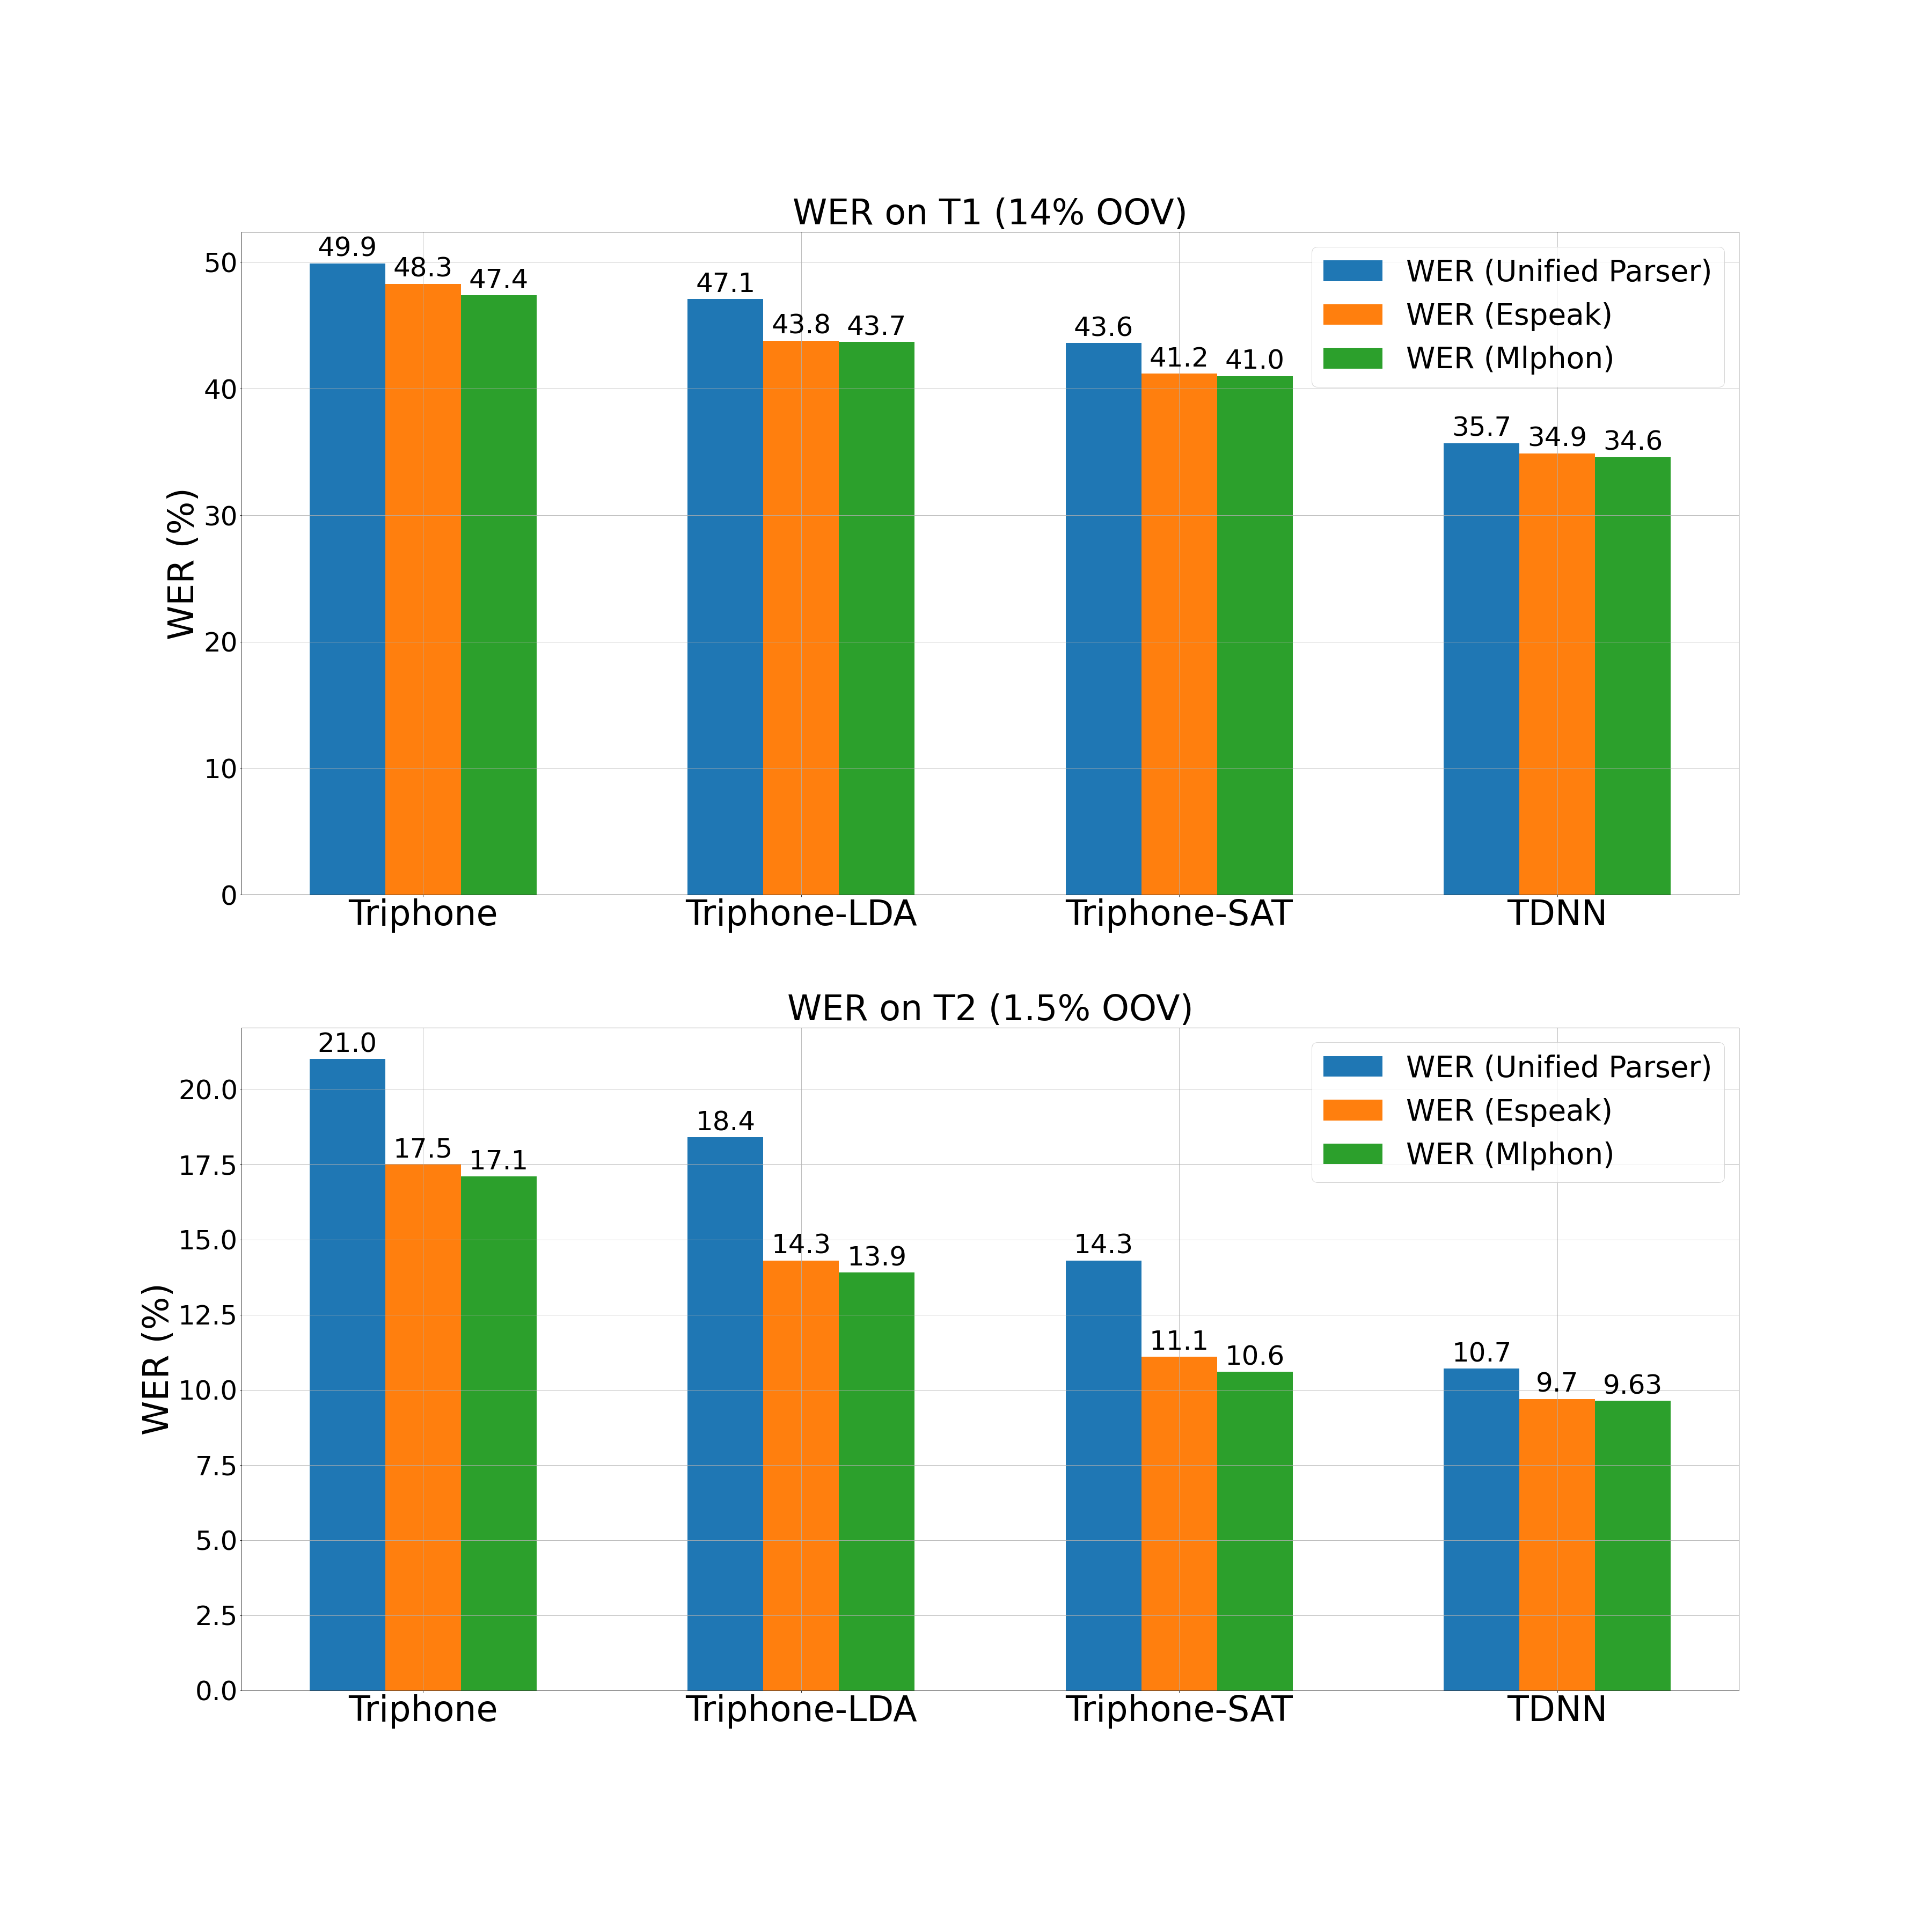
\includegraphics[width=\linewidth]{WER3.png}
% 	\caption{Plot showing WER obtained in Malayalam ASR experiments with different lexicons and acoustic models.}
% 			\label{wer3}
% %
% \end{figure}


 These results can be used to deduce some interesting insights about the impact of phoneme transcription quality on WER. It has been found that Mlphon lexicon performs the best with most of the acoustic models, closely followed by Espeak lexicon. The meticulously crafted pronunciation rules have an effect on this improved WER. The context-free monophone acoustic model works well with the Espeak lexicon. This might be as a result of the contextual co-articulation effects being already included in the Espeak lexicon. The Unified Parser Lexicon performs poorly in terms of WER because it ignores the majority of the contextual rules highlighted in section  \ref{arch}.


% Mlphon is designed as a computational linguistic tool that provides accurate phonemic transcription of graphemes. It does not take into account the allophonic variations. The transcription provided by Espeak is mostly phonetic in nature. Even though it does not dismabiguate alveolar and dental nasals (for the grapheme {\mal ന}) and labial plosive and labiodental fricative (for the grapheme {\mal ഫ}) as Mlphon does, it captures most of the contextual phoneme changes implemented in Mlphon and provides transcriptions considering co-articulation effects too. But Unified Parser misses most of the contextual information while making transcriptions.

% The monophone model,  works best with Espeak. T The missing disabiguation rules in Espeak are lingustically rare in the acoustic model training corpus, making the errors irrelevent to be reflected in acoustic modeling. The triphone model which uses phonetic context while acoustic modeling gives the best WER with Mlphon based lexicon. The TDNN chain model brings a significant improvement in the acoustic modeling with larger temporal contexts. This could have evened out the missing contextual information from the Unified Parser based lexicon, making it the best performer with TDNN chain model. With TDNN model, the performance of other lexicons closely follows the best one (See Fig. \ref{wer}).

This analysis is an indicator of the importance of precise g2p conversion required for speech tasks. Also as we demonstrate in the following section, Mlphon has the additional advantage of high word processing speed, while creating pronunciation lexicons.

Although there have been previously published works on ASR for continuous Malayalam speech \cite{lavanya2018,deekshitha,lekshmi2021}, each one was tested using private datasets described in respective papers. The lexicon creation process was not explicitly explained. Additionally, some of these works did not mention the sizes of the pronunciation lexicon and OOV rates, which have a significant impact on the WER. Nevertheless we present a comparison of these previously reported WERs with ours. It is observed that, on two different test datasets of OOV rates 14\% and 1\%, the proposed ASR with Mlphon lexicon provides similar or better WERs when compared with previously reported WERs as listed in Table \ref{asrcomparison}. 

\begin{table}[h]
	\caption{Comparison of WER from previously reported works on  Malayalam ASR. The ASR we built using the lexicon created with Mlphon performs at par with the previously reported works.}
	\label{asrcomparison}
	\begin{tabular}{lcc|c}
 \hline \hline
 \textbf{ASR Model} & \textbf{Lexicon size} & \textbf{OOV Rate (\%)}& \textbf{WER (\%)} \\
 \hline
 Deekshita et al.\cite{deekshitha} & 29k & 8 & 34.2 \\
 Lavanya et al. \cite{lavanya2018} & - & - & 34.4 \\
Lekshmi et al. \cite{lekshmi2021} & - & - & 10.0 \\
Proposed tool & 69k & 14& \textbf{34.6} \\
Proposed tool & 69k & 1& \textbf{9.6}\\

\hline	\end{tabular}
\end{table}


\begin{table*}[ht]
\centering
	\begin{center}
		\begin{minipage}{\textwidth}
			\caption{Pronunciation lexicons of different word categories.}
			\label{dictionaries}
			\begin{tabular}{@{}p{1.8cm}p{3cm}p{12cm}@{}}
				\hline
				\hline
				\textbf{Category} & \textbf{Number of lexical entries} & \textbf{Remarks}                                                                                                   \\
				\hline
				Common words      & 100000                             & Most commonly used 100k Malayalam word forms. They are arranged in the order of decreasing frequency. \\
				Verbs             & 3895                               & Malayalam verbs in the citation form arranged in alphabetic order                                                  \\
				Nouns             & 59763                              & Malayalam nouns arranged in alphabetic order                                                                       \\
				Proper nouns      & 6751                               & Common Malayalam person names, place names and brand names arranged in alphabetic order                            \\
				Foreign words     & 4350                               & Sanskrit and English borrowed words commonly used in Malayalam arranged in alphabetic order                        \\

				\hline
			\end{tabular}
		\end{minipage}
	\end{center}
\end{table*}

% Unified Parser lexicon which performed the best in terms of WER with TDNN chain model, requires very long computation time for its creation. Mlphon on the other hand has the advantage of being very compact and fast (See section \ref{pypi}, \ref{lexiconcreation}), requiring considerably less memory and computation time.



%The script specific contextual rules in Mlphon is a significant improvement when compared to language independent Unified Parser tool. In the baseline phonetic lexicon, the plosive phoneme /ṯ/ in geminated alveolar plosive {\mal റ്റ}, /ṯṯ/ and the alveolar conjunct {\mal ന്റ} /nṯa/, are wrongly mapped to the alveolar trill phoneme, /r/. This mismapping could have caused confusion during acoustic model training as well as decoding. Consonant \textit{chillu} graphemes in Malayalam have the phonetic characteristics same as that of the root consonant from which they are derived. While Mlphon maps them to the same phoneme as that of the root consonant, the baseline lexicon defines a separate phoneme for consonant \textit{chillu} graphemes. Additionally Mlphon maps the symbol {\mal ം} (anuswaram) to the labial nasal phoneme m, as per its pronunciation, while the baseline lexicon defines it as different phoneme. Unified parser does not take into account the word final schwa addition feature of Malayalam (samvruthokaram). Defining different phonetic representations to similar acoustic features could possibly introduce phoneme alignment errors during AM training. We attribute the performance improvement in terms of WER in Mlphon phonetic lexicon, to the more accurate phonetic transcription it provides.

\section{Creating Large Vocabulary Pronunciation Lexicons}
\label{pronunciationdictionary}

Apart from small pronunciation lexicons created manually or semi-automatically for some specific experiments as discussed in section \ref{motivation},  there is exists no openly available pronunciation lexicons for Malayalam. To bridge this gap we publish a large vocabulary pronunciation lexicon for Malayalam, automatically created using Mlphon. 


These lexicons consist of different categories of words as described in Table \ref{dictionaries}. The tokens in common words pronunciation lexicon are extracted from a general domain text corpus of 167 million types covering the fields of business, entertainment, sports, technology etc. as described in Indic NLP dataset \cite{kunchukuttan2020ai4bharat}. The rest of the categories are curated word lists from the Malayalam morphology analyser, Mlmorph \cite{thottingal-2019-finite}. Since Mlphon fails to syllabify and phoneme map abbreviations that contain word medial vowels, a work around script has been written to split such words at the position of vowels and obtain the right g2p results. 

These pronunciation lexicons are published in two separate formats; one with phoneme level transcription where pronunciation is described as a sequence of phonemes and the other with syllable level transcription where pronunciation is described as a sequence of syllables. The sequences are separated with a blank space in between. The lexicons are published in a two column, tab separated values (tsv) format. Multiple pronunciations of the same word are provided wherever applicable. 

Table \ref{lexiconsamples}  gives an excerpt from different categories of pronunciation lexicons. These lexicons are publicly available for download and usage under CC-BY-SA License.


% \vspace{0.2cm}
\begin{table}[!h]
	\begin{center}
		\begin{minipage}{\textwidth}
			\caption{An excerpt from pronunciation lexicons.}\label{lexiconsamples}
			\begin{tabular}{@{}p{1.2cm}p{1.5cm}p{2cm}p{2.2cm}@{}}
				\hline
				\hline
				Lexicon                      & Word              & Phonemised transcription          & Syllabified transcription  \\
				\hline
				\multirow{6}{*}{\rotatebox{60}{Common words}}   & {\mal ഒരു}         & {\ipa o ɾ uː}                     & {\ipa o ɾu}                \\
				                                & {\mal ഈ}          & {\ipa iː}                         & {\ipa iː}                  \\
				                                & {\mal എന്ന}        & {\ipa e n̪ n̪ a}                    & {\ipa e n̪n̪a}               \\
				                                & {\mal തന്നെ}       & {\ipa t̪ a n̪ n̪ e}                  & {\ipa t̪a n̪n̪e}              \\
				                                & {\mal പറഞ്ഞു}       & {\ipa p a r a ɲ ɲ u}              & {\ipa pa ra ɲɲu }          \\
				                                & {\mal എന്നാൽ}      & {\ipa e n n aː l}                 & {\ipa e nnaːl}             \\
				                                & {\mal എന്നാൽ}      & {\ipa e n̪ n̪ aː l}                 & {\ipa e n̪n̪aːl}             \\

				\hline
				\multirow{3}{*}{\rotatebox{60}{Verbs}}          & {\mal അകലുക}       & {\ipa a k a l u k aː}             & {\ipa a ka lu ka}          \\
				                                % & {\mal അംഗീകരിക്കുക} & {\ipa a m ɡ iː k a ɾ i k k u k a} & {\ipa am ɡiː ka ɾi kku ka} \\
				                                & {\mal അഞ്ചുക}       & {\ipa a ɲ t͡ʃ u k a}               & {\ipa a ɲt͡ʃu ka}           \\
				                                & {\mal അടക്കുക}      & {\ipa a ʈ a k k u k a   }         & {\ipa a ʈa kku ka}         \\

				\hline
				\multirow{4}{*}{\rotatebox{60}{Nouns}}          & {\mal അടക്ക്}       & {\ipa a ʈ a k k ə}                & {\ipa a ʈa kkə}            \\
				                                & {\mal അടങ്കൽ}      & {\ipa a ʈ a ŋ k a l}              & {\ipa a ʈa ŋkal}           \\
				                                & {\mal അടച്ചുതുറ}     & {\ipa a ʈ a t͡ʃ t͡ʃ u t̪ u r a}      & {\ipa a ʈa t͡ʃt͡ʃu t̪u ra}    \\
				                                & {\mal അടച്ചുവാറ്റി}  & {\ipa a ʈ a t͡ʃ t͡ʃ u ʋ aː ṯ ṯ i}   & {\ipa a ʈa t͡ʃt͡ʃu ʋaː ṯṯi}  \\
				\hline
				\multirow{4}{*}{\rotatebox{60}{Proper Nouns}}  & {\mal അക്ബർ}       & {\ipa a k b a r}                  & {\ipa a kbar}              \\
				                                & {\mal അക്ഷയ}       & {\ipa a k ʂ a j a}                & {\ipa a kʂa ja}            \\
				                                & {\mal അക്ഷര}       & {\ipa a k ʂ a ɾ a}                & {\ipa a kʂa ɾa}            \\
				                                & {\mal അഖില}       & {\ipa a kʰ i l a}                 & {\ipa a kʰi la}            \\
				                                				                                & {\mal അഖിലൻ}      & {\ipa a kʰ i l a n}                 & {\ipa a kʰi lan}            \\
				\hline
				\multirow{4}{*}{\rotatebox{60}{Loan words}} & {\mal അക്കാഡമി}    & {\ipa a k k aː ɖ a m i}           & {\ipa a kkaː ɖa mi}        \\
				                                & {\mal അക്കൗണ്ട്}     & {\ipa a k k au̯ ɳ ʈ ə}             & {\ipa a kkau̯ ɳʈə}          \\
				                                & {\mal അക്വേറിയം}   & {\ipa a k ʋ eː r i j a m}         & {\ipa a kʋeː ri jam}       \\
				                                & {\mal അങ്കിൾ}      & {\ipa a ŋ k i ɭ}                  & {\ipa a ŋkiɭ}              \\
				\hline
			\end{tabular}
		\end{minipage}
	\end{center}
\end{table}


\subsection{COMPARISON OF PROCESSING SPEED}

Word processing speed (WPS) is one indicator of a g2p algorithm's effectiveness \cite{mdpi2022ruleg2p}. The WPS  for the applications, Unified Parser \cite{baby2016unified}, Espeak\footnote{Using Phonemizer library \url{https://pypi.org/project/phonemizer/}} and the proposed tool Mlphon was estimated by measuring the time required to convert the 100k common words in Malayalam listed in Indic NLP corpus \cite{kunchukuttan2020ai4bharat} as per (\ref{wps}). Mlphon with a WPS of 69142 words per second is at least ten times faster than Espeak and 1000 times faster than Unified Parser as per the values computed and listed in Table \ref{speed}. This faster processing speed of  Mlphon makes it particularly suitable for integration with other real time NLP applications.

\begin{equation}
\label{wps}
\begin{split}
WPS & =\frac{100k\ [words]}{Processing\ time\ [minutes]}  \\ 
\end{split}
\end{equation}

 The reason for the time efficiency while using Mlphon can be attributed to the computationally fast determinised and minimised FSTs \cite{mohri-1997-finite}, upon which Mlphon is built. 
Unified Parser is prohibitively slow due to the additional memory management requirement\footnote{Solution for segmentation fault error suggested in the discussion forum \url{https://groups.google.com/g/indictts/c/YUhHfr3Ysug/m/xcflHJTkAQAJ}}.The measurement of grapheme-to-phoneme conversion speed was performed on a PC workstation with 2 $\times$ AMD CPU @ 2.250 GHz and 4 GB of RAM. %The computational power of this CPU is around 130,000 MIPS.




\begin{table}[h]
\caption{Comparison of the WPS of the proposed tool Mlphon with other openly available tools.}
\label{speed}
\begin{tabular}{l|l}
\hline \hline
    Tool &  WPS (Words per minute)\\ \hline
    Unified Parser & 42\\
    Espeak & 6722 \\
    \textbf{Mlphon} &  \textbf{69142} \\
    \hline
\end{tabular}
\end{table}


\section{APPLICATIONS}
\label{applications}
In this section we describe some potential application of Mlphon.

\subsection{Syllable based Language Modeling}


The syllabification module in Mlphon is a standalone unit that splits words to syllables. It has been demonstrated in literature that subword based models are better in capturing language features for morphologically complex languages \cite{SMIT2021101158}. Syllables serve as a good choice of subwords for practical applications including automatic speech recognition \cite{adiga-etal-2021-automatic} that takes care of OOV scenarios. Orthographic syllable units have proven to be more effective in statistical machine translation, than other basic units (word, morpheme and character) when trained over small parallel corpora  \cite{kunchukuttan2016}. Mlphon can be employed in  various applications that require syllable level language modeling.


As an example, we demonstrate the usage of syllable based lexicons and language models on ASR task. We use the same experimental setup as described in section \ref{asr}. Evaluation is done on OpenSLR test set where OOV is higher. To evaluate syllable based language models and lexicons, we use word based lexicons and language models as baseline. The Fig. \ref{subword}, shows how the WER of syllable  based lexicons and language models are consistently better than word based ones,  while incrementally increasing the vocabulary size. Each subword lexicon is built by including all the syllables present in corresponding word lexicon. For example the first subword lexicon has 3.5k syllables as entries, obtained by syllabifying every entry in corresponding word lexicon with 25k entries. It is observed that syllable based ASR performed much better than word based ones, as it recovered many OOV words by reconstructing words by concatenating syllables. 
% However word based ones had better performance on test set T1, where the OOV rates were low (1\% OOV).




\begin{figure}[h]

		\centering
		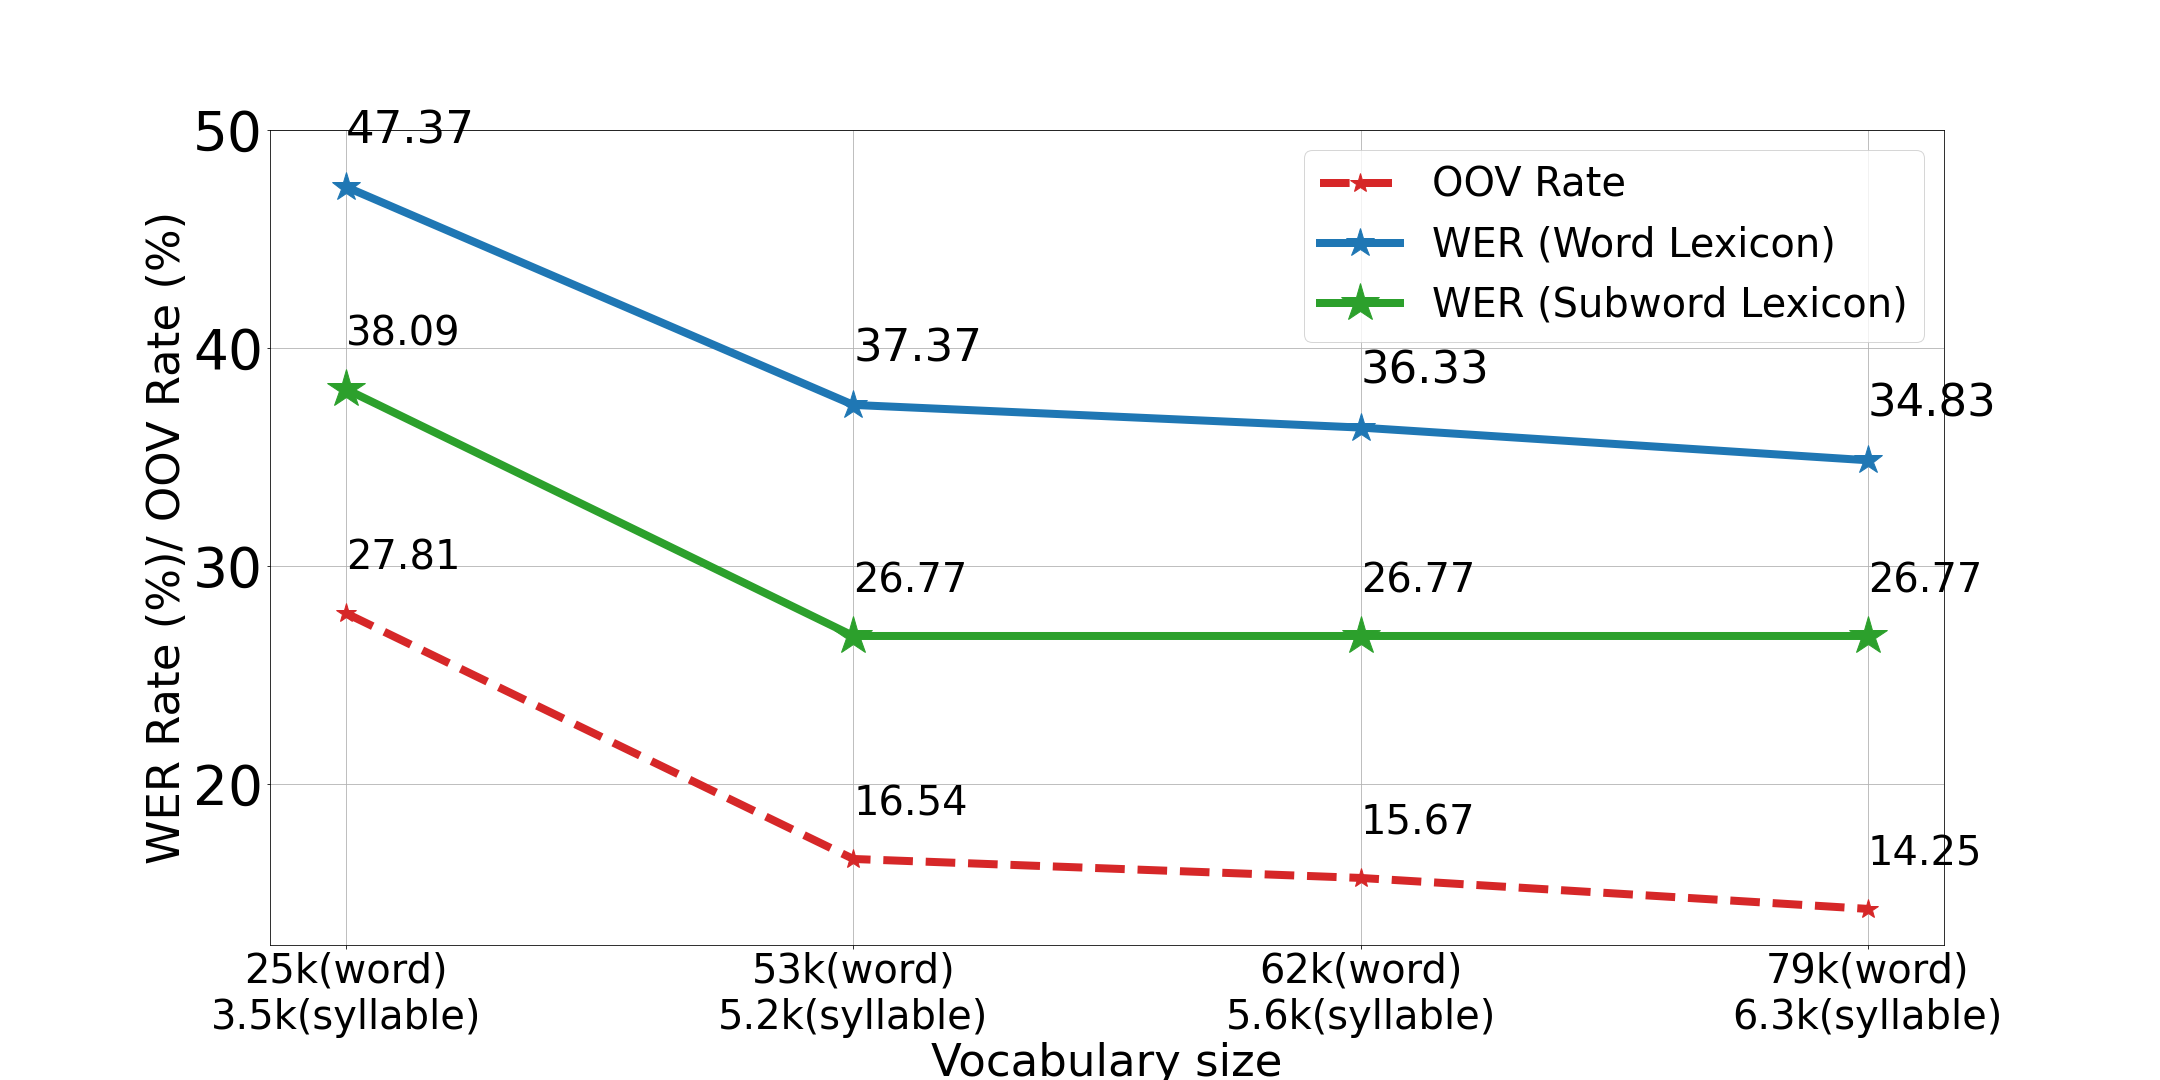
\includegraphics[width=\linewidth]{trigramT2.png}
	\caption{Plot showing WER obtained in Malayalam ASR experiments with word based and syllable subword based language models and lexicons. Word vocabulary sizes are indicated on x-axis.}
			\label{subword}
%
\end{figure}
\subsection{ASSISTED PRONUNCIATION LEARNING}

It is important for a new script learner to understand the pronunciations correctly and get a comprehensive idea  of phonetic features of the text. Mlphon provides phonetic feature tags corresponding to every phoneme. A web interface\footnote {Mlphon Web Interface \url{https://phon.smc.org.in/}} has been developed for user friendly access to  Mlphon features. As demonstrated in Fig. \ref{mlphon-web}, the graphical user interface accepts a word in Malayalam script and  provides syllabification, phonetic analysis and IPA transcription. 

\begin{figure}[h]
	\centering
	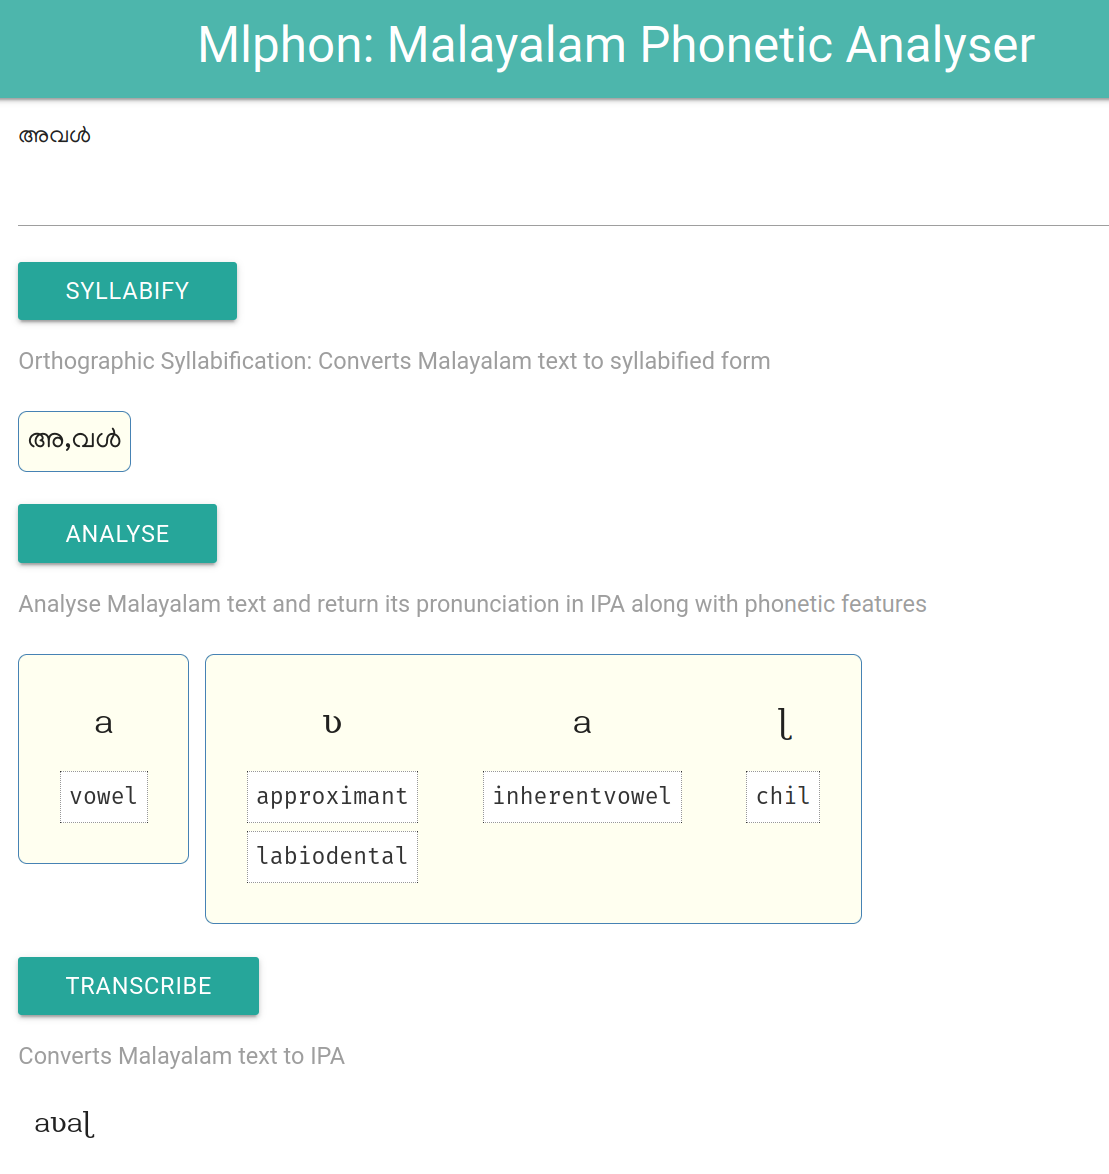
\includegraphics[width=\linewidth]{mlphon-web.png}
	\caption{Web interface for Mlphon. Features of syllabification, phonetic analysis and IPA transcription are shown.}
	% \Description{Phonemic diversity analysis of various speech corpora used in ASR Experiments. The graphs indicate all corpora are equally diverse.}
	\label{mlphon-web}
\end{figure}

This interface can aid even a non native linguistic researcher to analyse and understand the nuances of Malayalam script and pronunciation.





\subsection{Phonemic Diversity Analysis of Speech Corpora}

Speech corpus used in developing ASR and TTS systems has to be phonemically balanced and rich to ensure proper acoustic modeling  \cite{malviya2016structural}. We transcribed the speech corpus transcript to phonemised text using Mlphon. The phoneme diversity of the resulting text is then analysed. The graph in Fig. \ref{phoneticrichness} illustrates the phonemic richness of the corpora used in the ASR experiments described in Section \ref{asr}. The phoneme with the highest number of appearances is the inherent vowel {\ipa /a/}, followed by the vowel {\ipa /i/} in all the corpora under consideration. The most frequent consonant phoneme is the dental plosive {\ipa  /t̪/} in Indic TTS  \cite{baby2016resources} corpus while it is {\ipa /n̪/} in OpenSLR \cite{he-etal-2020-open} and  Festvox IIITH \cite{prahallad2012iiit} corpora. The statistical analysis of phonemes could potentially be used to design corpora with phonemically balanced content \cite{torres2019emilia}.


\begin{figure*}[h]
	\centering
	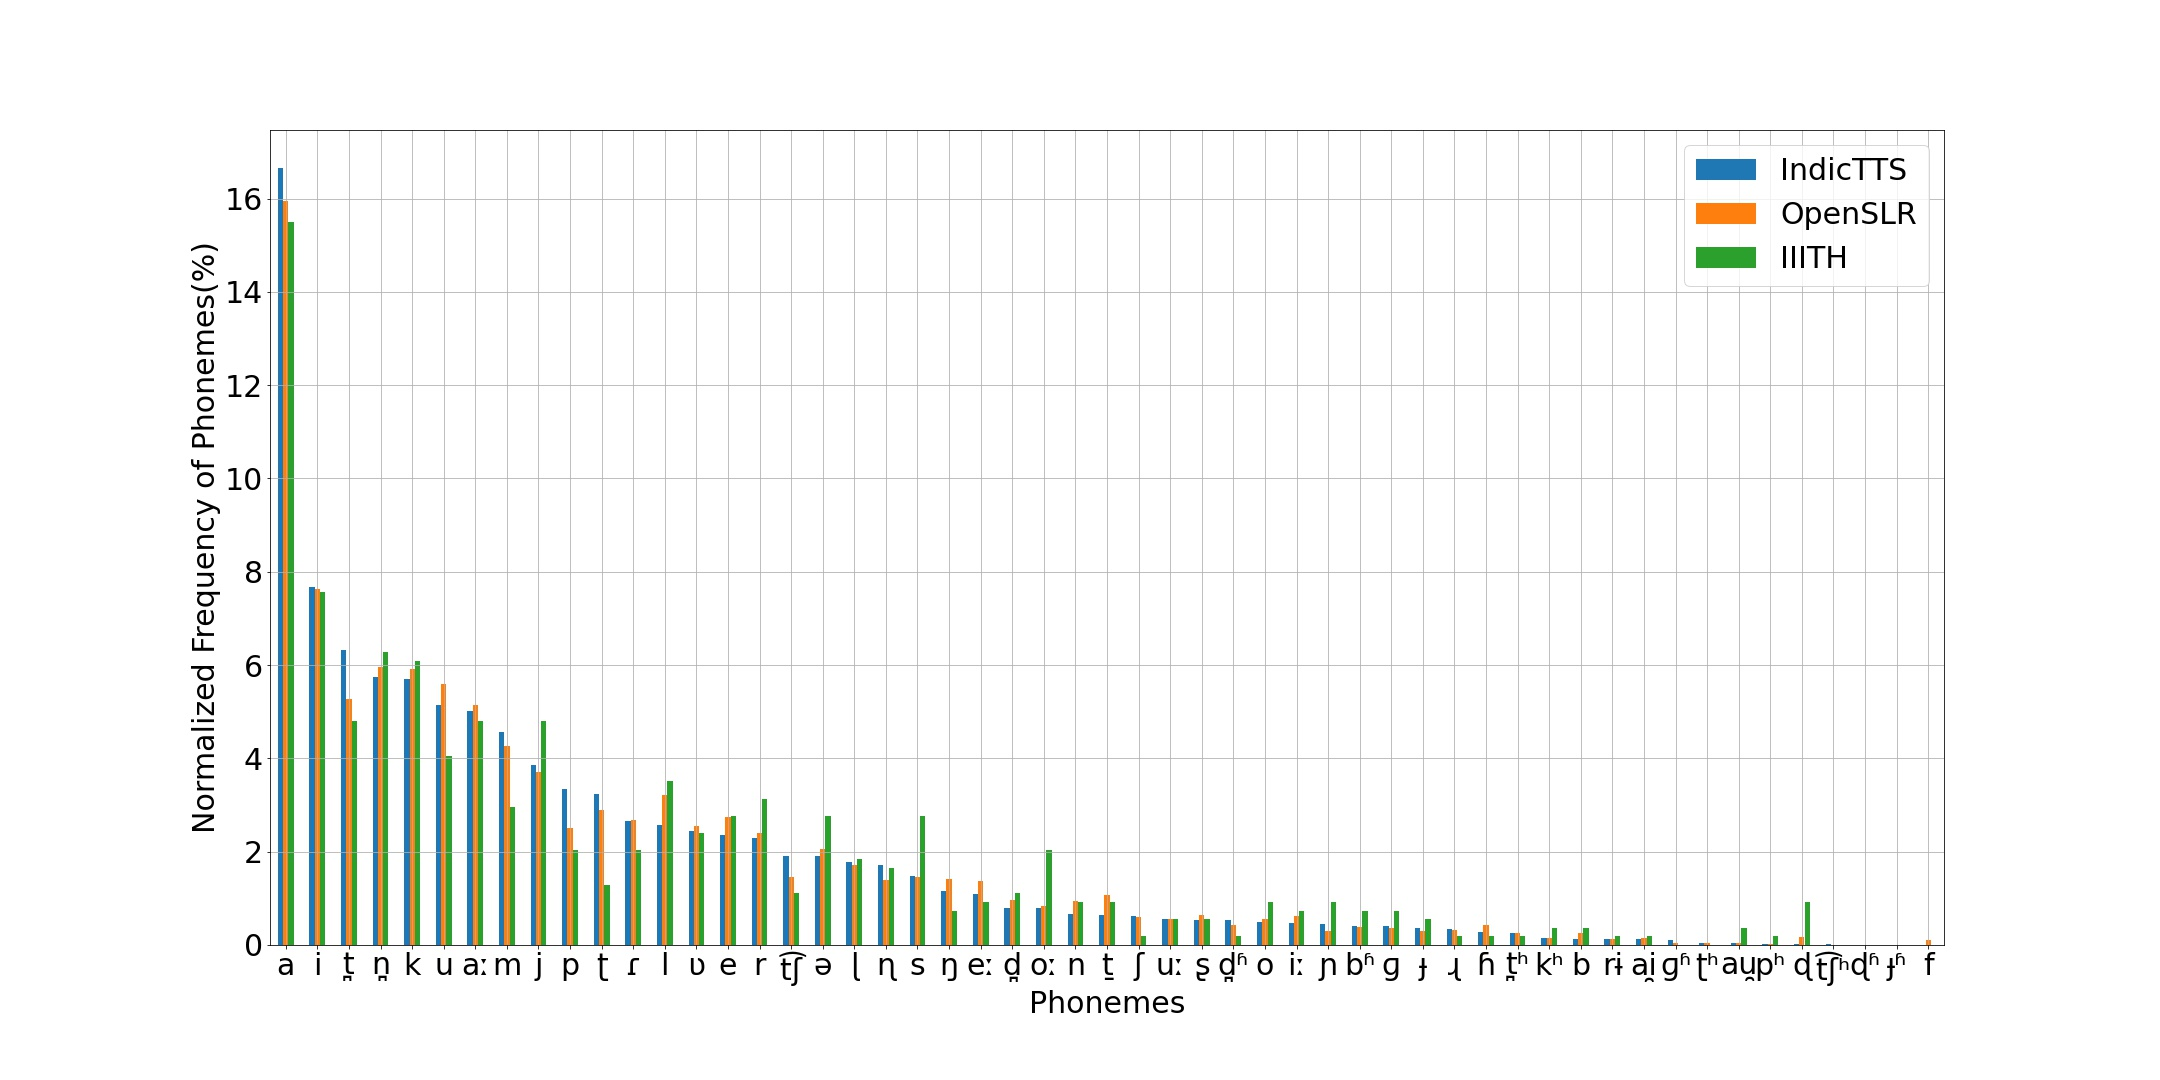
\includegraphics[width=\linewidth, trim=1cm 1cm 2cm 2cm,clip]{phoneticrichness.jpg}
	\caption{Phonemic diversity analysis of various speech corpora used in ASR Experiments. It indicates relative frequency of each phoneme.}
	% \Description{Phonemic diversity analysis of various speech corpora used in ASR Experiments. The graphs indicate all corpora are equally diverse.}
	\label{phoneticrichness}
\end{figure*}


\subsection{Text Sanity Check and Correction}

Large body of text (web crawled, crowd sourced, curated, transcribed or annotated) is the backbone of training and testing modern NLP solutions of  large language models,  part of speech taggers, text to speech and speech to text systems. Mlphon can perform a script grammar check on the text corpora under consideration and give pointers for manually correcting possibly corrupt Malayalam text content due to presence of invisible characters, foreign scripts, wrong script order etc.


The Table \ref{sanitycheck} lists the number of tokens flagged as errors after script grammar check using Mlphon in various Malayalam speech corpora. These flagged errors were corrected before feeding them for training in ASR experiments explained in section \ref{asr}. However, errors which do not violate the script grammar rules can not be detected by Mlphon.

\begin{table}[!h]
\caption{Number of word tokens flagged as invalid by Mlphon on different transcribed speech corpus and corresponding error rates.}
\label{sanitycheck}
\begin{tabular}{lcc}
\hline \hline
Speech Corpora & Error Count & Token Error Rate \\
\hline
Indic TTS \cite{baby2016resources}& 1013 & 1.2\% \\
OpenSLR \cite{he-etal-2020-open}& 83 & 0.3\%\\
Festvox IIITH \cite{prahallad2012iiit}& 22 & 0.3\% \\
Indic Speech \cite{srivastava-etal-2020-indicspeech}& 4337 & 4.3\%\\
\hline
\end{tabular}
\end{table}
\vspace{0.2cm}
% \section{Potential Applications}
% \label{scope}



% \subsection{}



% \subsubsection{Malayalam Poetic Metre Identification}

% Structural classification of Malayalam poetry in terms of poetic metre is based on the properties of orthographic syllable \cite{namboodiri2007using}. The syllabification module could potentially be used for poetic metre identification in Malayalam.

% \subsection{Text Transliterator}

% The grapheme-phoneme converter module in Mlphon can serve as a transliterating unit. It would enable a casual reader who is unfamiliar with the original Malayalam script to pronounce the language reasonably accurately by converting it to IPA, which is universally understood.
 

% For sequence of the syllables $S = s_m . . . s_2s_1$, containing m syllables $s_i$, the probability P(S) is given by a syllable based language model and the following formula:

% \begin{equation}
%     P(S) = P(s_1) \prod_{i = 2}^{m} P(s_i |s_{i-1}s_{i-2}...s_2, s_1)
% \end{equation}

% where $P(s_i |s_{i-1}s_{i-2}...s_2, s_1)$  is the conditional probability that $s_i$ will occur, given the previous syllable sequence $s_{i-1} , . . . , s_1$. With the N-gram approximation, conditional probability is defined by the analogous formula limited to the previous N-syllables only.

% \begin{equation}
%     P(S) = P(s_1) \prod_{i = 2}^{m} P(s_i | s_{i-1}s_{i-2}...s_{i-N+1})
% \end{equation}

% An N-gram language model augments the acoustic model in ASR for reducing the word recognition error rate. We evaluate the syllable based language model on an intrinsic measure called perplexity and on its capability to reduce WER on ASR application.

% Given a language model P(S), where S is the n-syllable sequence, the entropy of the language model can be defined as:


% \begin{equation}
%   H(S) = − log_2 (P(S))
% \end{equation}

% The perplexity PP(S) of the syllable based language model is average number of possible syllables that follow any given syllable sequence in a language. PP(S) is then defined as:

% \begin{equation}
%   PP(S) = 2^{H(W )}
% \end{equation}


% \begin{table}[h]
% 	\begin{center}
% 		\begin{minipage}{250pt}
% 			\caption{Perplexity Measure}
% 			\label{ppl}
% 			\begin{tabular}{@{}cccc@{}}
% 				\hline\hline
% 			 \textbf{N-gram Order} & \textbf{Perplexity}&\textbf{Test Set 1} & \textbf{Test Set 2} \\
% % 		 &                      & OOV: 8\%            & OOV: 1\%\\
% 				\hline
% 				% \multirow{3}{*}{\rotatebox{90}{\textbf{Models} }}
% 				2   &$PP_2(S)$ & 42               & 36               \\
% 			 3  &$PP_3(S)$ &18                & 14             \\
% 			 4 &$PP_4(S)$ &15       &  11       \\

% 				\hline
% 			\end{tabular}
% 		\end{minipage}
% 	\end{center}
% \end{table}


\section{Conclusion}
\label{conclusion}

In this article we presented the requirement analysis, design and the development of a knowledge based computational linguistic tool, Mlphon, using FSTs. The syllabification of graphemes as well as phonemes, phonetic feature analysis and bidirectional grapheme-phoneme conversions that can be performed by Mlphon has applications in speech and linguistic research. The syllabification and grapheme-phoneme conversion capability of Mlphon is evaluated against a gold standard lexicon. Mlphon performs syllabification with an  accuracy of 99\% and syllable error rate of 0.62\% on gold standard lexicon. On grapheme to phoneme conversion task, a phoneme recognition accuracy of of 99\%  with a phoneme error of  0.55\% is observed. The pronunciation lexicons generated with Mlphon has improved performance in terms of WER, than other automated tools when employed in ASR task as described in this article. Mlphon has a high word processing speed when compared to other tools for g2p mapping. The pronunciation lexicon with 100k common words, verbs, nouns and foreign language words in phonemised and syllabified forms published along this work is the first of its kind in Malayalam.  Mlphon that takes care of the script specific contextual rules for phonemic analysis serve as a useful resource for various NLP tasks including ASR, TTS, syllabification for language modeling, phonemic diversity analysis, assisted pronunciation learning and text sanity check as demonstrated in this article.
\appendices


\section{Open Resources published with this work}
\label{resources}
\begin{enumerate}
    \item \href{https://phon.smc.org.in/}{Companion Website for this paper} 
	\item \href{https://github.com/kavyamanohar/mlphon}{Source code of Mlphon}
	\item \href{https://pypi.org/project/mlphon/}{Mlphon Python library}
	\item \href{https://gitlab.com/kavyamanohar/malayalam-phonetic-lexicon}{Malayalam Pronunciation Lexicons}
	\item \href{https://gitlab.com/kavyamanohar/asr-malayalam}{Malayalam ASR experiments using Kaldi}
\end{enumerate}

\bibliography{mlphon-asr}


\begin{IEEEbiography}
[{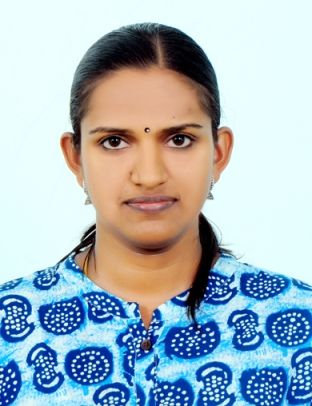
\includegraphics[width=1in,height=1.25in,clip,keepaspectratio]{a1.jpg}}]{Kavya Manohar} received B.Tech. degree from the University of Kerala, India in 2010 and M.Tech. degree from the University of Calicut, Kerala, India in 2012. Since 2013, she has been serving as Assistant Professor in Electronics and Communication Engineering in Engineering Colleges under University of Calicut. She joined College of Engineering Trivandrum, India to pursue her Ph.D. in 2019.  Her research interest includes the Computational Linguistics, Speech Processing and Automatic Speech Recognition.


\end{IEEEbiography}

\begin{IEEEbiography}[{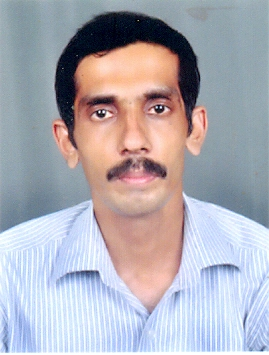
\includegraphics[width=1in,height=1.25in,clip,keepaspectratio]{a2.jpg}}]{A R Jayan}  received his B. Tech degree in Electronics and Communication from Government Engineering College, Thrissur, India in 1992; M. Tech degree  in Electronics from Cochin University of Science and Technology, India in 1994; Ph.D. from  Indian Institute of Technology, Bombay, in 2014. He currently serves as Professor in the Department of Electronics and Communication Engineering, Government Engineering College, Thrissur, India. He holds two patents for his work on consonant-vowel-ratio modification for improving speech perception. His research specialization is in Speech Signal Processing.

\end{IEEEbiography}

\begin{IEEEbiography}[{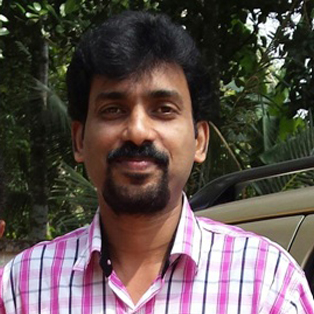
\includegraphics[width=1in,height=1.25in,clip,keepaspectratio]{a3.jpg}}]{Rajeev Rajan} received his B. Tech in Electronics and Communication from College of Engineering,  Adoor (Cochin University of Science and Technology) in 2000; M. Tech in Applied Electronics and Instrumentation  from  College of Engineering, Trivandrum in 2004; Ph.D. from the Dept.  of Computer Science and Engineering, Indian Institute of Technology, Madras, Chennai in 2017. He currently serves as Associate Professor in the Department of Electronics and Communication Engineering, College of Engineering Trivandrum, India.  His research areas are Speech and  Music Signal Processing.


\end{IEEEbiography}

\EOD

\end{document}



